\chapter{Simulation Outcomes}\label{chap:simulationoutcomes}
In the following the load balancing algorithms are abbreviated. The Single-Proposal Deal-Agreement-Based algorithm is abbreviated as DAB, the Push-Pull Sum algorithm is abbreviated as PPS and the Adaptive Threshold Push-Pull-Sum algorithm is abbreviated as ATPPS. The simulation outcomes are presented in plots, mostly log-log or log-linear graphs (logs for the mean squared error are base 10), since the mean squared error values vary a lot over the 100 rounds of simulation. Figures \ref{fig:completegrapslopes}, <slopes images referencing>  depict the slopes for three distinct regions (of the x-axis) and the general slope over all the 100 rounds. For each algorithm the function that distributes the mean squared error over the rounds is model fitted with the models of linear regression, polynomial regression, exponential decay or logarithmic regression, depending on the best-fit.

\textbf{Linear Regression}: The linear regression fits $MSE_r=m*r+b$ to the data. Where $m$ is the slope: $\frac{\Delta MSE}{\Delta r}$. In the case of load balancing the slope is mostly negative, meaning that for each round, the $MSE_r$ decreases in comparison to the $MSE_r-1$, the mean squared error of the previous round. $b$ is the mean squared error, in round 0, so in that round where the network is initialized in our experiments. In round 0 the mean squared error is calculated with the unbalanced network, so $MSE_0$ is the initial mean squared error, where no load balancing is applied yet. The 

\textbf{Polynomial Regression}: The polynomial model $MSE_r=a_0+a_1*r+a_2*r^{2}+a_3*r^{3}+...+a_n*r^{n}$ is a model where the mean squared error reduction per round follows a power law relationship. It captures non-linear relationships between the independent variable $r$ and dependent variable $MSE_r$ \cite{MotulskyDataFitting}. Polynomial regression can model non-linear trends like diminishing returns (e.g., rapid MSE reduction initially, then slower reduction). It fits the curvature of MSE decay, even if it's not strictly exponential or linear. Higher-degree polynomials can capture intricate patterns in the reduction of MSE over rounds.

\textbf{Exponential Regression}: The exponential regression model fits $MSE_r=a*e^{-br}$ to the data. Exponential models capture the initially steep drop in mean squared error at early rounds, followed by slower reductions in later rounds. The exponential decay model is also an non-linear model. The initial value of the mean squared error is captured by $a$. In the initializing round where $r=0$, $MSE_r=a*e^{b*0}$ evaluates to $MSE_r=a$. Larger $a$ values indicate larger initial error in the network. The decay rate is captured by $b$. The $b$ value determines how quickly the MSE decreases per round $r$. For the exponential decay model $b$ is negative. A larger negative value for $b$ indicates a faster error reduction in the network, while values closer to 0 indicate slower error reduction.

\textbf{Logarithmic Regression}: The logarithmic regression models data as $MSE_r=a+b*\log{(r)}$. $a$ is the initial mean squared error, when $\log{(r)}=0$. $b$ is the rate of reduction per unit of logarithmic increase in rounds. A large positive $b$ decreases the error faster.

\todo{The polynomials before chapter ROC are in the wrong order constant term is the last term and so on. Correct that and the analysis of that.}

\section{Complete Graph}\label{sec:completeGraph}
Figures \ref{fig:completegraphMSEperRoundLogLog} show the mean squared error reduction over the rounds for the three load balancing algorithms simulated on the complete graph on a log-log graph.

%\begin{figure}[h]
%    \centering
%    \scalebox{0.5}{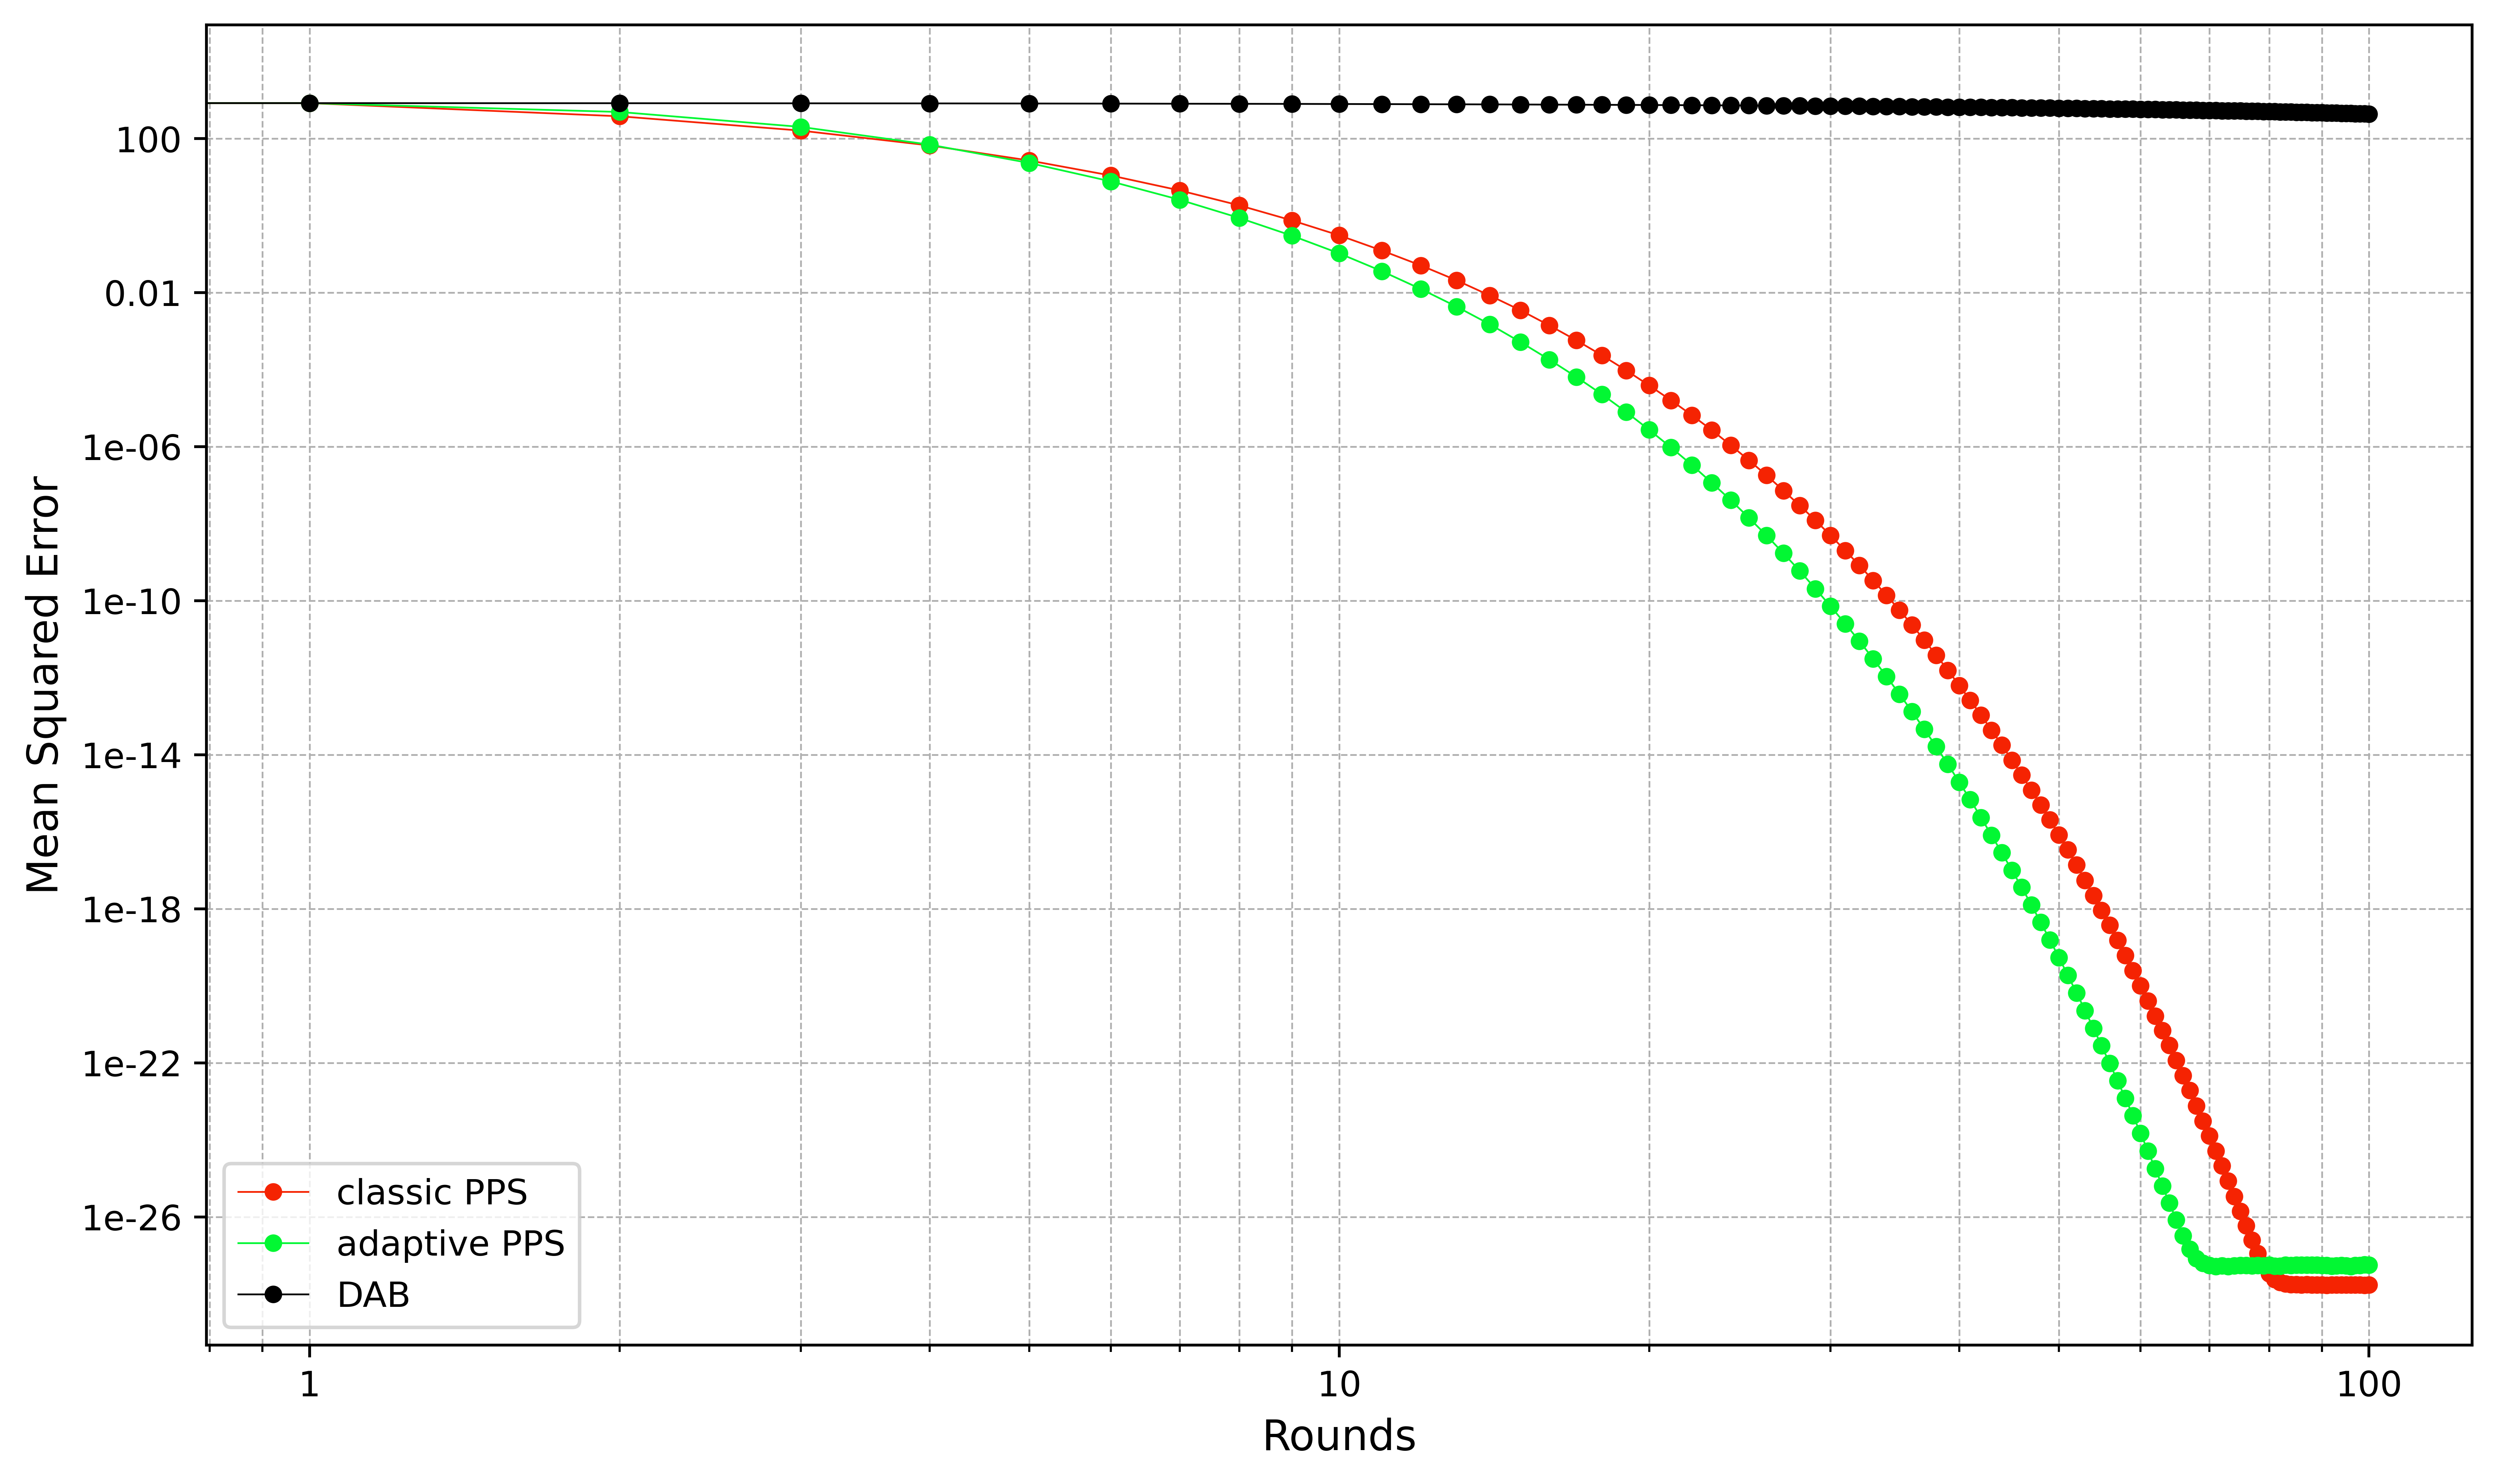
\includegraphics{figures/Simulation_outcomes/CompleteGraph/DAB_vs_PPS_CG_r100_n1024_averaged_loglog.png}}
%    \caption{Complete Graph: mean squared error per rounds (log-log)}
%    \label{fig:completegraphMSEperRoundLogLog}
%\end{figure}

\textbf{Deterministic Agreement-Based Algorithm (DAB)}: One can observe that the black line shows constant mean squared error reduction, indicating that this algorithm does not improve the load balance by much over time. The DAB performs poorly due to the rigid determinism; DAB uses a fixed, deterministic load redistribution rule, where one node looks for the minimal loaded neighbor and proposes to that node. Since for the complete graph each node are interconnected, the neighbors with the minimal loads are the same for every node. Thus, the deterministic strategy proposing to the minimal neighbor does not distribute load in suboptimal ways. The number of load transfers in this scenario per round is very limited, resulting in poor mean squared error reduction. The main observation is that deterministic methods can struggle in high-connectivity environments because they fail to exploit randomness or adaptivity. Figure \ref{fig:dabCompleteModelFit} shows the exponential regression fit for the MSE data when the DAB algorithm as a load balancing algorithm is applied to the network. The fitted curve is expressed by the equation $MSE=844.63*e^{-0.01}*r$. The decay rate of -0.01 suggests a very slow decrease in MSE. The fitted curve and model seem very suitable for the MSE data, since the fitted curve aligns with the MSE data. In summary, the exponential regression model captures the slow and steady MSE reduction of DAB over rounds, highlighting its slow but consistent convergence behavior.

%\begin{figure}[H]
%    \centering
%    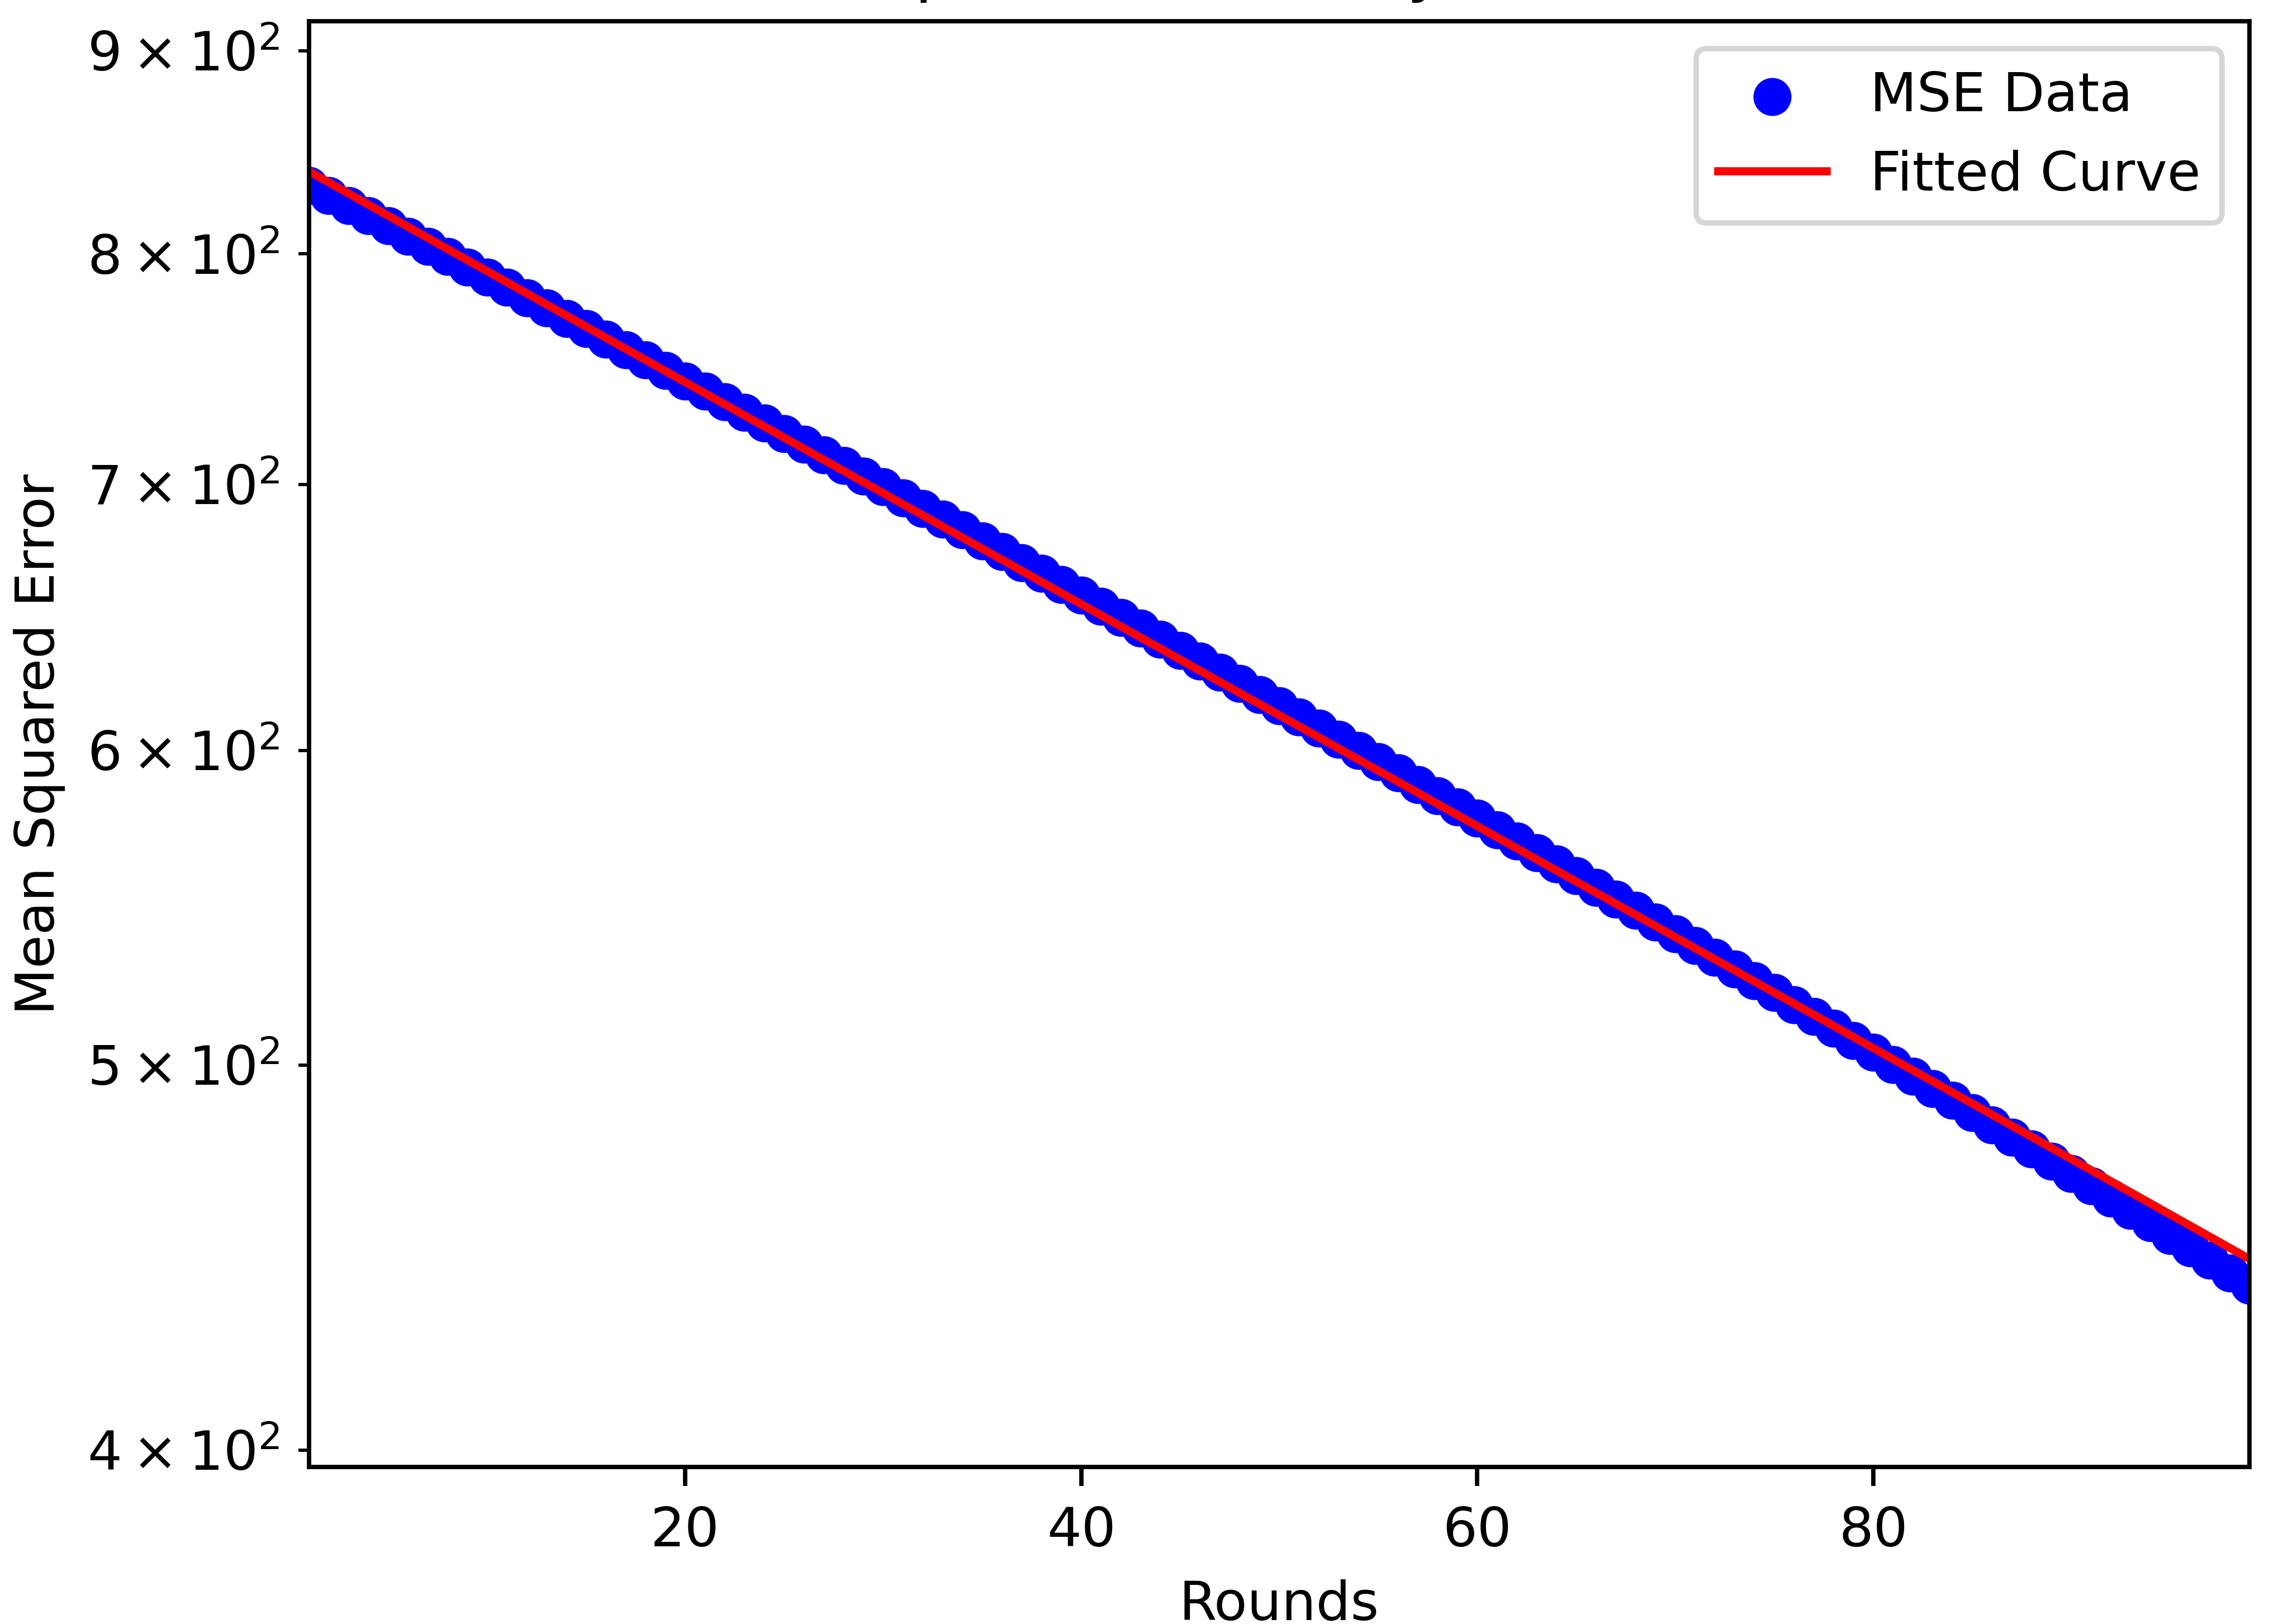
\includegraphics[width=\linewidth]{figures/Simulation_outcomes/CompleteGraph/DAB/DAB_modelfitting_rounds_99_model_1.png}
%    \caption{Exponential Decay Fit: DAB}
%    \label{fig:dabCompleteModelFit}
%\end{figure}

\textbf{Push-Pull Sum algorithm (PPS)}: The PPS-curve decreases gradually in mean squared error, showing significant error reduction over time. Since all nodes are equally connected, no structural constraints slow down the process of pushing and pulling load from neighbors. Over time, repeated randomized exchanges smooth out load imbalances, leading to a exponential decay in mean squared error. Classic PPS does not differentiate between "highly imbalanced" and "near-balanced" nodes. Load transfers happen uniformly, even when the system is close to equilibrium, which slows convergence in later rounds. Figure \ref{fig:ppsCompleteModelFit} visualizes the MSE data of the PPS load balancing algorithm, plotted for the rounds 10 to 80 and fitted with the exponential regression model. The best-fit follows the equation $MSE=2530.41*e^{-0.9*r}$. The graph uses a logarithmic scale for the mean squared error. The fitted curve aligns closely with the MSE data, so the exponential model accurately describes the behaviour of the algorithm for this region. The decay rate of -0.9 indicates a steep decrease in MSE. This suggests that the PPS load balancing algorithm reduces the MSE in a exponential way.

%\begin{figure}[H]
%    \centering
%    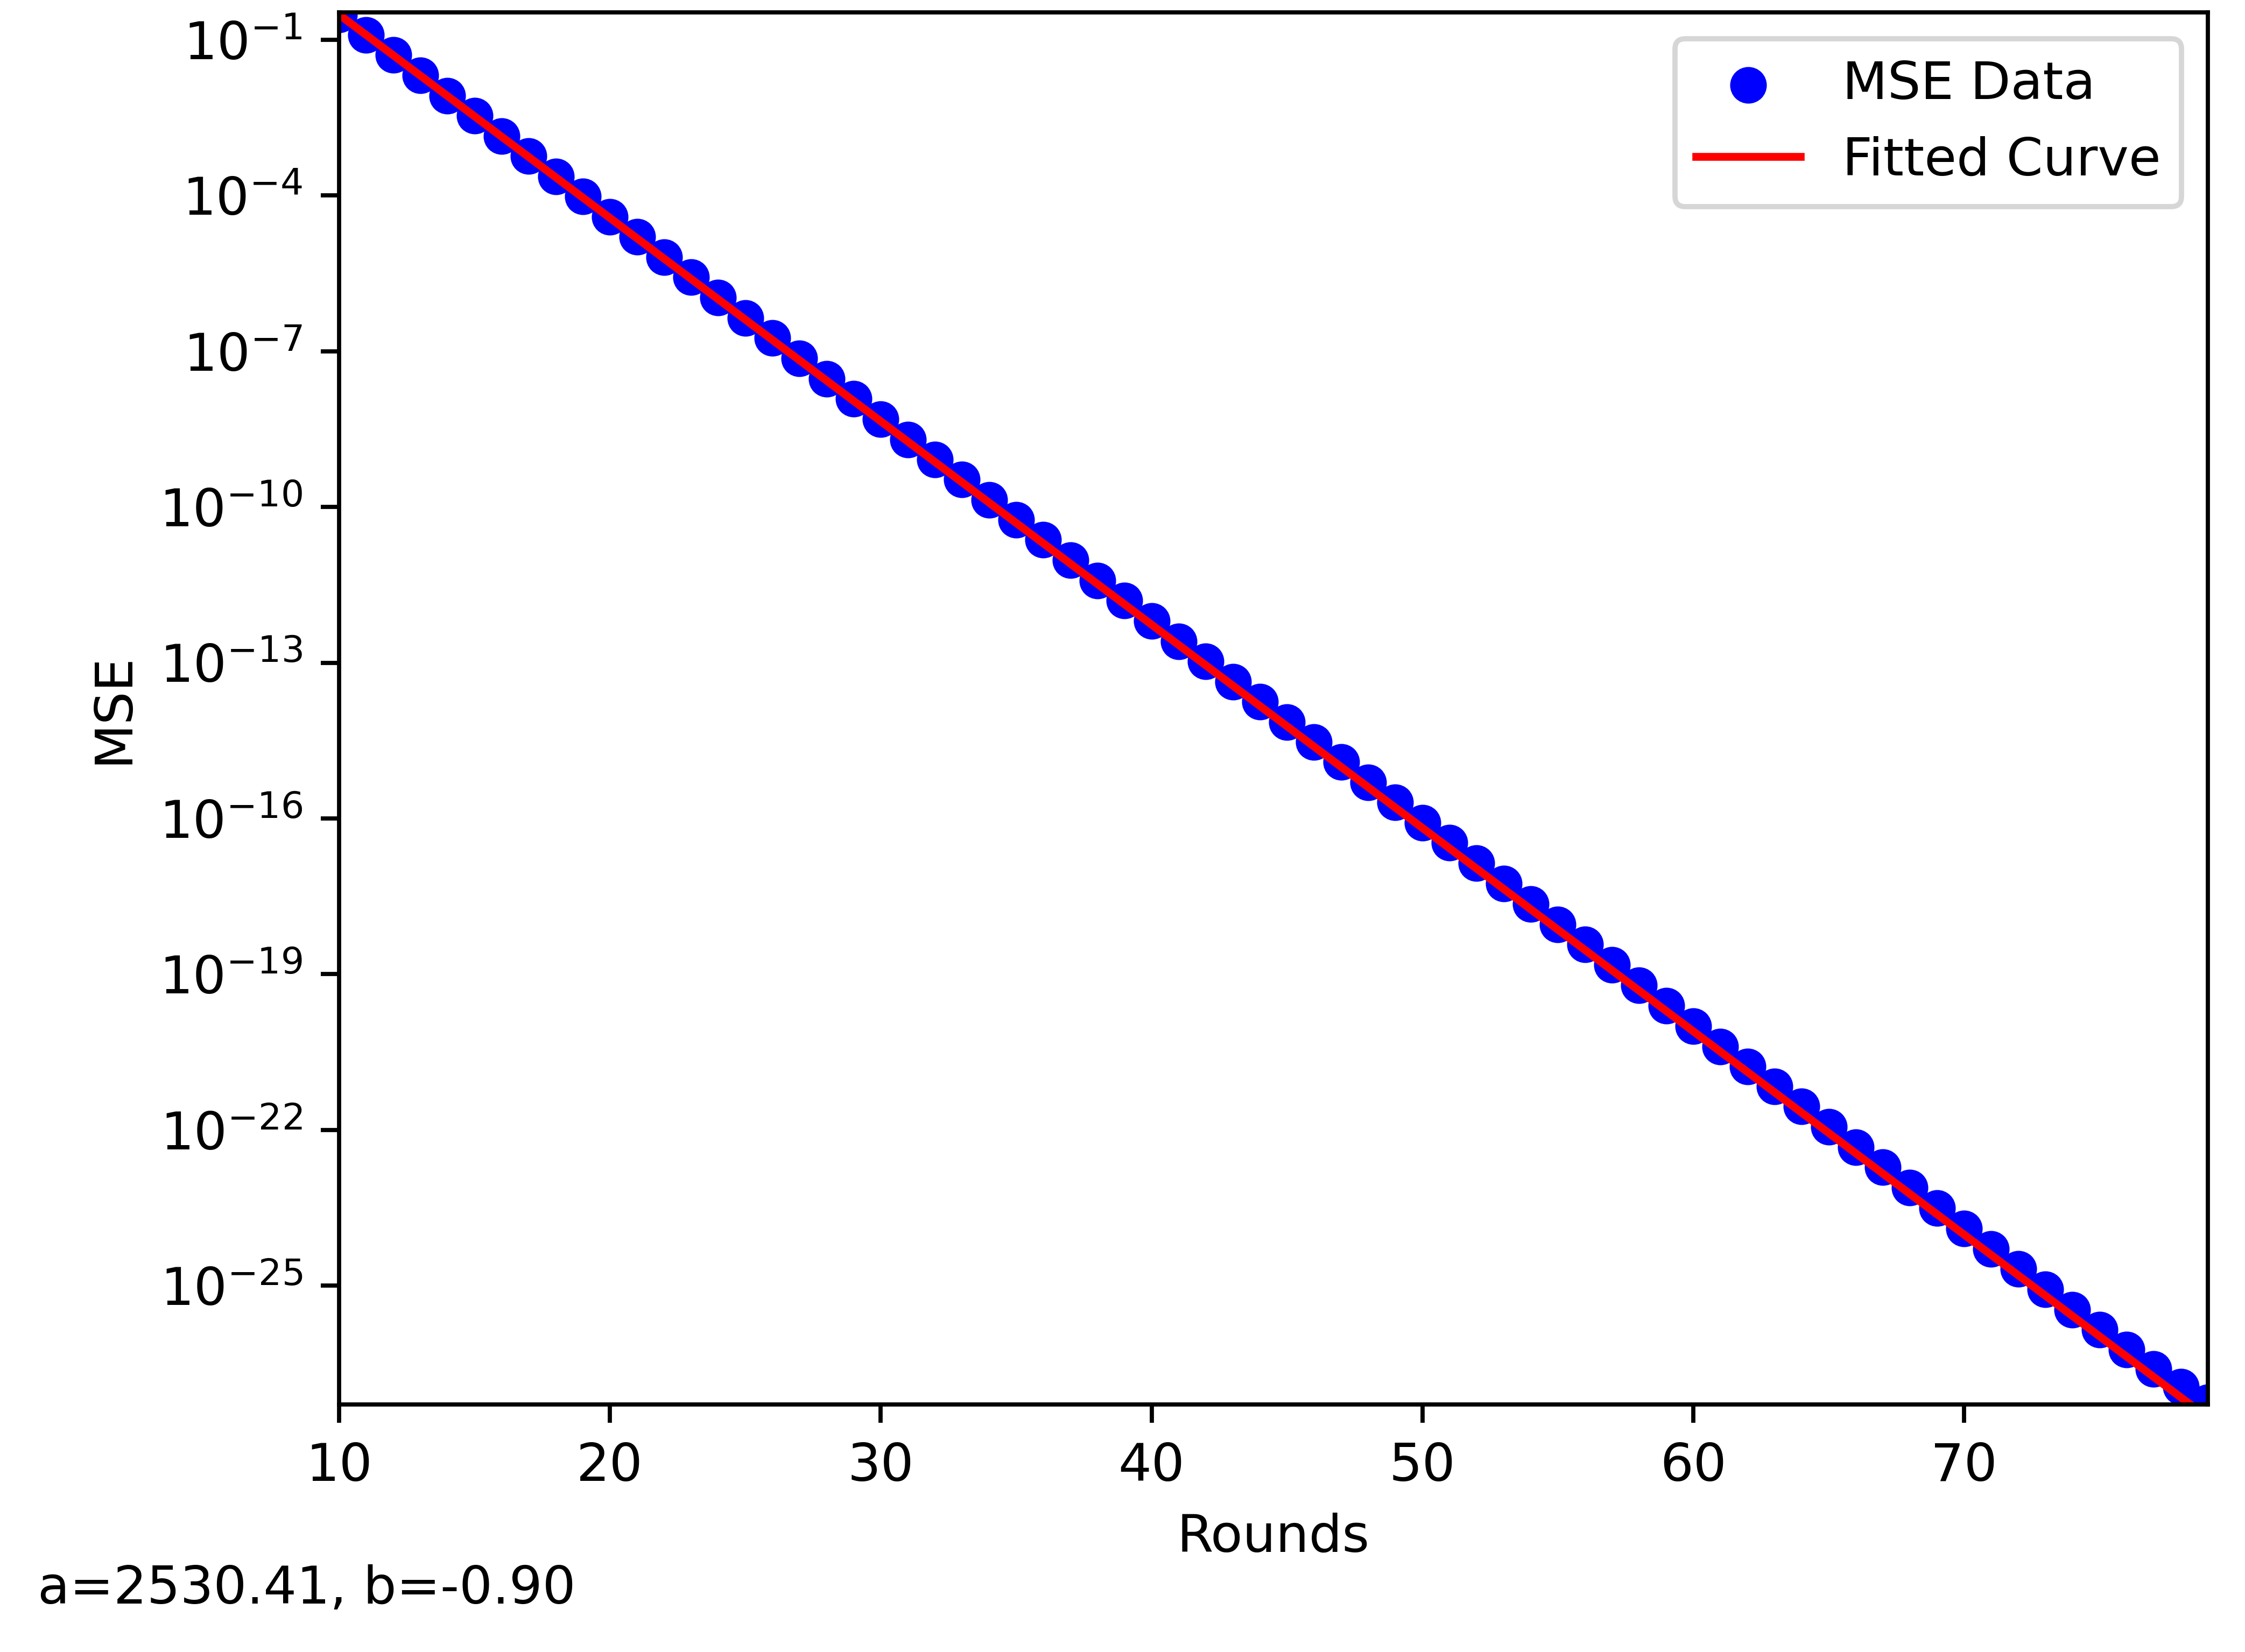
\includegraphics[width=\linewidth]{figures/Simulation_outcomes/CompleteGraph/PPS/PPS_modelfitting_rounds_79_model_1.png}
%    \caption{Exponential Decay Fit: PPS}
%    \label{fig:ppsCompleteModelFit}
%\end{figure}

\textbf{Adaptive Push-Pull Algorithm (ATPPS)}: The ATPPS-curve decreases faster than the red curve, reaching lower MSE values earlier. Adaptive Thresholding: Nodes adaptively decide when and how much load to exchange based on thresholds. For example: Nodes with significantly higher load push more load to neighbors. Nodes closer to balance reduce their interactions. Adaptive strategies reduce redundant exchanges when the system is near equilibrium, focusing resources on nodes with the largest imbalance. In a complete graph, adaptive decisions propagate quickly because every node can directly communicate with others. The adaptive mechanism leverages the symmetry and high connectivity of the complete graph to reduce MSE more quickly and efficiently. In Figure \ref{fig:atppsCompleteModelFit} the exponential regression fit is visualized for the MSE data of the ATPPS load balancing algorithm graph in the complete graph for the rounds 10 to 65. The fitted curve is expressed by the equation $MSE=4309.94*e^{-1.06}*r$. A steep error reduction is indicated by the decay rate of -1.06. As the PPS algorithm the ATPPS algorithm reduces the error very effectively in an exponential manner. Rounds 66 to 100 show a plateauing of the MSE data.

%\begin{figure}[H]
%    \centering
%    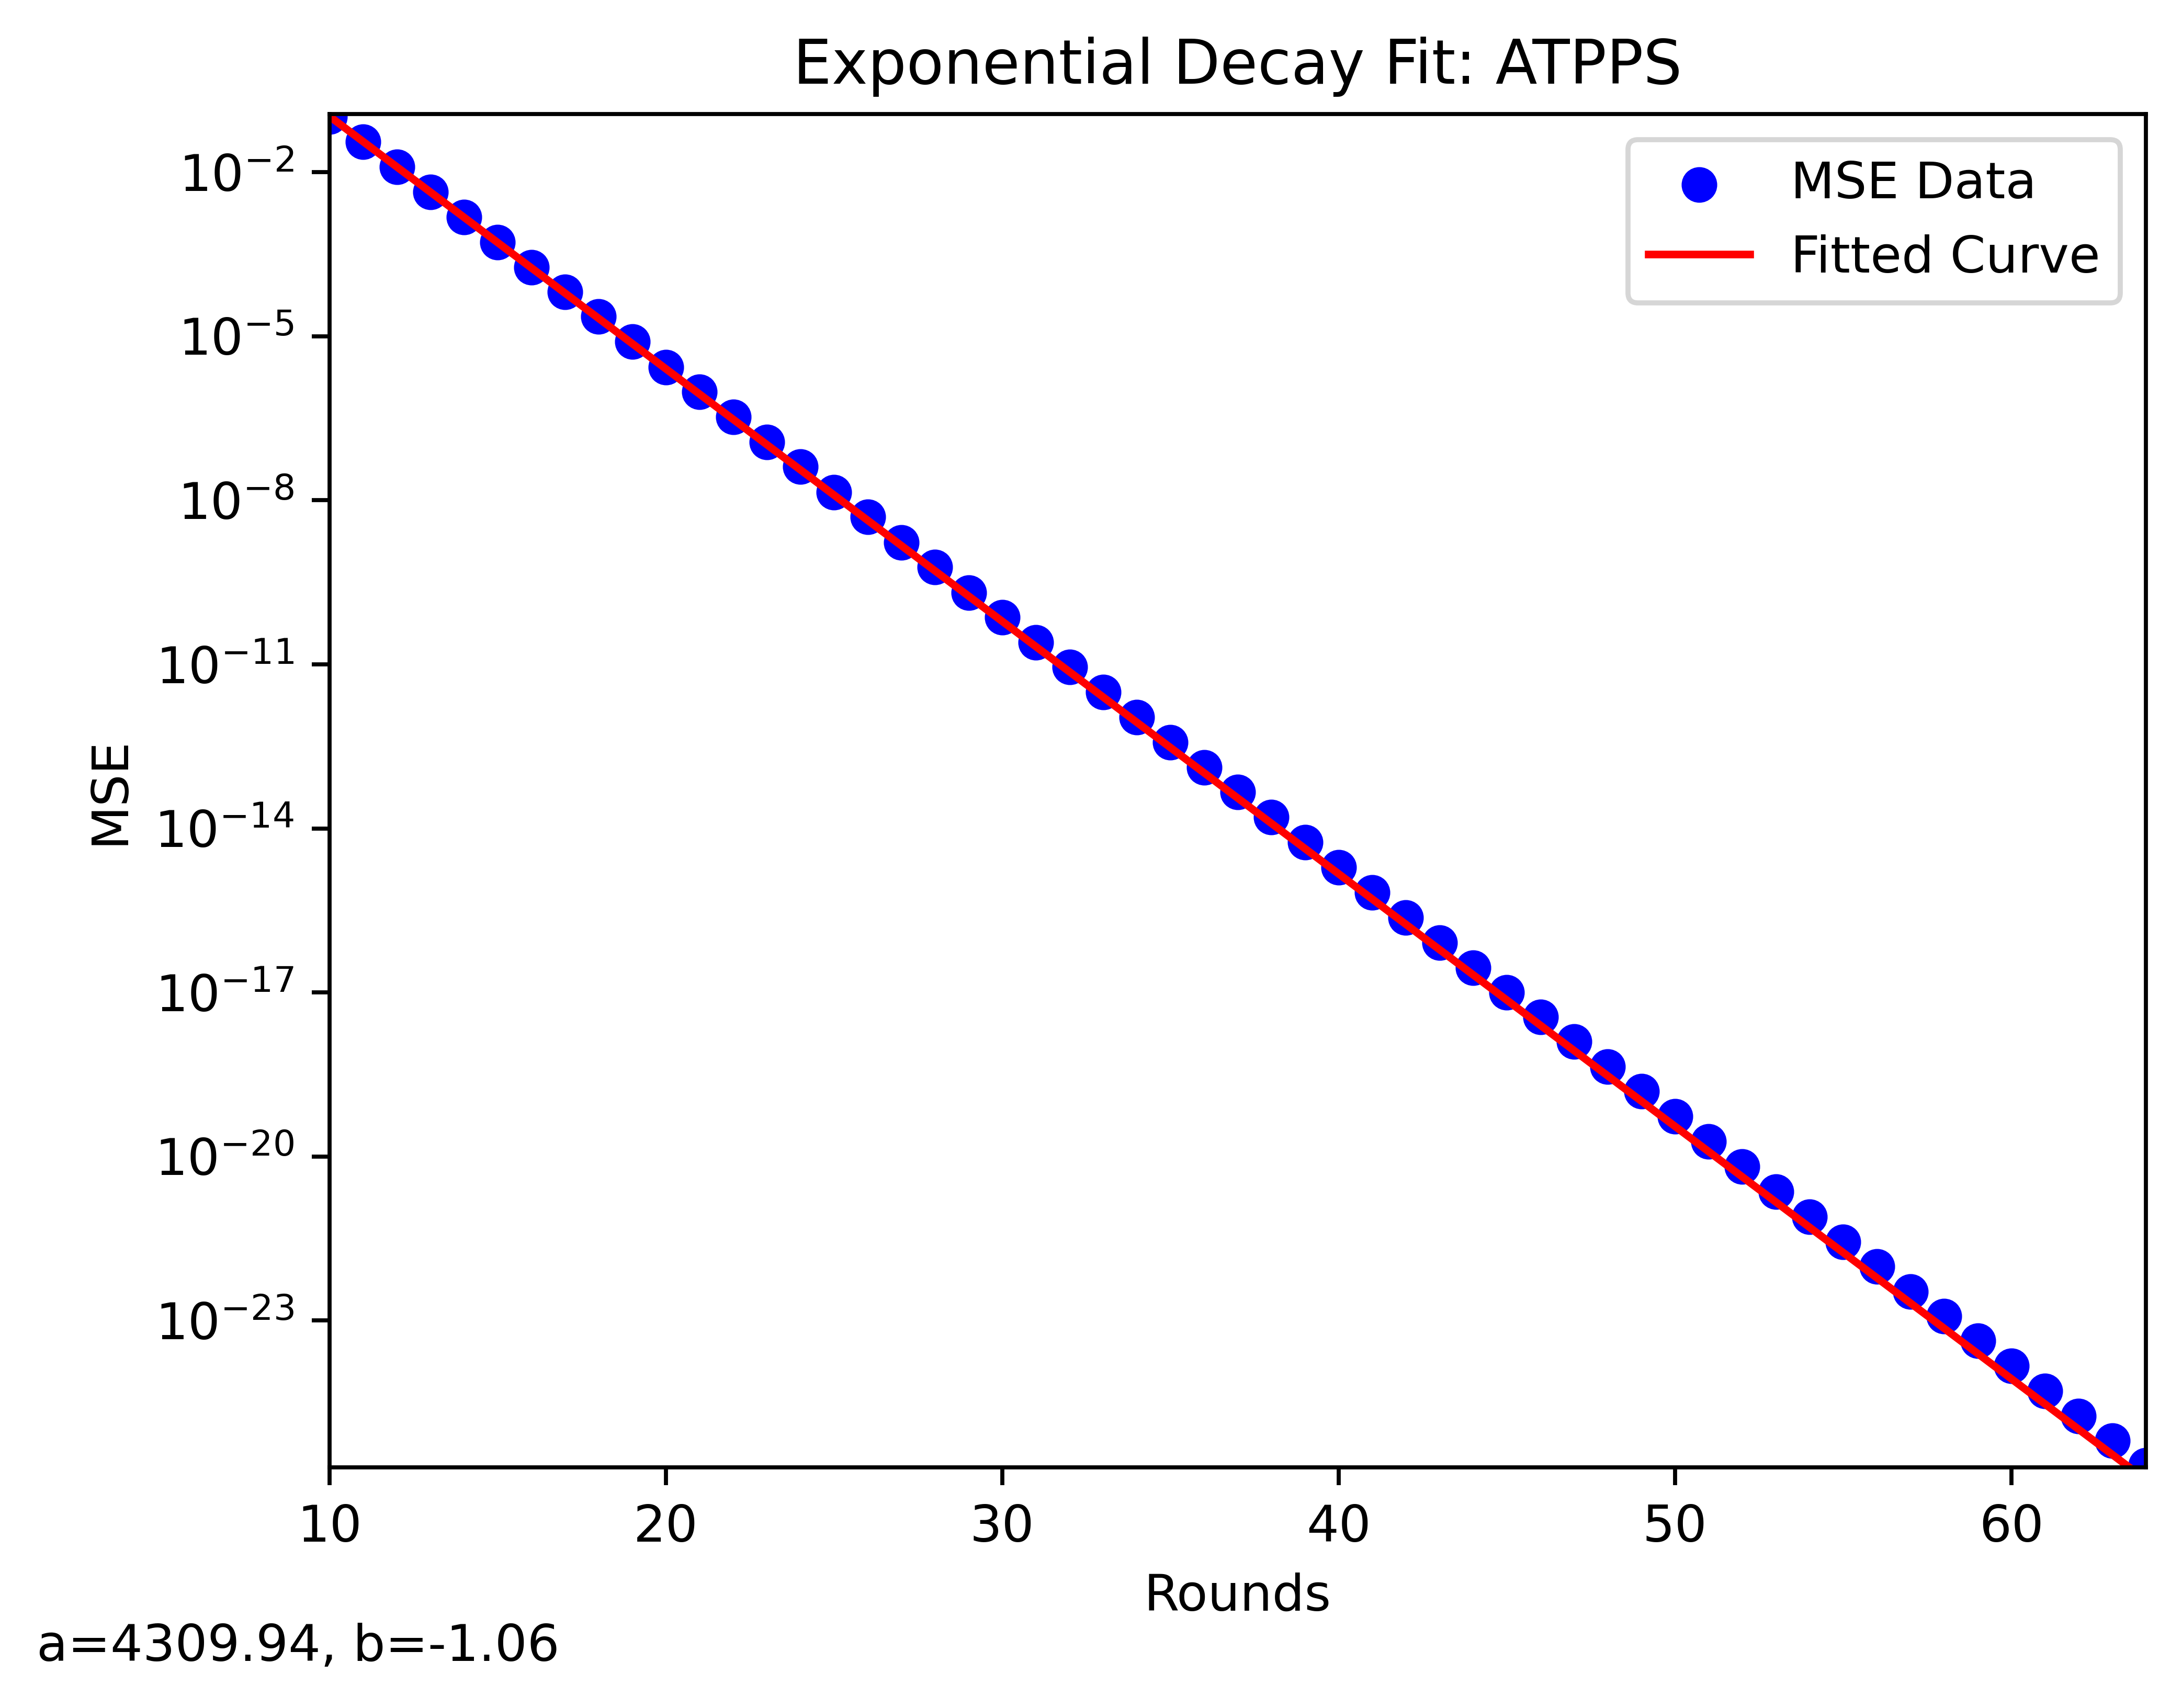
\includegraphics[width=\linewidth]{figures/Simulation_outcomes/CompleteGraph/ATPPS/ATPPS_modelfitting_rounds_64_model_1.png}
%    \caption{Exponential Decay Fit: ATPPS}
%    \label{fig:atppsCompleteModelFit}
%\end{figure}

Figure \ref{fig:completegrapslopes} visualizes a heat map of the slopes (rates of change) for the three load balancing algorithms across different regions of the graph. The values reflect how steeply the mean squared error decreases over rounds. PPS and ATPPS have steep negative slopes in the start region, namely the rounds 1-10 with a value of -92, indicating rapid initial improvement. However, their slopes in the middle (rounds 11-65) and end regions (rounds 66-100) approach zero, suggesting a plateau in performance. DAB has shallower negative slopes overall, reflecting a more gradual and consistent error reduction across all regions. The general slopes (rounds 1-100) for PPS and ATPPS (-8.4) are much steeper than DAB (-4.4), suggesting that PPS and ATPPS converge faster on average. The end region is chosen as 66-100 to catch the trend of plateauing for the ATPPS and also for PPS which is beginning to plateau in errror reduction in later rounds (round $\sim$80-100).

%\begin{figure}
%    \centering
%    \scalebox{0.8}{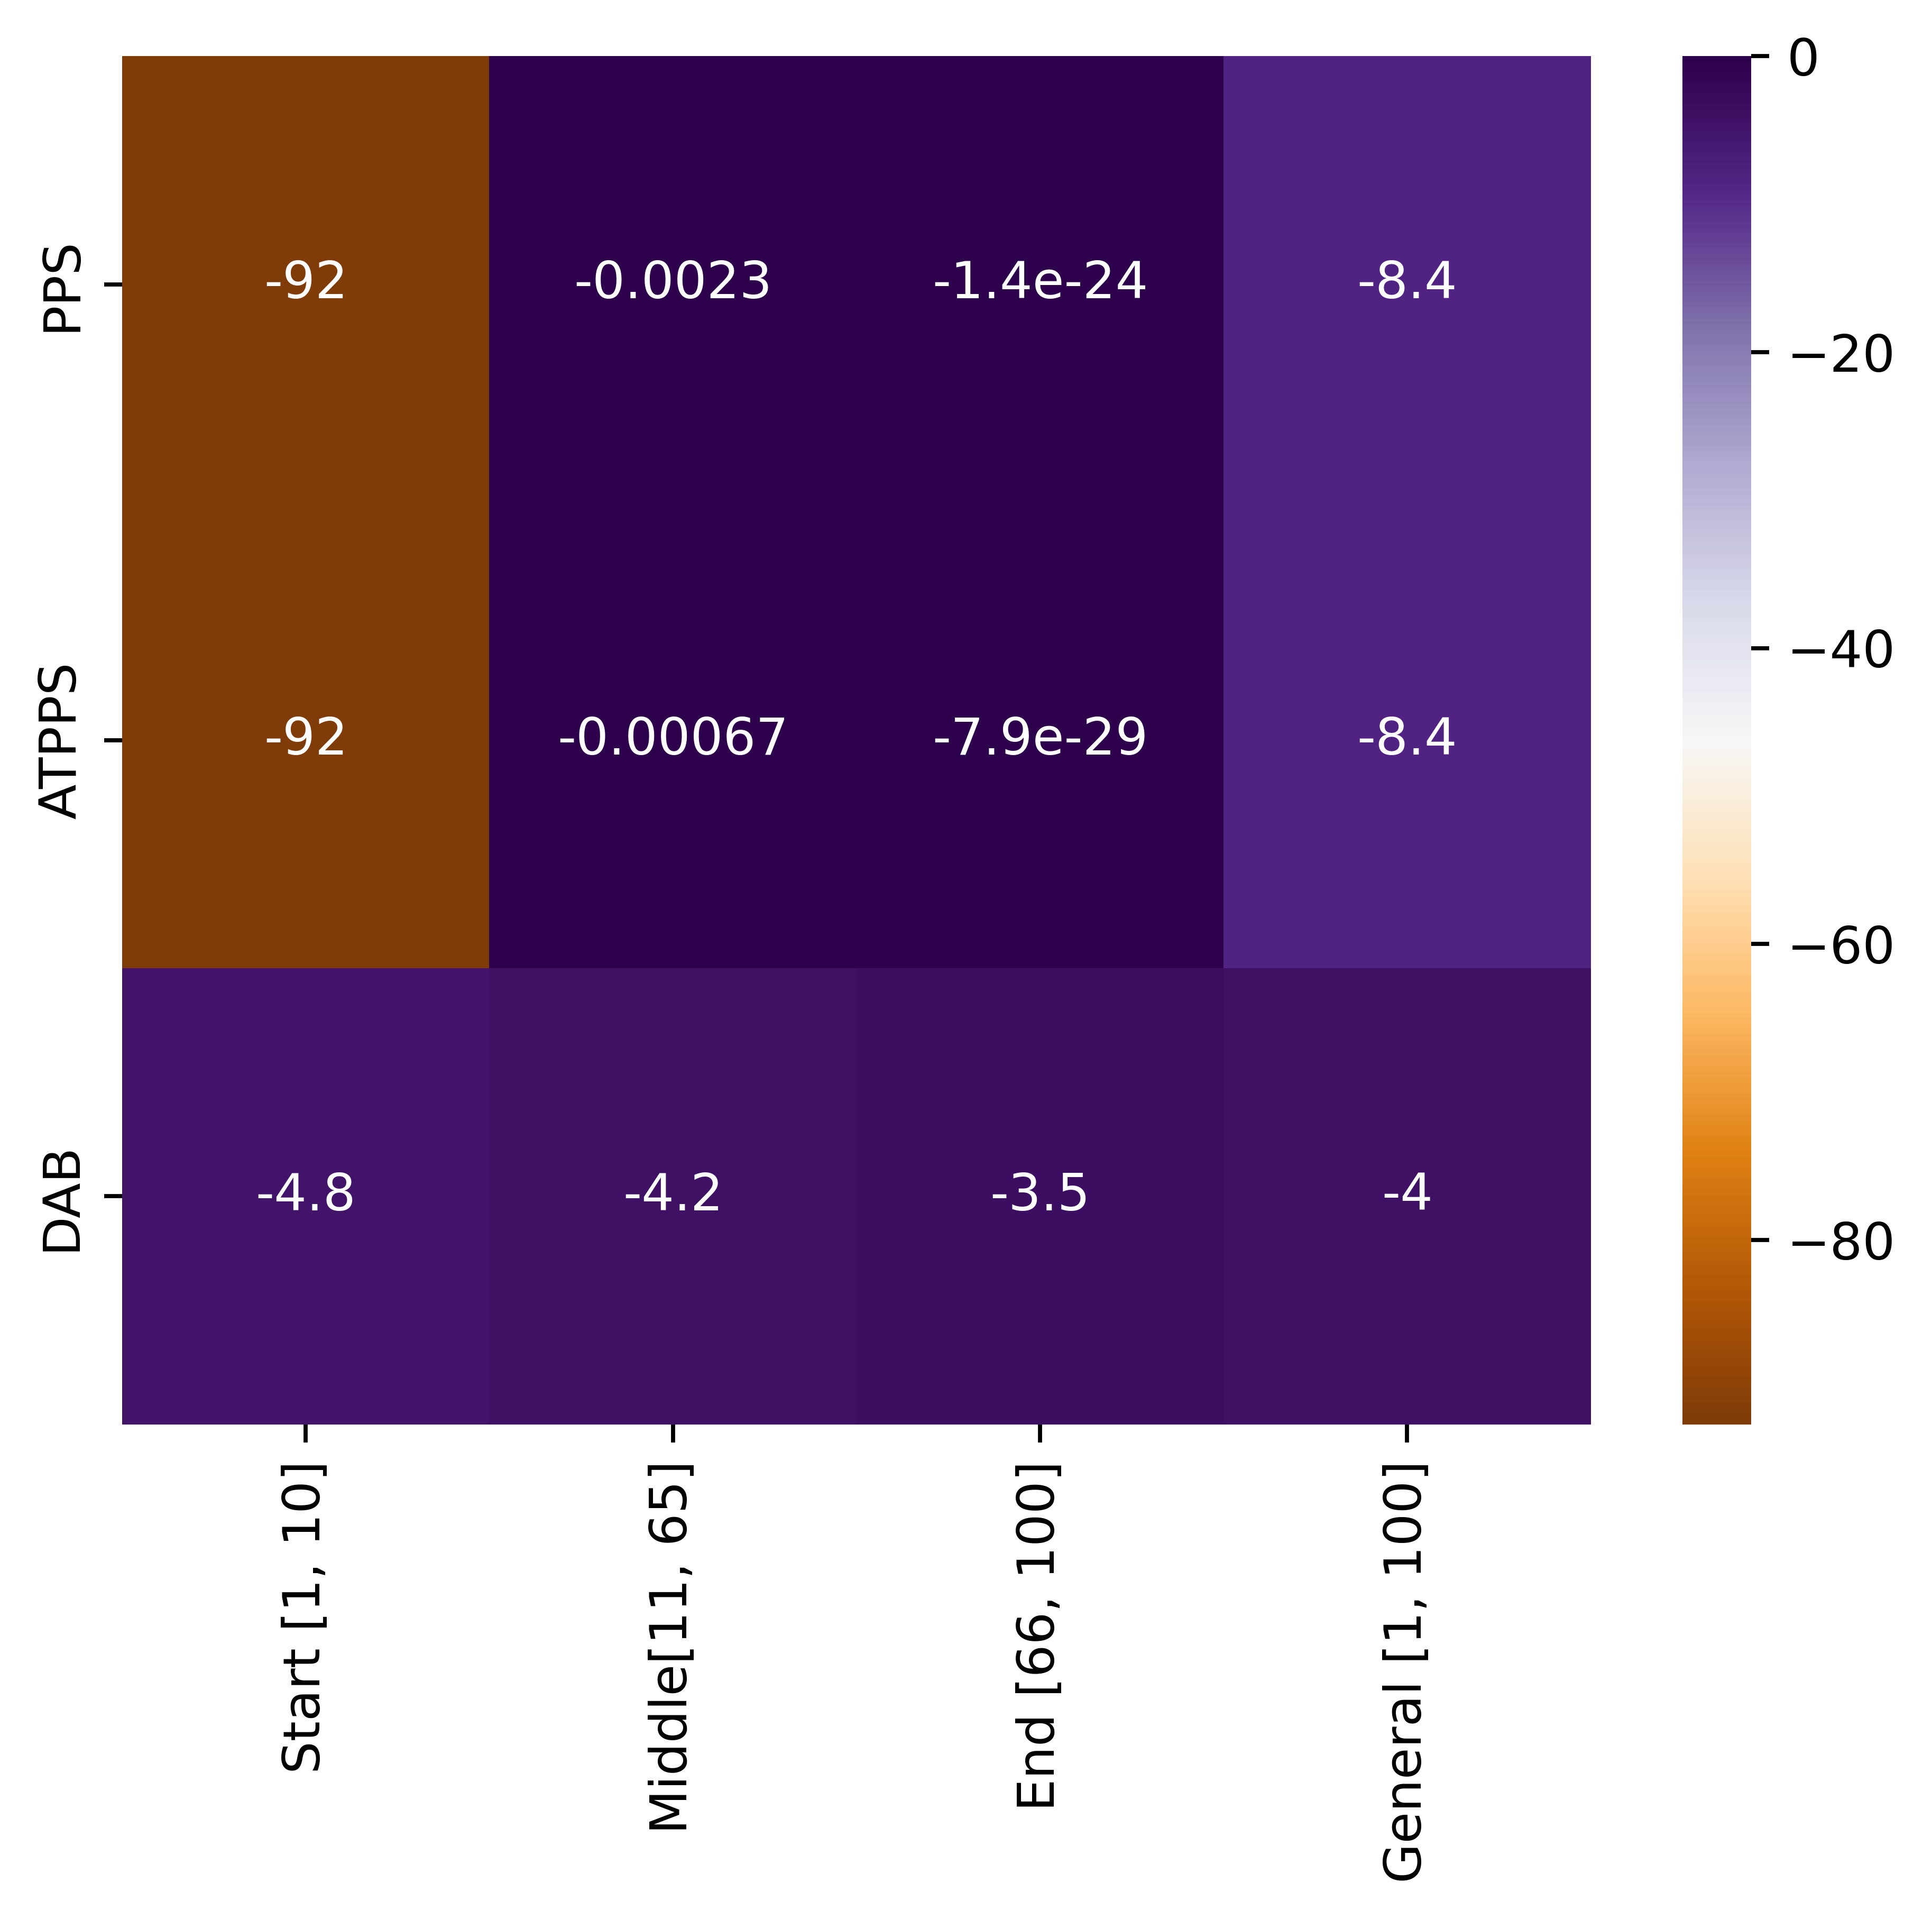
\includegraphics{figures/Simulation_outcomes/CompleteGraph/DAB_vs_PPS_vs_ATPPS_slopesheatmap_100rounds.png}}
%    \caption{Complete Graph: heat map of slopes per region}
%    \label{fig:completegrapslopes}
%\end{figure}


\section{Star Graph}\label{sec:stargraph}
For the star graph the push-pull mechanism-based protocols seem to perform well in MSE reduction, while the DAB algorithm seem to struggle with in this topology as depicted in figure \ref{fig:stargraphMSEperRoundLogLog}

% \begin{figure}[h]
%     \centering
%     \scalebox{0.5}{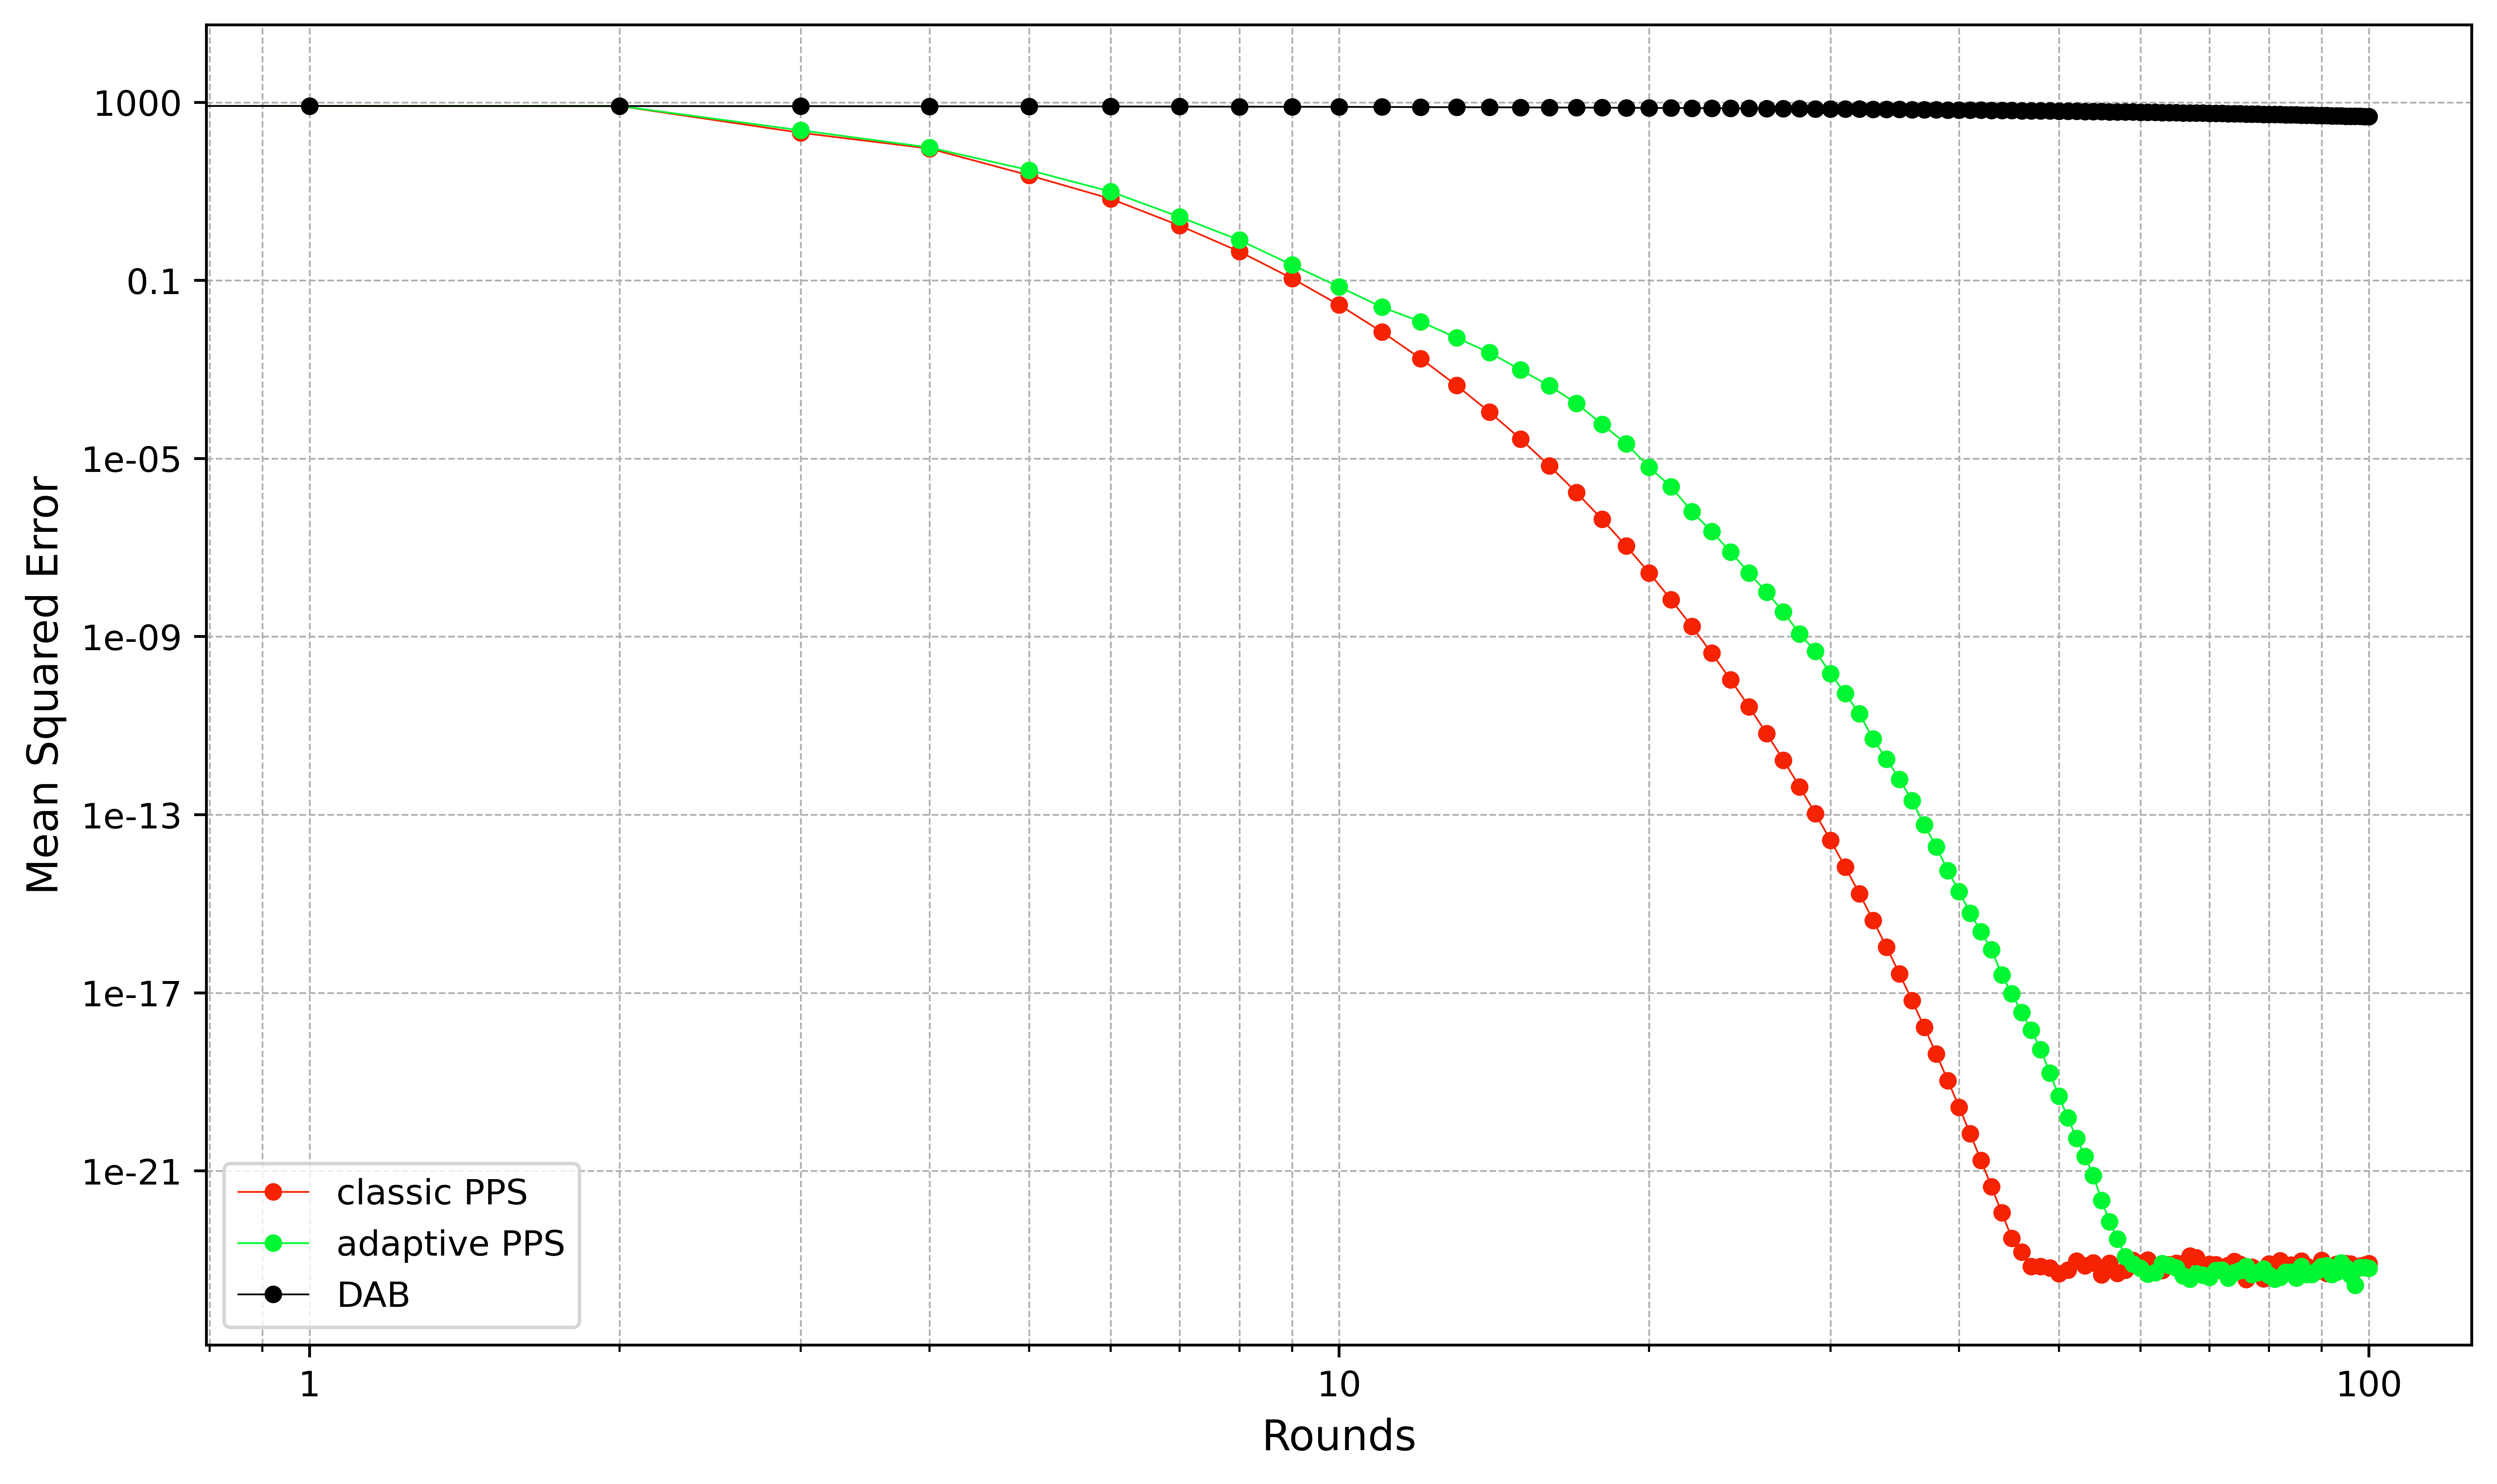
\includegraphics{figures/Simulation_outcomes/StarGraph/DAB_vs_PPS_SG_r100_n1024_averaged_loglog.png}}
%     \caption{Star Graph: mean squared error per rounds (log-log)}
%     \label{fig:stargraphMSEperRoundLogLog}
% \end{figure}

\textbf{Deal-Agreement-Based Algorithm}: DAB shows a much slower MSE reduction compared to the push-pull based algorithms, as indicated by the flatter slope of its curve. It converges minimally, with MSE remaining constant over rounds after an initial reduction. This indicates that DAB is less efficient in balancing load in a star graph topology, likely due to its deterministic nature and lack of dynamic adaptability. In the star topology all the leaves have the central node as a partner, and thus each node chooses the same node as an transfer partner. When the central node has a higher load than the leaf requesting a load transfer, than no load transfer is happening between these two nodes (bottleneck). As seen in figure \ref{fig:dabStarModelFit} the MSE data for the DAB-balanced network aligns nearly perfectly with the fitted curve of the exponential regression model with equation $MSE_r=840.42*e^{-0.01*r}$ for the rounds 1 to 100, eventhough the decay rate of -0.01 indicates a very slow decay. From round to round the improvement in the network is significantly minimal and thus highlights the inability of the DAB load balancing algorithm to balance the network within 100 rounds to a satisfying magnitude.

% \begin{figure}[H]
%     \centering
%     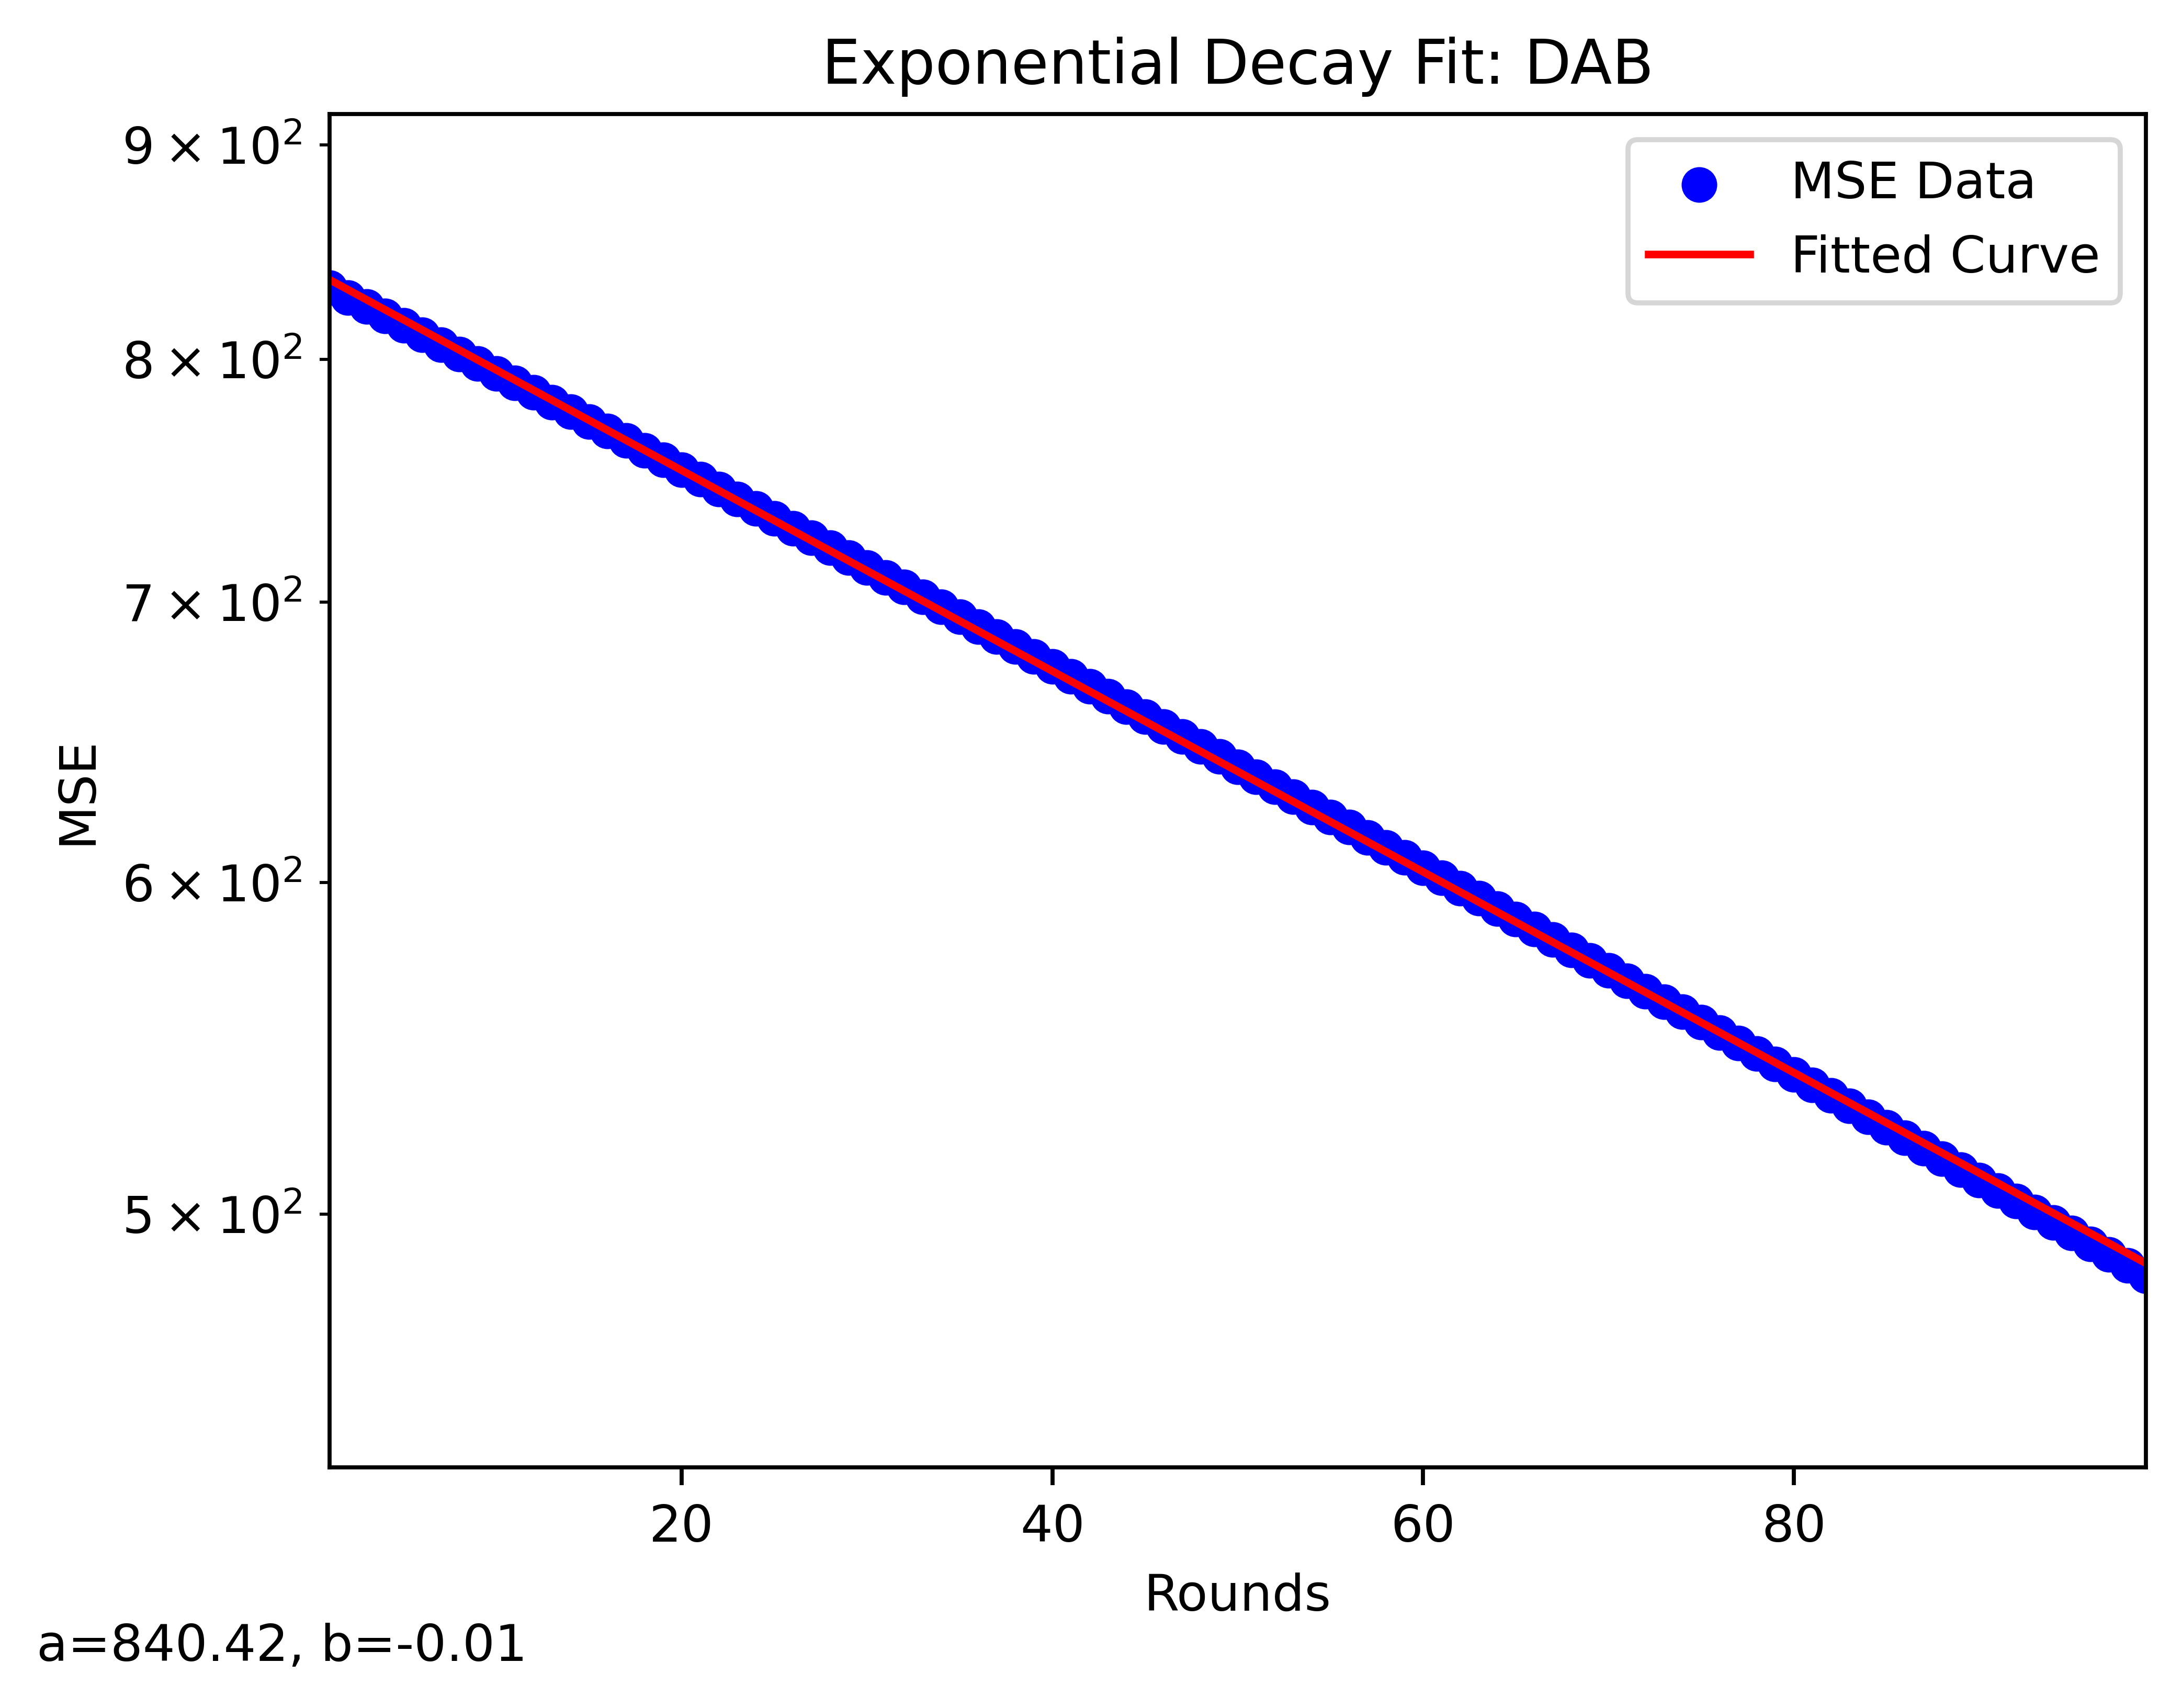
\includegraphics[width=\linewidth]{figures/Simulation_outcomes/StarGraph/DAB/DAB_modelfitting_rounds_99_model_1.png}
%     \caption{Exponential Decay Fit: DAB}
%     \label{fig:dabStarModelFit}
% \end{figure}


\textbf{Push-Pull Sum Algorithm and Adaptive Threshold Push-Pull Sum Algorithm}: Both push-pull-based protocols exhibit steep MSE reductions early on, as seen in the sharp downward trends in the log-log plot. The PPS algorithm outperforms the ATPPS algorithm, as it reduces MSE faster and reaches lower MSE values sooner (as of round 45) before the graph plateaus. Figures \ref{fig:ppsStarModelFit} and \ref{fig:atppsStarModelFit} show the fitted curves for the MSE data of the PPS and ATPPS load balancing algorithms respectively. The best-fit model for the MSE data of the PPS load balancing algorithm for the rounds 10 to 45 follows the equation $MSE=29794.60*e^{-1.39*x}$. The rounds 10 to 45 show the steepest decay and for that reason been fitted to exponential regression model. The decay rate of -1.39 indicates a very fast error reduction in the network, especially if compared to the DAB load balancing algorithms ability to reduce the error for star graph. The ATPPS load balancing algorithms MSE data fits best with the exponential model following the equation $MSE_r=9329.40*e^{-1.05*r}$ between the rounds 18 to 60. In star graphs, the central node dominates communication, and the load balancing heavily depends on that node. Threshold adjustments may not sufficiently impact performance under these conditions.

Overall the scenario is similiar to the complete graph, where the DAB reduces the error exponential with a very slow rate, while the push-pull based algorithms perform a very fast error reduction. This behaviour is captured in the heat map of figure \ref{fig:stargraphslopes}. While the DAB load balancing algorithm reduces the error in average per region $-3.75 \pm 0.55$, the push-pull based algorithms exhibit a error reduction of -92 for the first 10 rounds. The slopes approach zero in the middle and end regions, implying almost negligible MSE reduction in later stages. This is due to the fact that the network already is balanced to a degree where the MSE will not improve significantly further for later rounds. Both algorithms converge early and maintain a near-steady state afterward. The DAB load balancing algorithms deterministic nature and lack of adaptability lead to slower convergence and less effective load balancing, as reflected in its consistently shallow slopes.

% \begin{figure}[H]
%     \centering
%     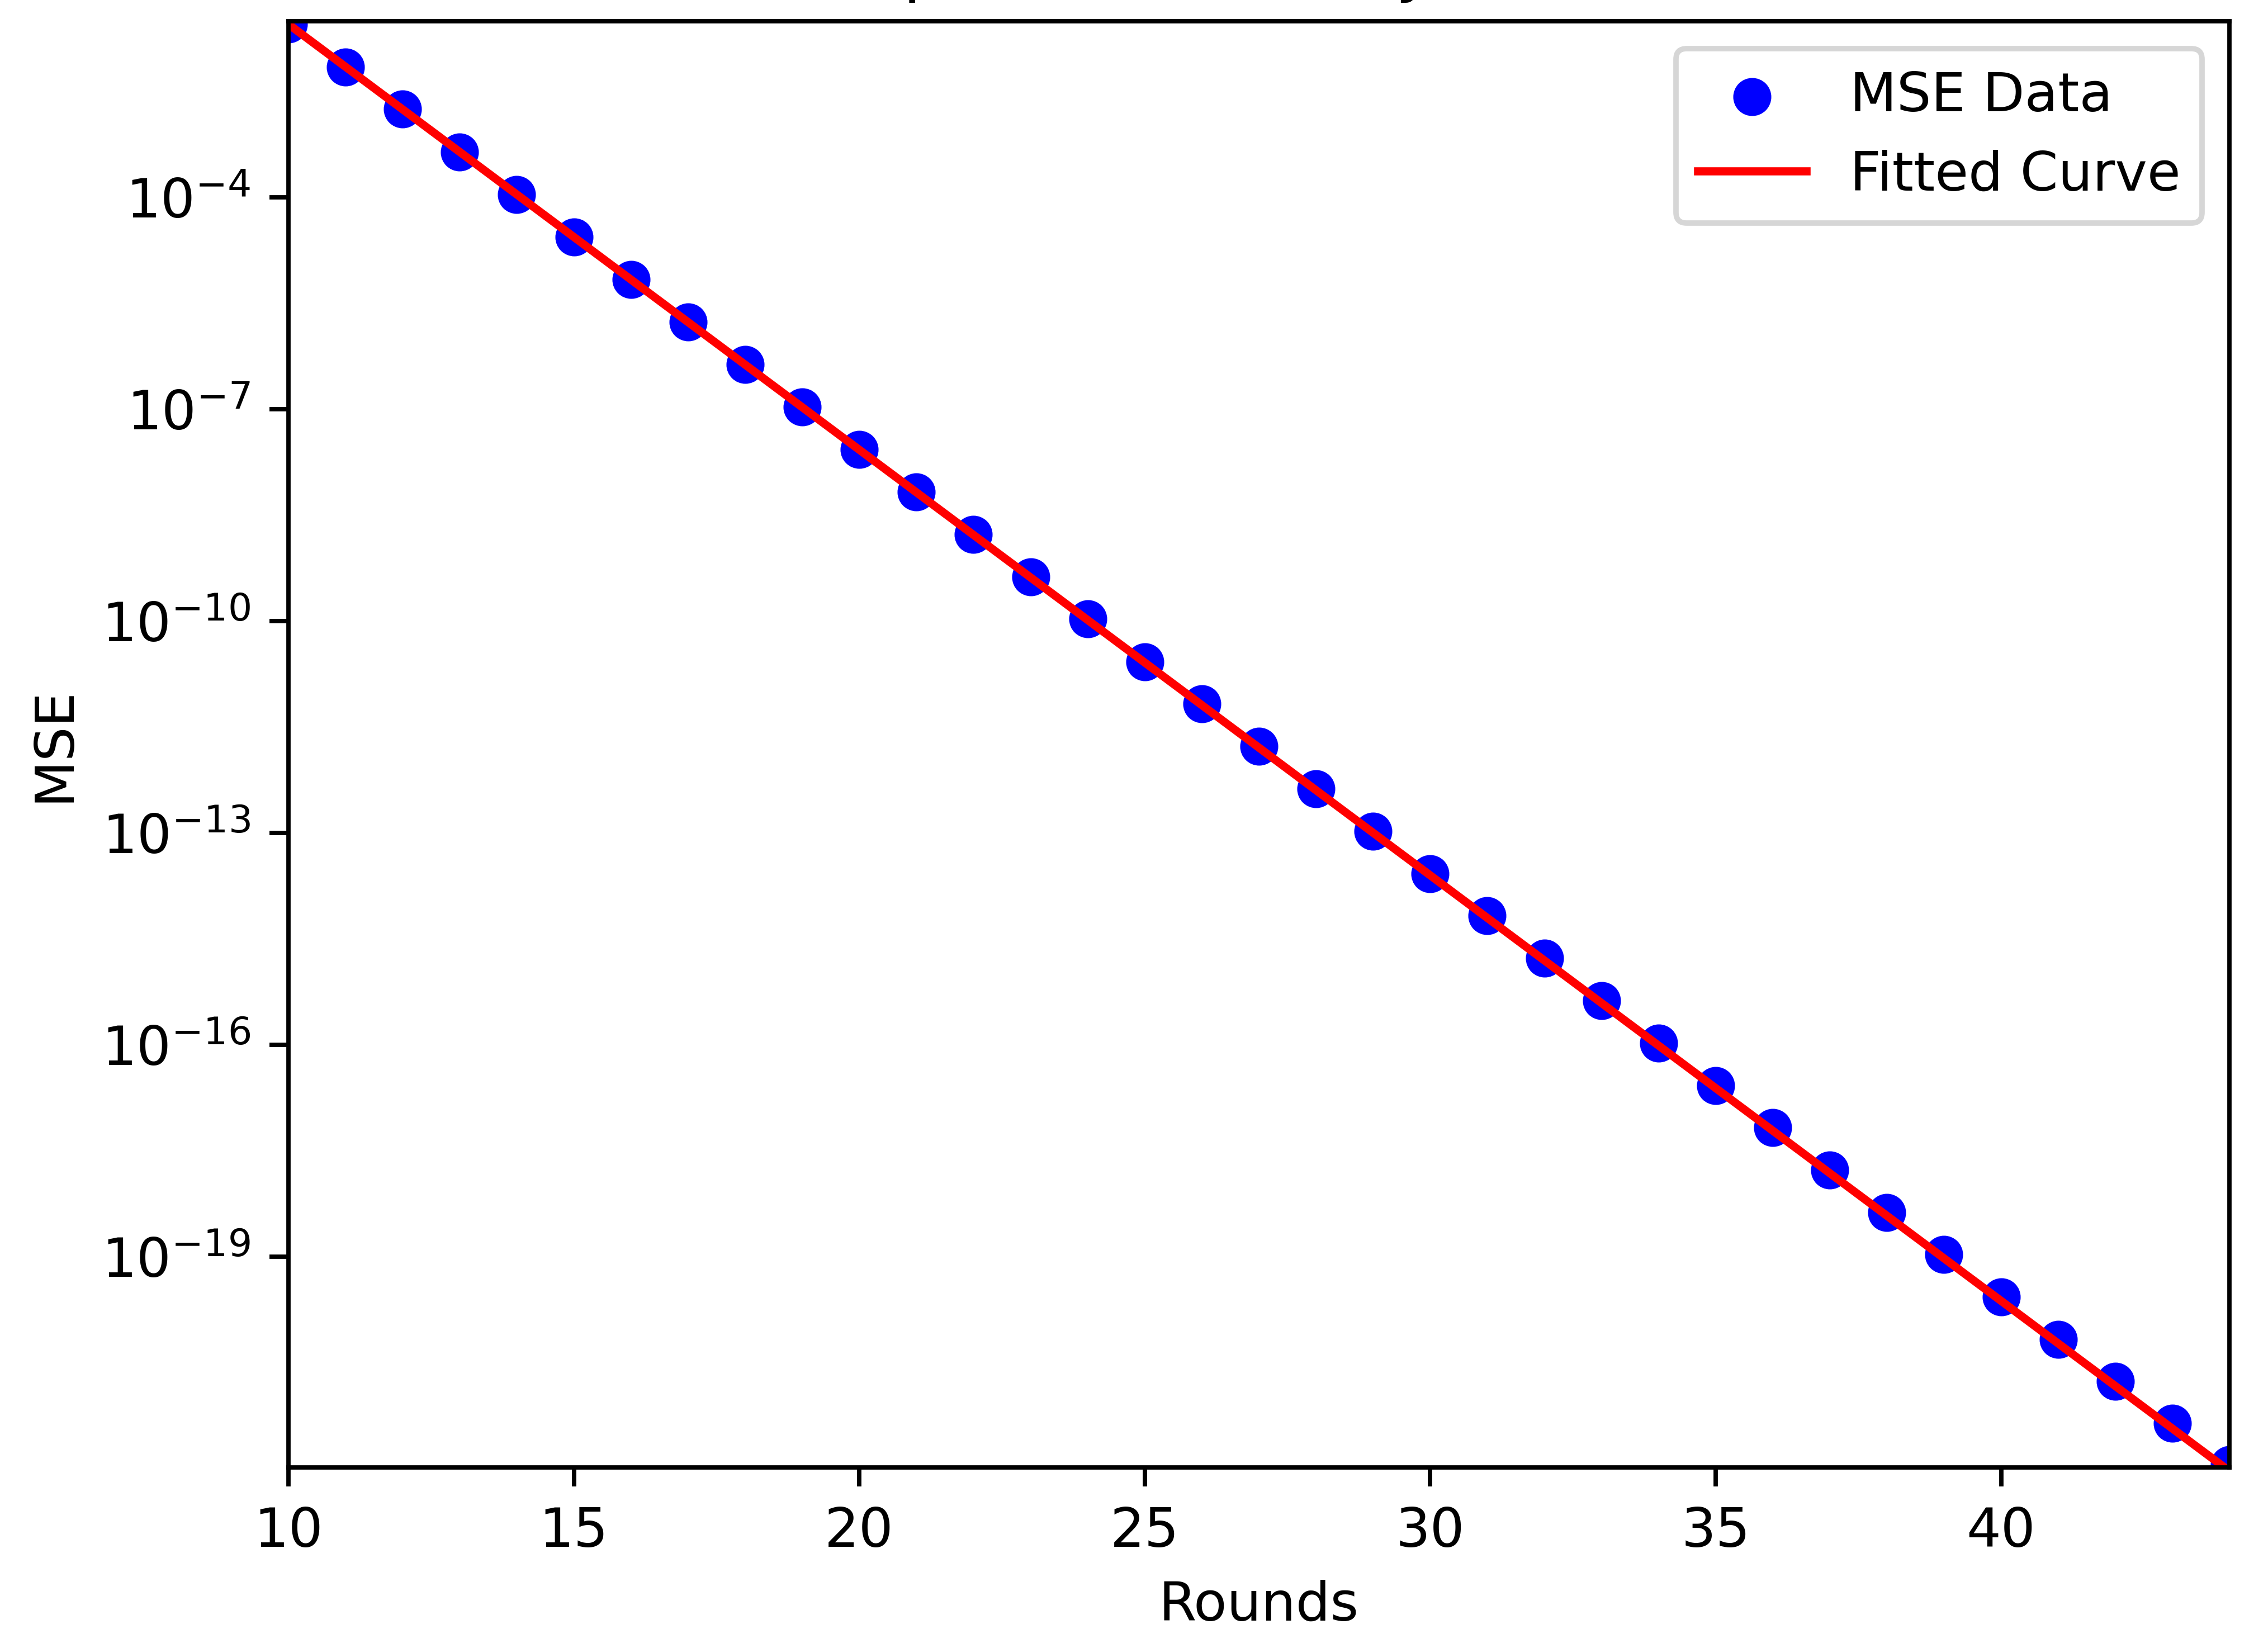
\includegraphics[width=\linewidth]{figures/Simulation_outcomes/StarGraph/PPS/PPS_modelfitting_rounds_44_model_1.png}
%     \caption{Exponential Decay Fit: PPS}
%     \label{fig:ppsStarModelFit}
% \end{figure}

% \begin{figure}[H]
%     \centering
%     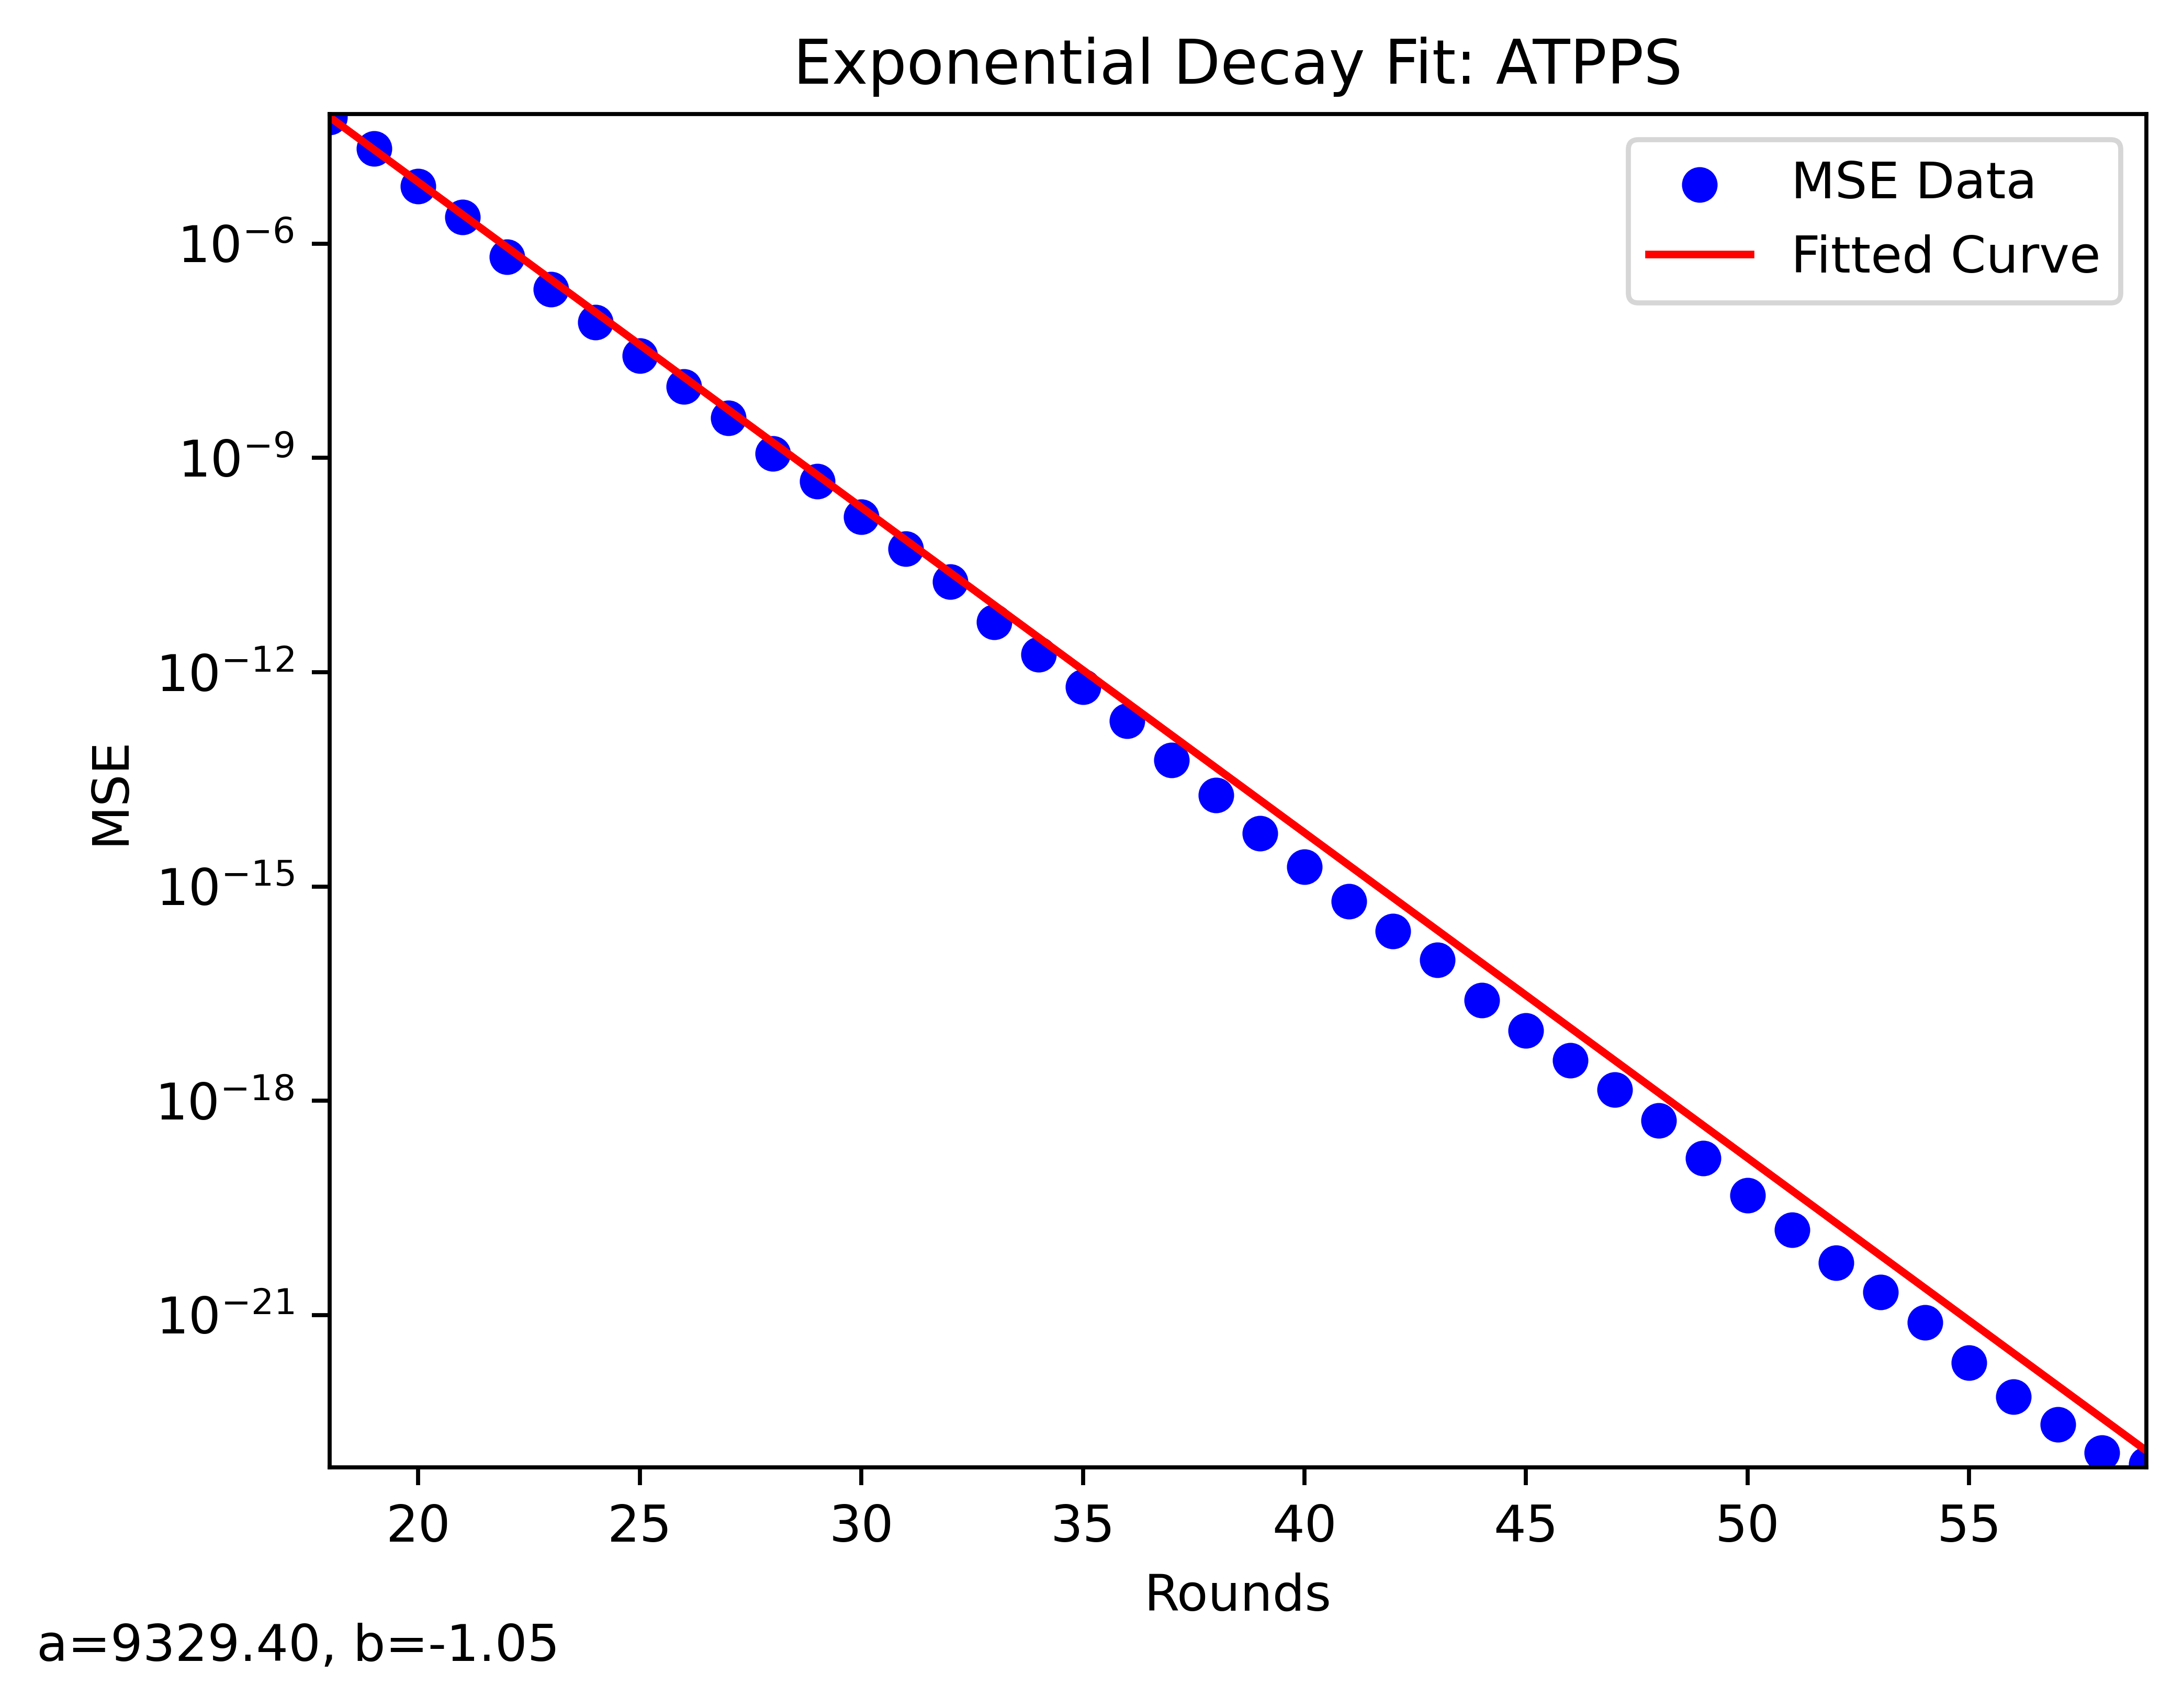
\includegraphics[width=\linewidth]{figures/Simulation_outcomes/StarGraph/ATPPS/ATPPS_modelfitting_rounds_59_model_1.png}
%     \caption{Exponential Decay Fit: ATPPS}
%     \label{fig:atppsStarModelFit}
% \end{figure}

% \begin{figure}
%     \centering
%     \scalebox{0.8}{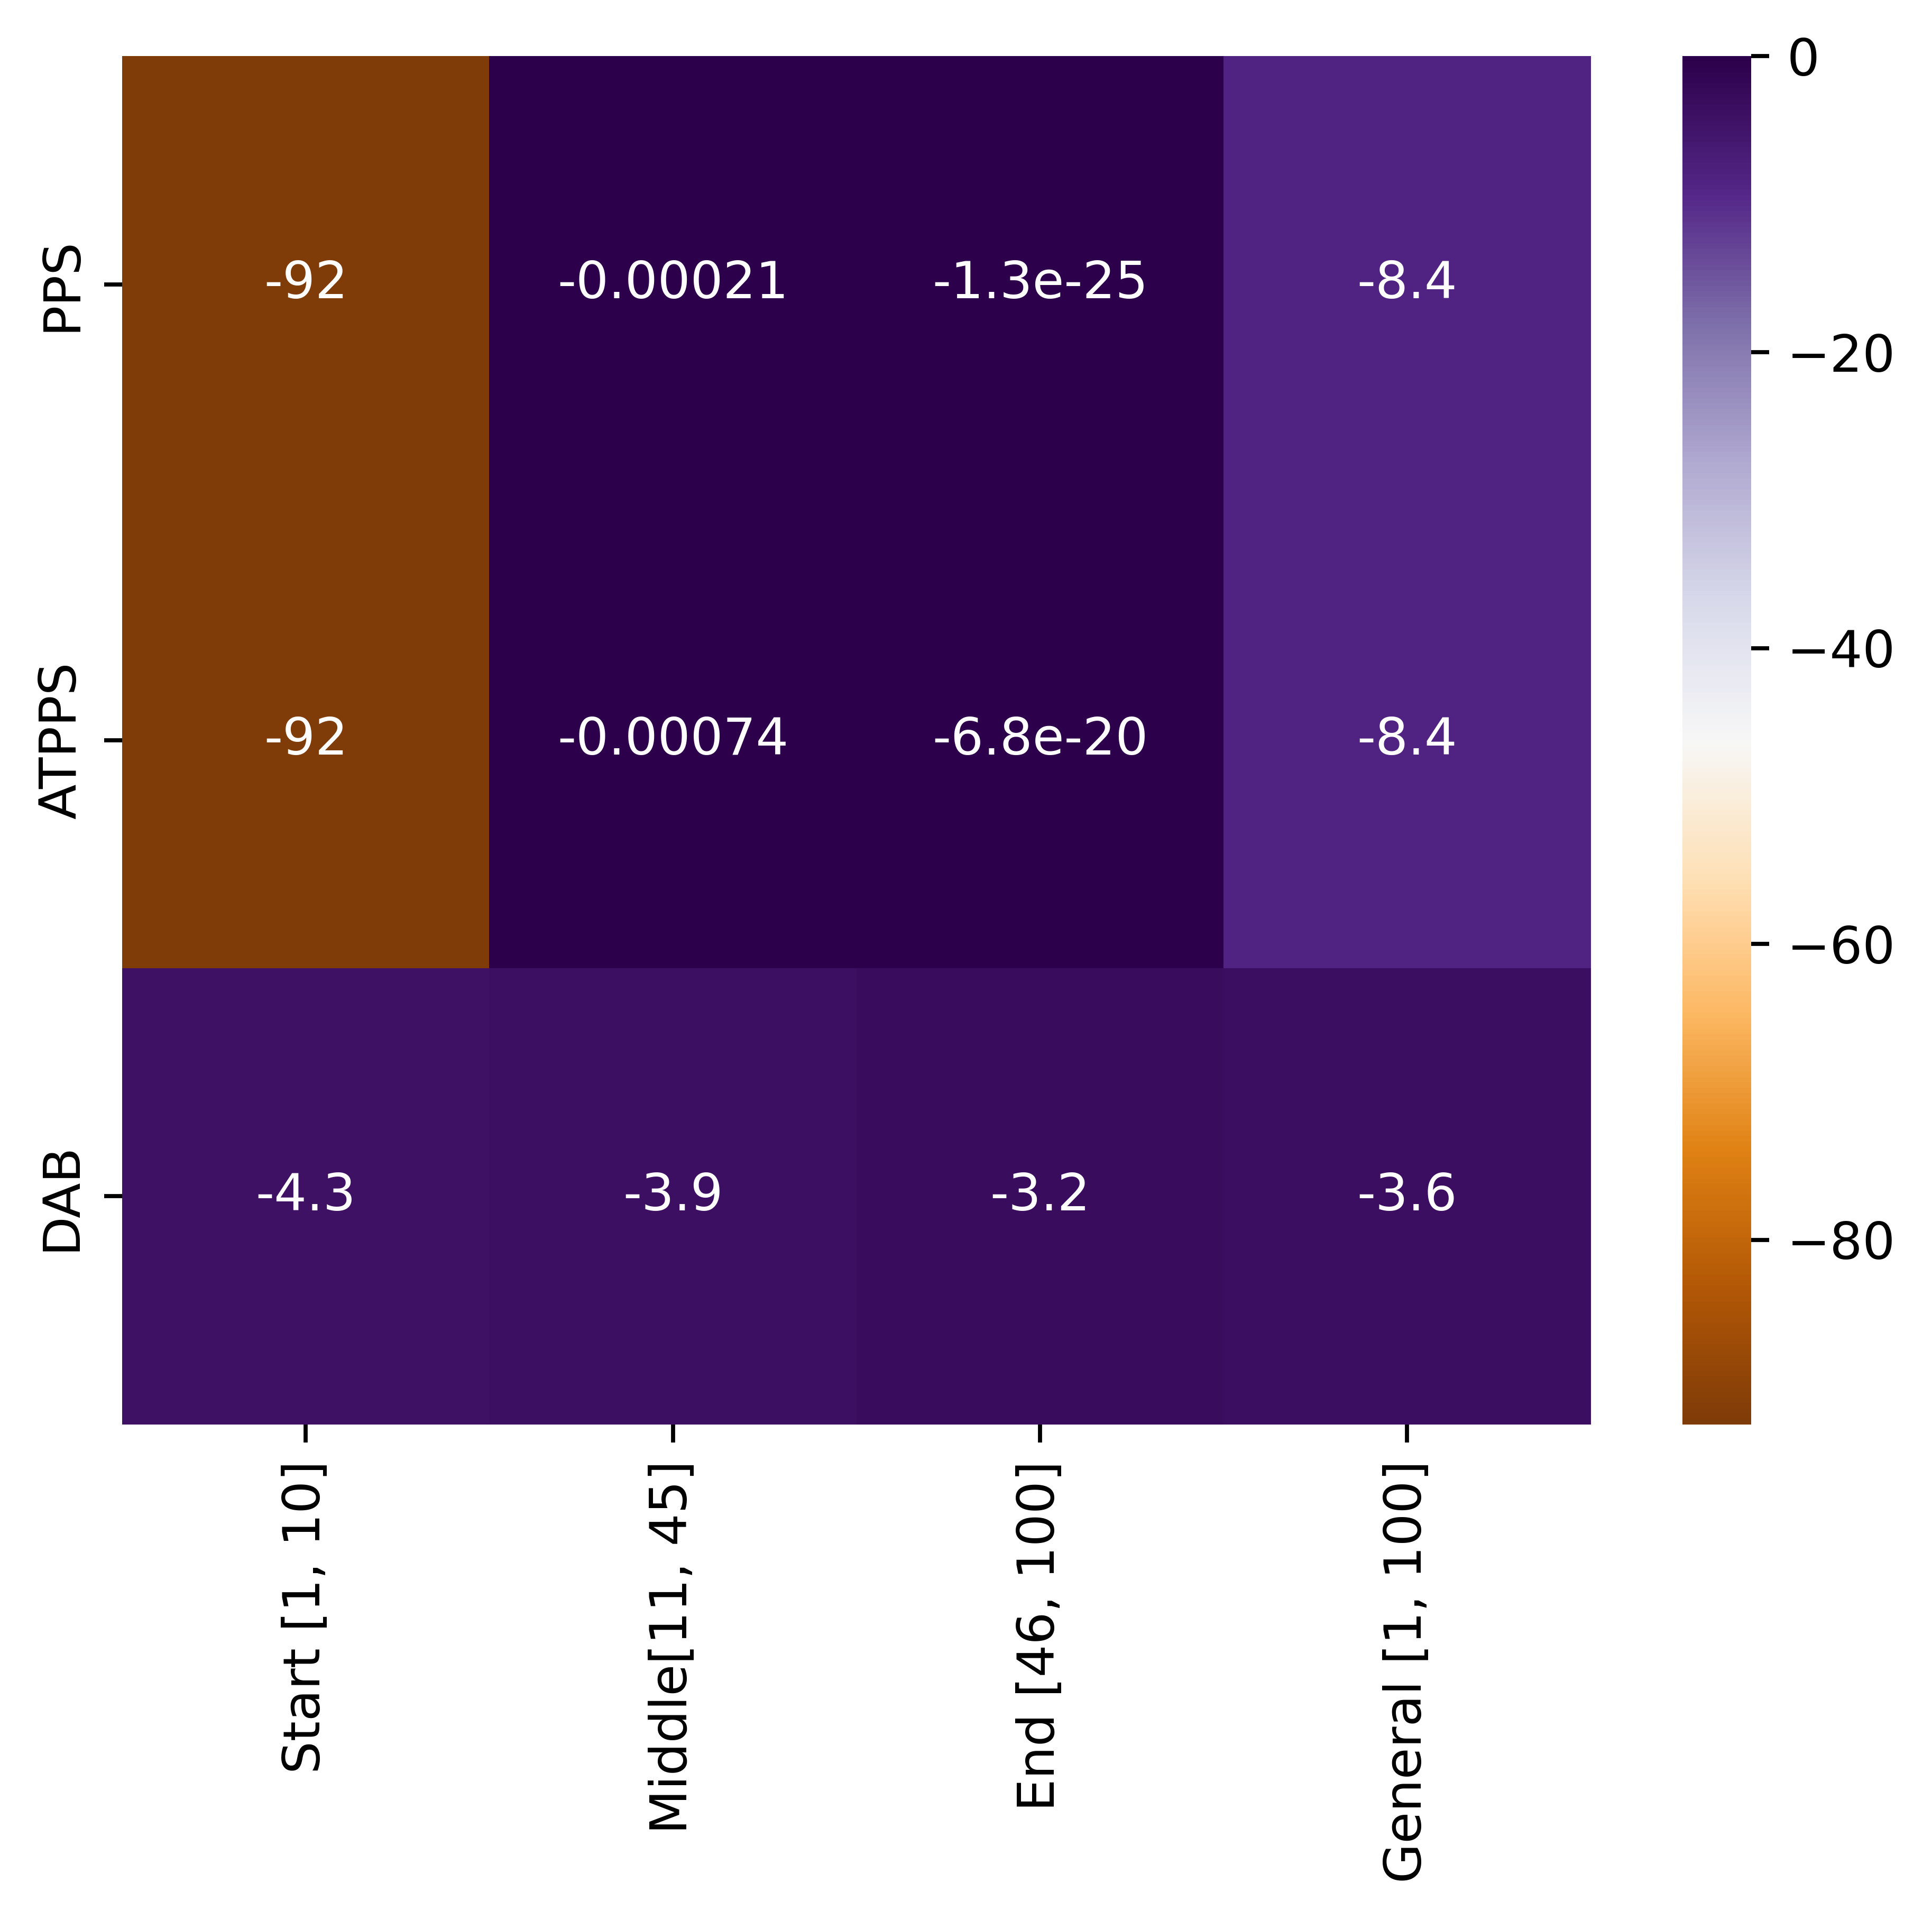
\includegraphics{figures/Simulation_outcomes/StarGraph/DAB_vs_PPS_vs_ATPPS_slopesheatmap_100rounds.png}}
%     \caption{Star Graph: heat map of slopes per region}
%     \label{fig:stargraphslopes}
% \end{figure}

\section{Ring Graph}\label{sec:ringgraph}
The DAB curve in figure \ref{fig:ringgraphMSEperRoundLogLog} shows the steepest decline in error in the first few rounds of the simulation. The slope of the first 10 rounds is -84 for the DAB curve compared to -82 for each PPS-based algorithm as depicted in figure \ref{fig:ringgraphslopes}. The near-overlap of PPS and ATPPS across the 100 rounds of simulation indicates that the adaptive mechanism provides limited additional benefit in a ring graph topology, where load balancing is already well-facilitated by regular communication patterns. In a ring topology, each node only has access to its two neighbors. The adaptive threshold mechanism relies on meaningful differences in load between nodes to trigger exchanges, but in a ring, local differences might not vary significantly enough to make the threshold mechanism advantageous for each neighborhood. In the classic PPS, every node communicates with its neighbors in every round. This constant exchange ensures rapid propagation of load updates. The adaptive threshold might reduce some of these exchanges, but in a ring graph, where the diameter is large, reducing communication might delay convergence rather than improve it. Thus, the threshold mechanism could counteract its own benefits. The DAB algorithm functions way better in this scenario, since it always interacts with the optimal partner to exchange loads. The randomness benefit vanishes for a network topology where each node only has two neighbors, and a deterministic approach actually performs better.

The MSE data of each algorithms simulations were fitted to the polynomial regression model with degree of 4 each. The best-fit model for the DAB MSE data for the rounds 10 to 60 follow the equation: $MSE_r=1.72*10^{-05}-0.0023r+ 0.19r^{2}-5.99r^{3}+114.83r^{4}$ (figure \ref{fig:dabRingModelFit}). The intercept ($a_0$ term) is very close to zero, meaning the starting MSE value is almost entirely determined by higher-order terms. The small negative coefficient of the $a_1$-term indicates a slight initial linear decrease in MSE as rounds progress, contributing a modest downward slope. The positive quadratic term ($a_2$ term) suggests a curving trend. This term provides more flexibility to account for changes in the decay rate of the MSE early in the rounds. The cubic term ($a_3$ term) adds further curvature but with a decreasing influence with proceeding rounds. It could model an inflection point in the MSE trend. The large positive coefficient of the cubic term ($a-4$ term) reflects the steep decay behavior of MSE over a significant portion of the range. A similiar behaviour is shown for the PPS and ATPPS curves which are fitted for the model: $MSE_r= 2.99*10^{-05}-0.5*10^{-2}r + 0.32r^{2} -9.68r^{3} + 166.30r{4}$ (figure \ref{fig:ppsRingModelFit})for the PPS and the model: $3.04*10^{-05}-0.5*10^{-2}r + 0.32r^{2}-9.64r^{3}+161.86r^{5}$ (figure \ref{fig:atppsRingModelFit})for the ATPPS.

% \begin{figure}[h]
%     \centering
%     \scalebox{0.5}{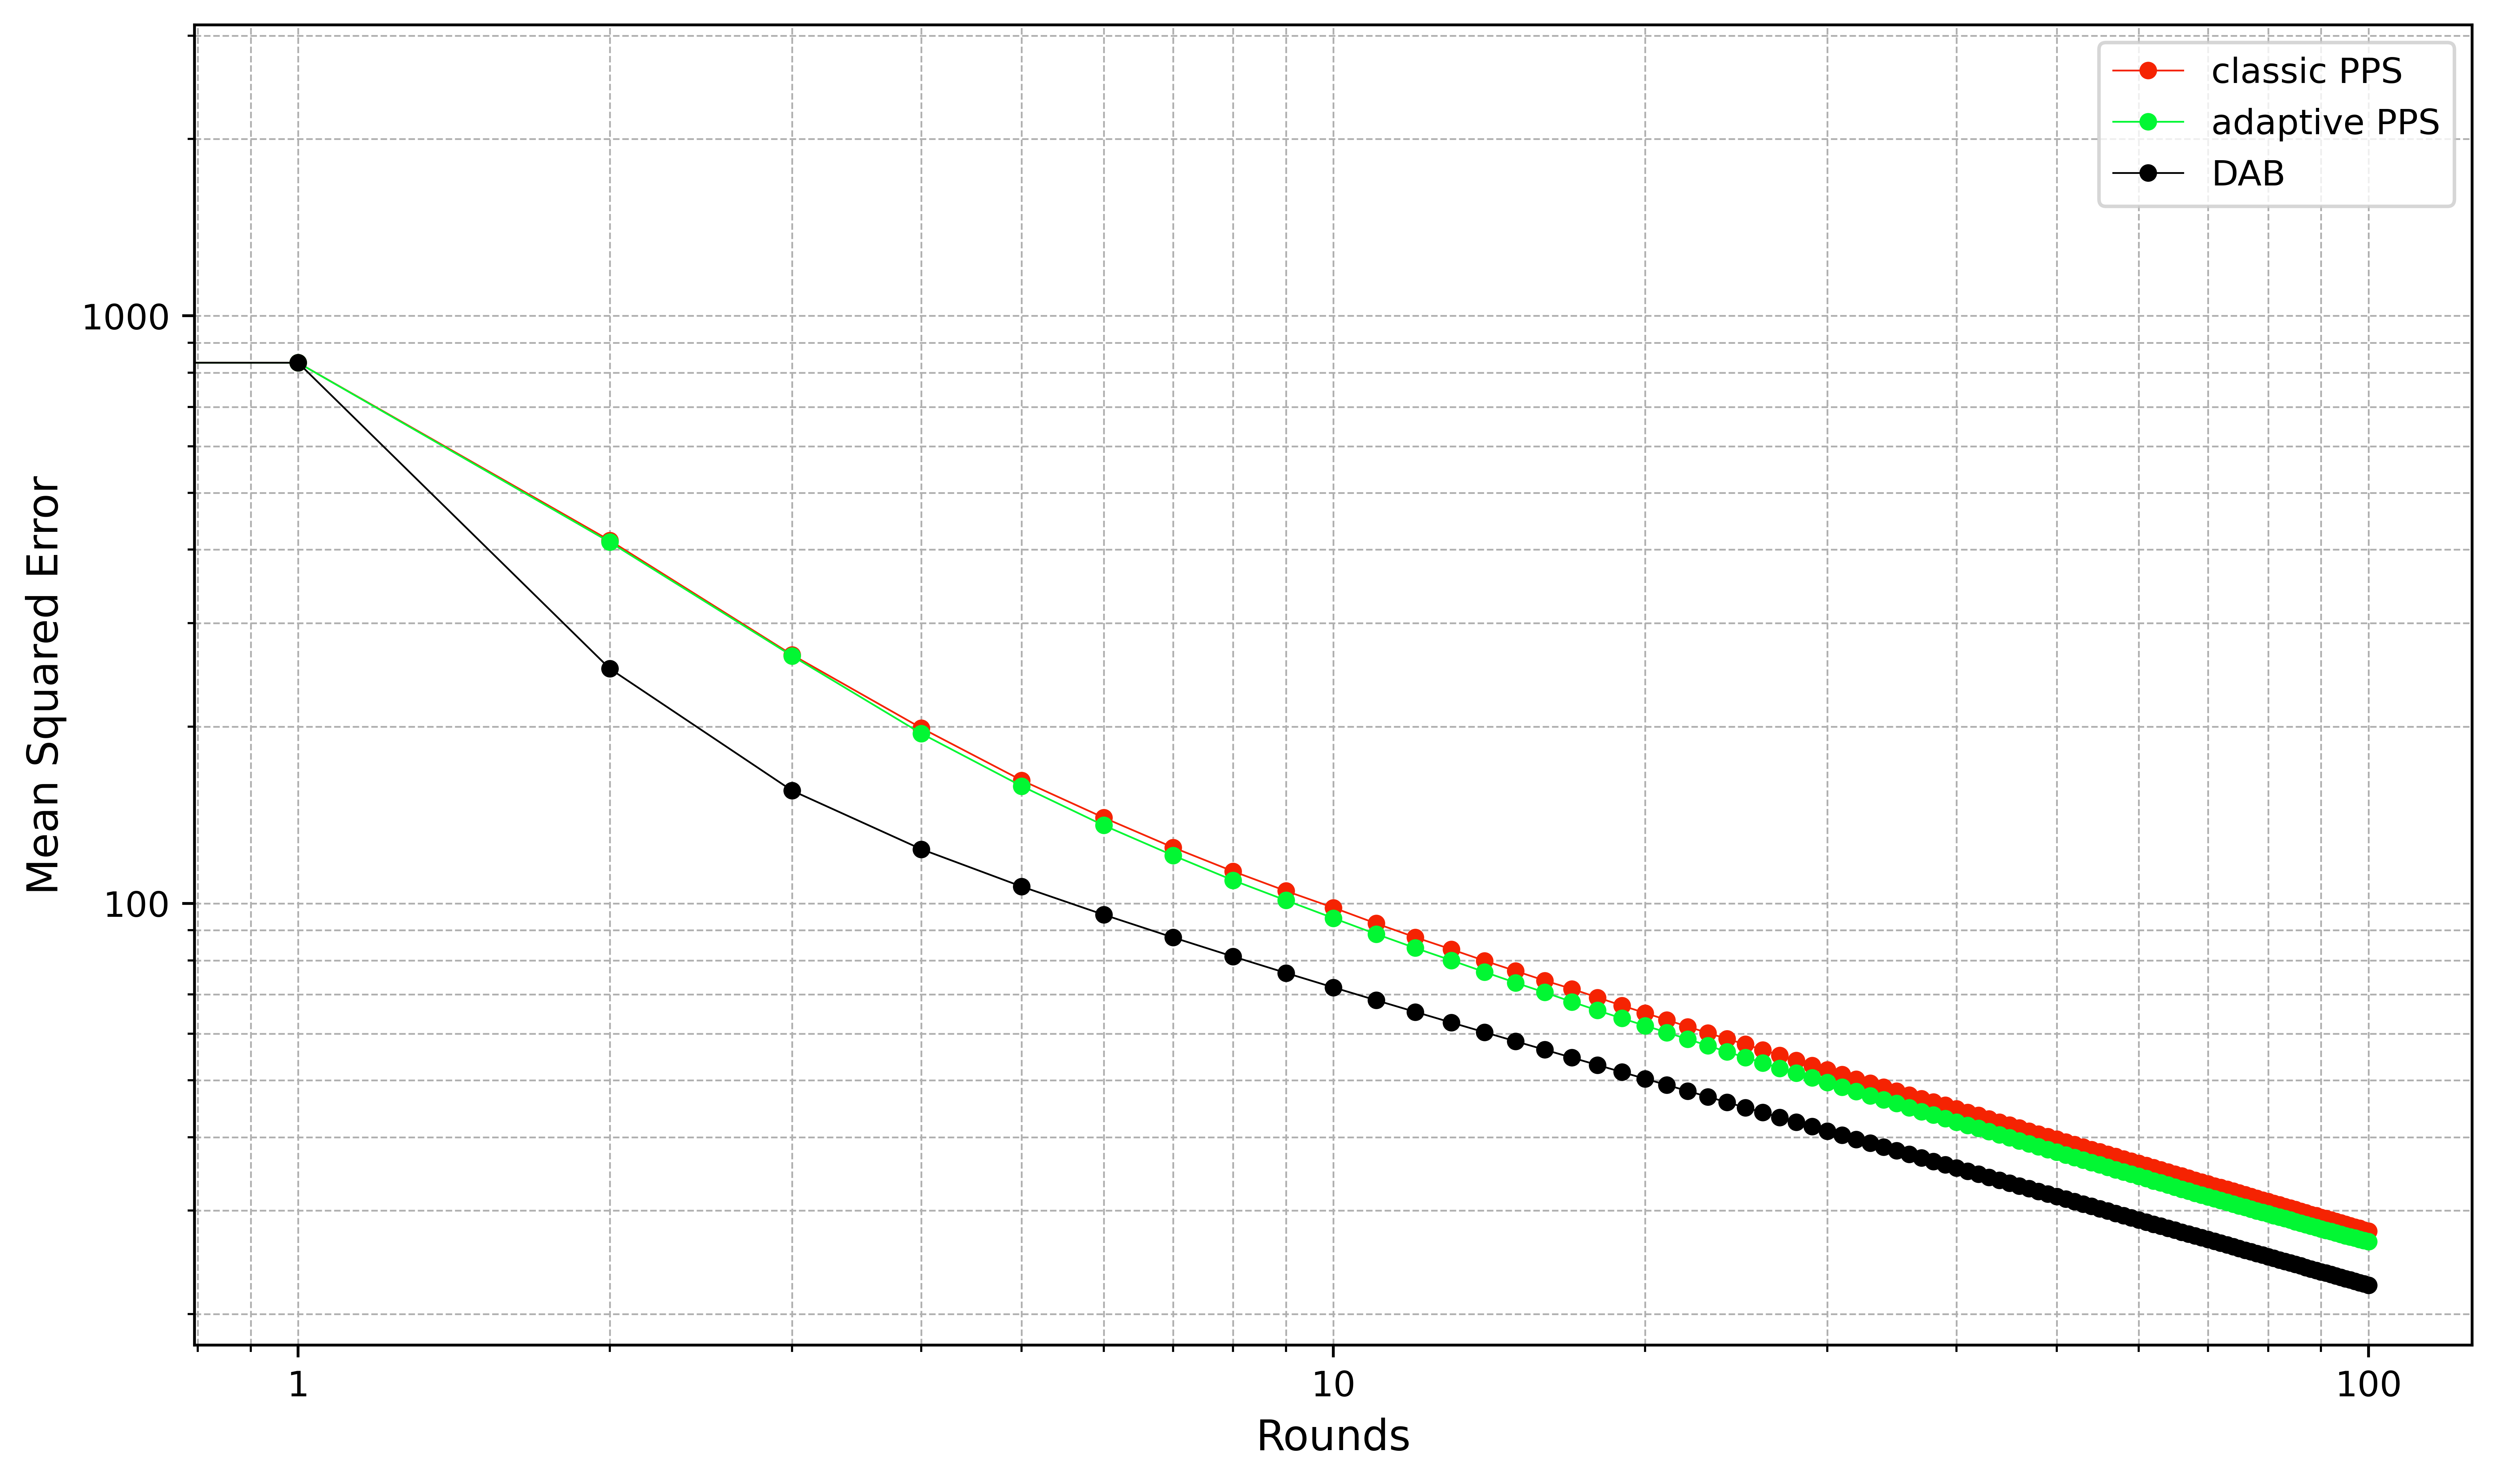
\includegraphics{figures/Simulation_outcomes/RingGraph/DAB_vs_PPS_RG_r100_n1024_averaged_loglog.png}}
%     \caption{Ring Graph: mean squared error per rounds (log-log)}
%     \label{fig:ringgraphMSEperRoundLogLog}
% \end{figure}

% \begin{figure}[H]
%     \centering
%     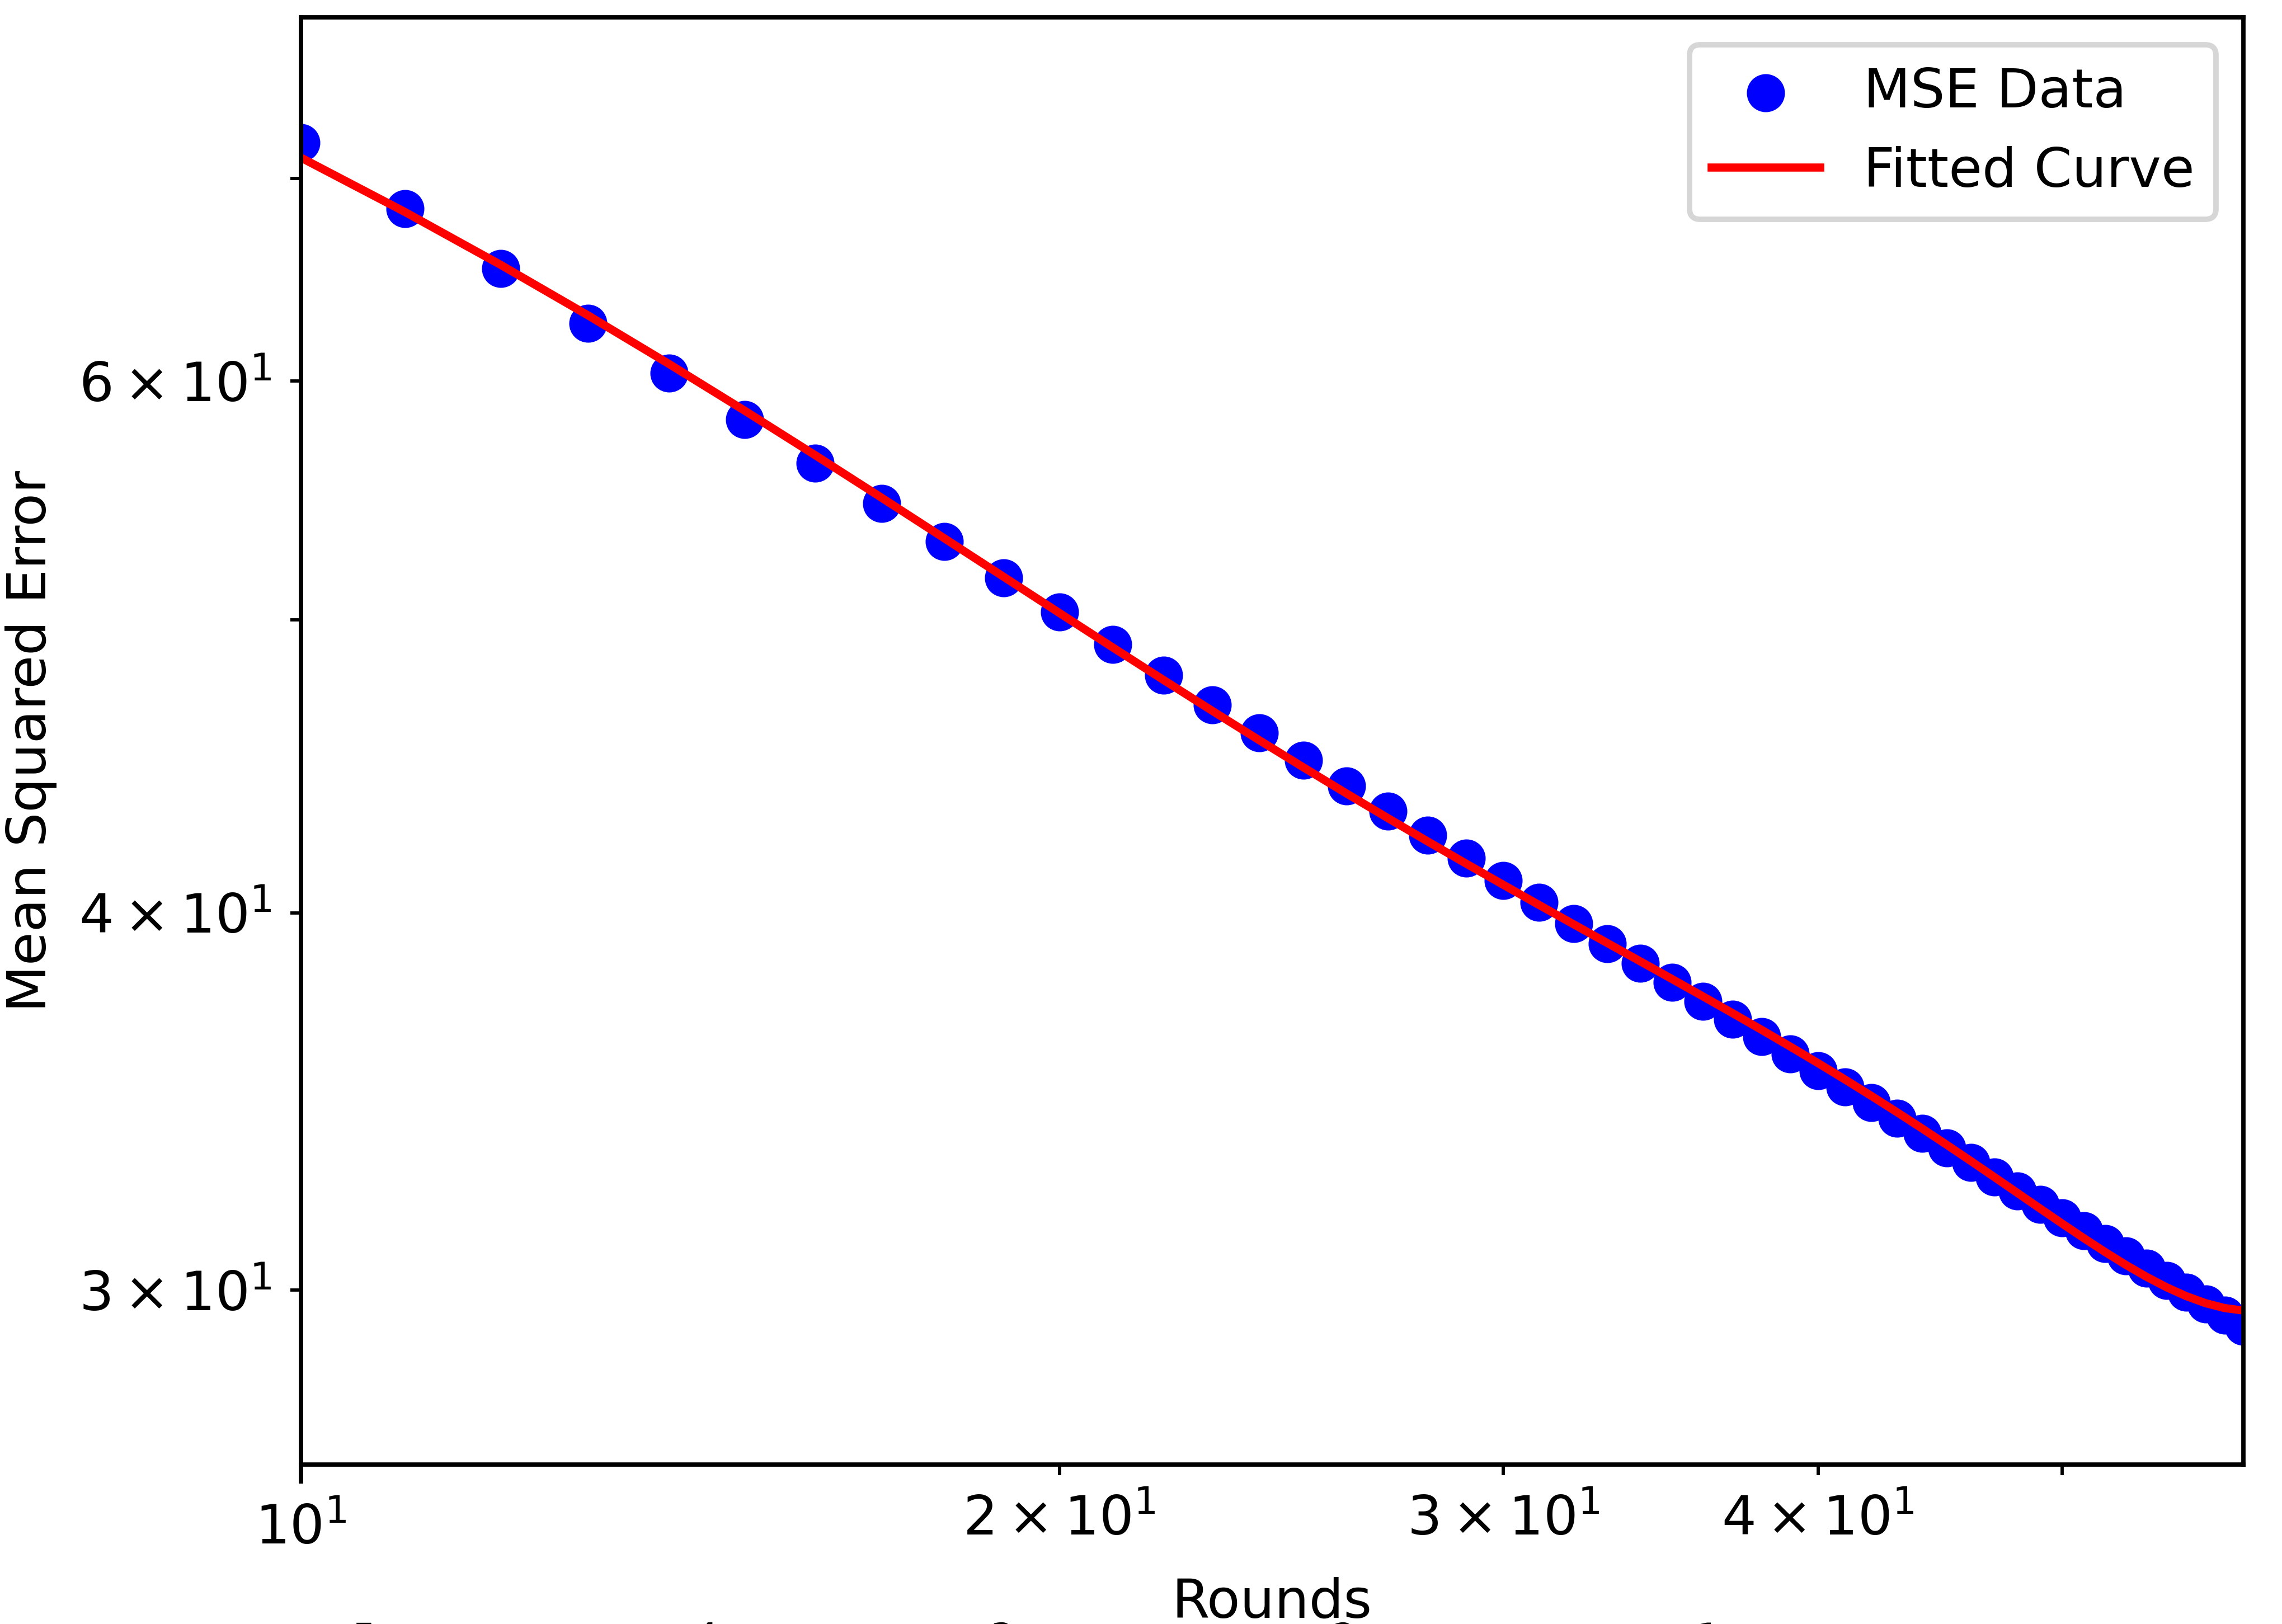
\includegraphics[width=\linewidth]{figures/Simulation_outcomes/RingGraph/DAB/DAB_modelfitting_rounds_59_model_2.png}
%     \caption{Polynomial Regression Fit: DAB}
%     \label{fig:dabRingModelFit}
% \end{figure}

%\begin{figure}[H]
%    \centering
%    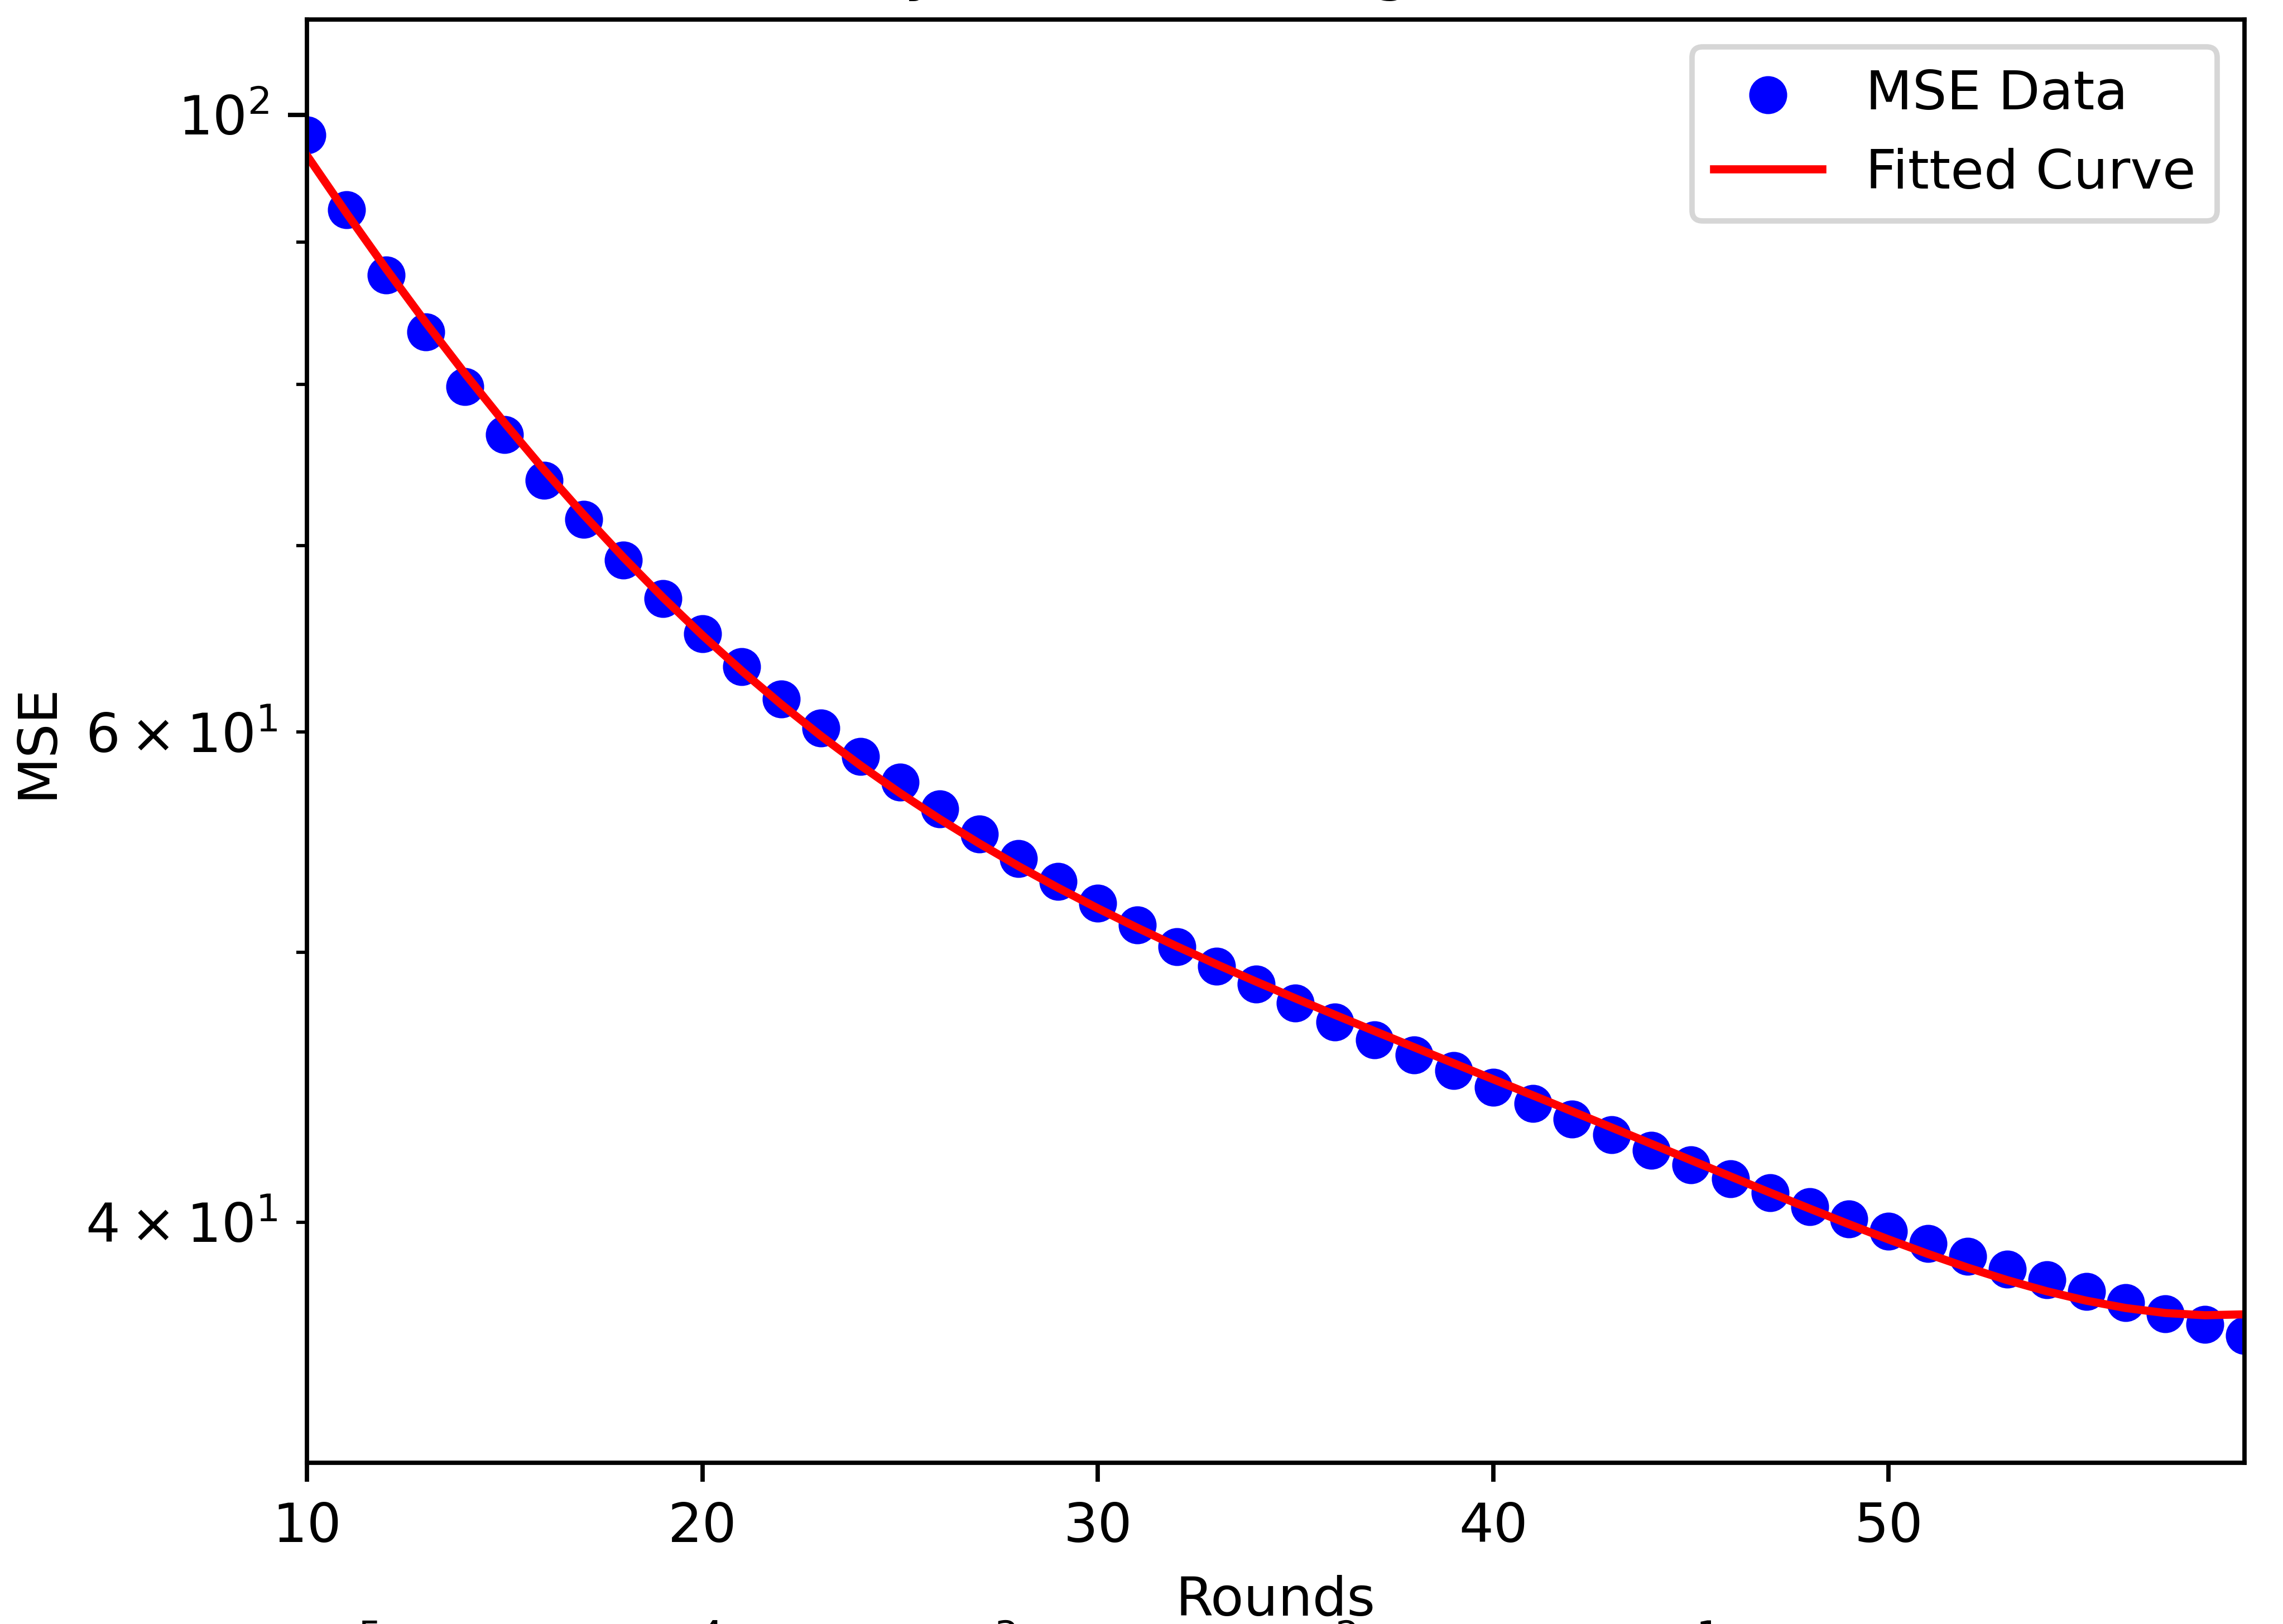
\includegraphics[width=\linewidth]{figures/Simulation_outcomes/RingGraph/PPS/PPS_modelfitting_rounds_59_model_2.png}
%    \caption{Polynomial Regression Fit: PPS}
%    \label{fig:ppsRingModelFit}
%\end{figure}

% \begin{figure}[H]
%     \centering
%     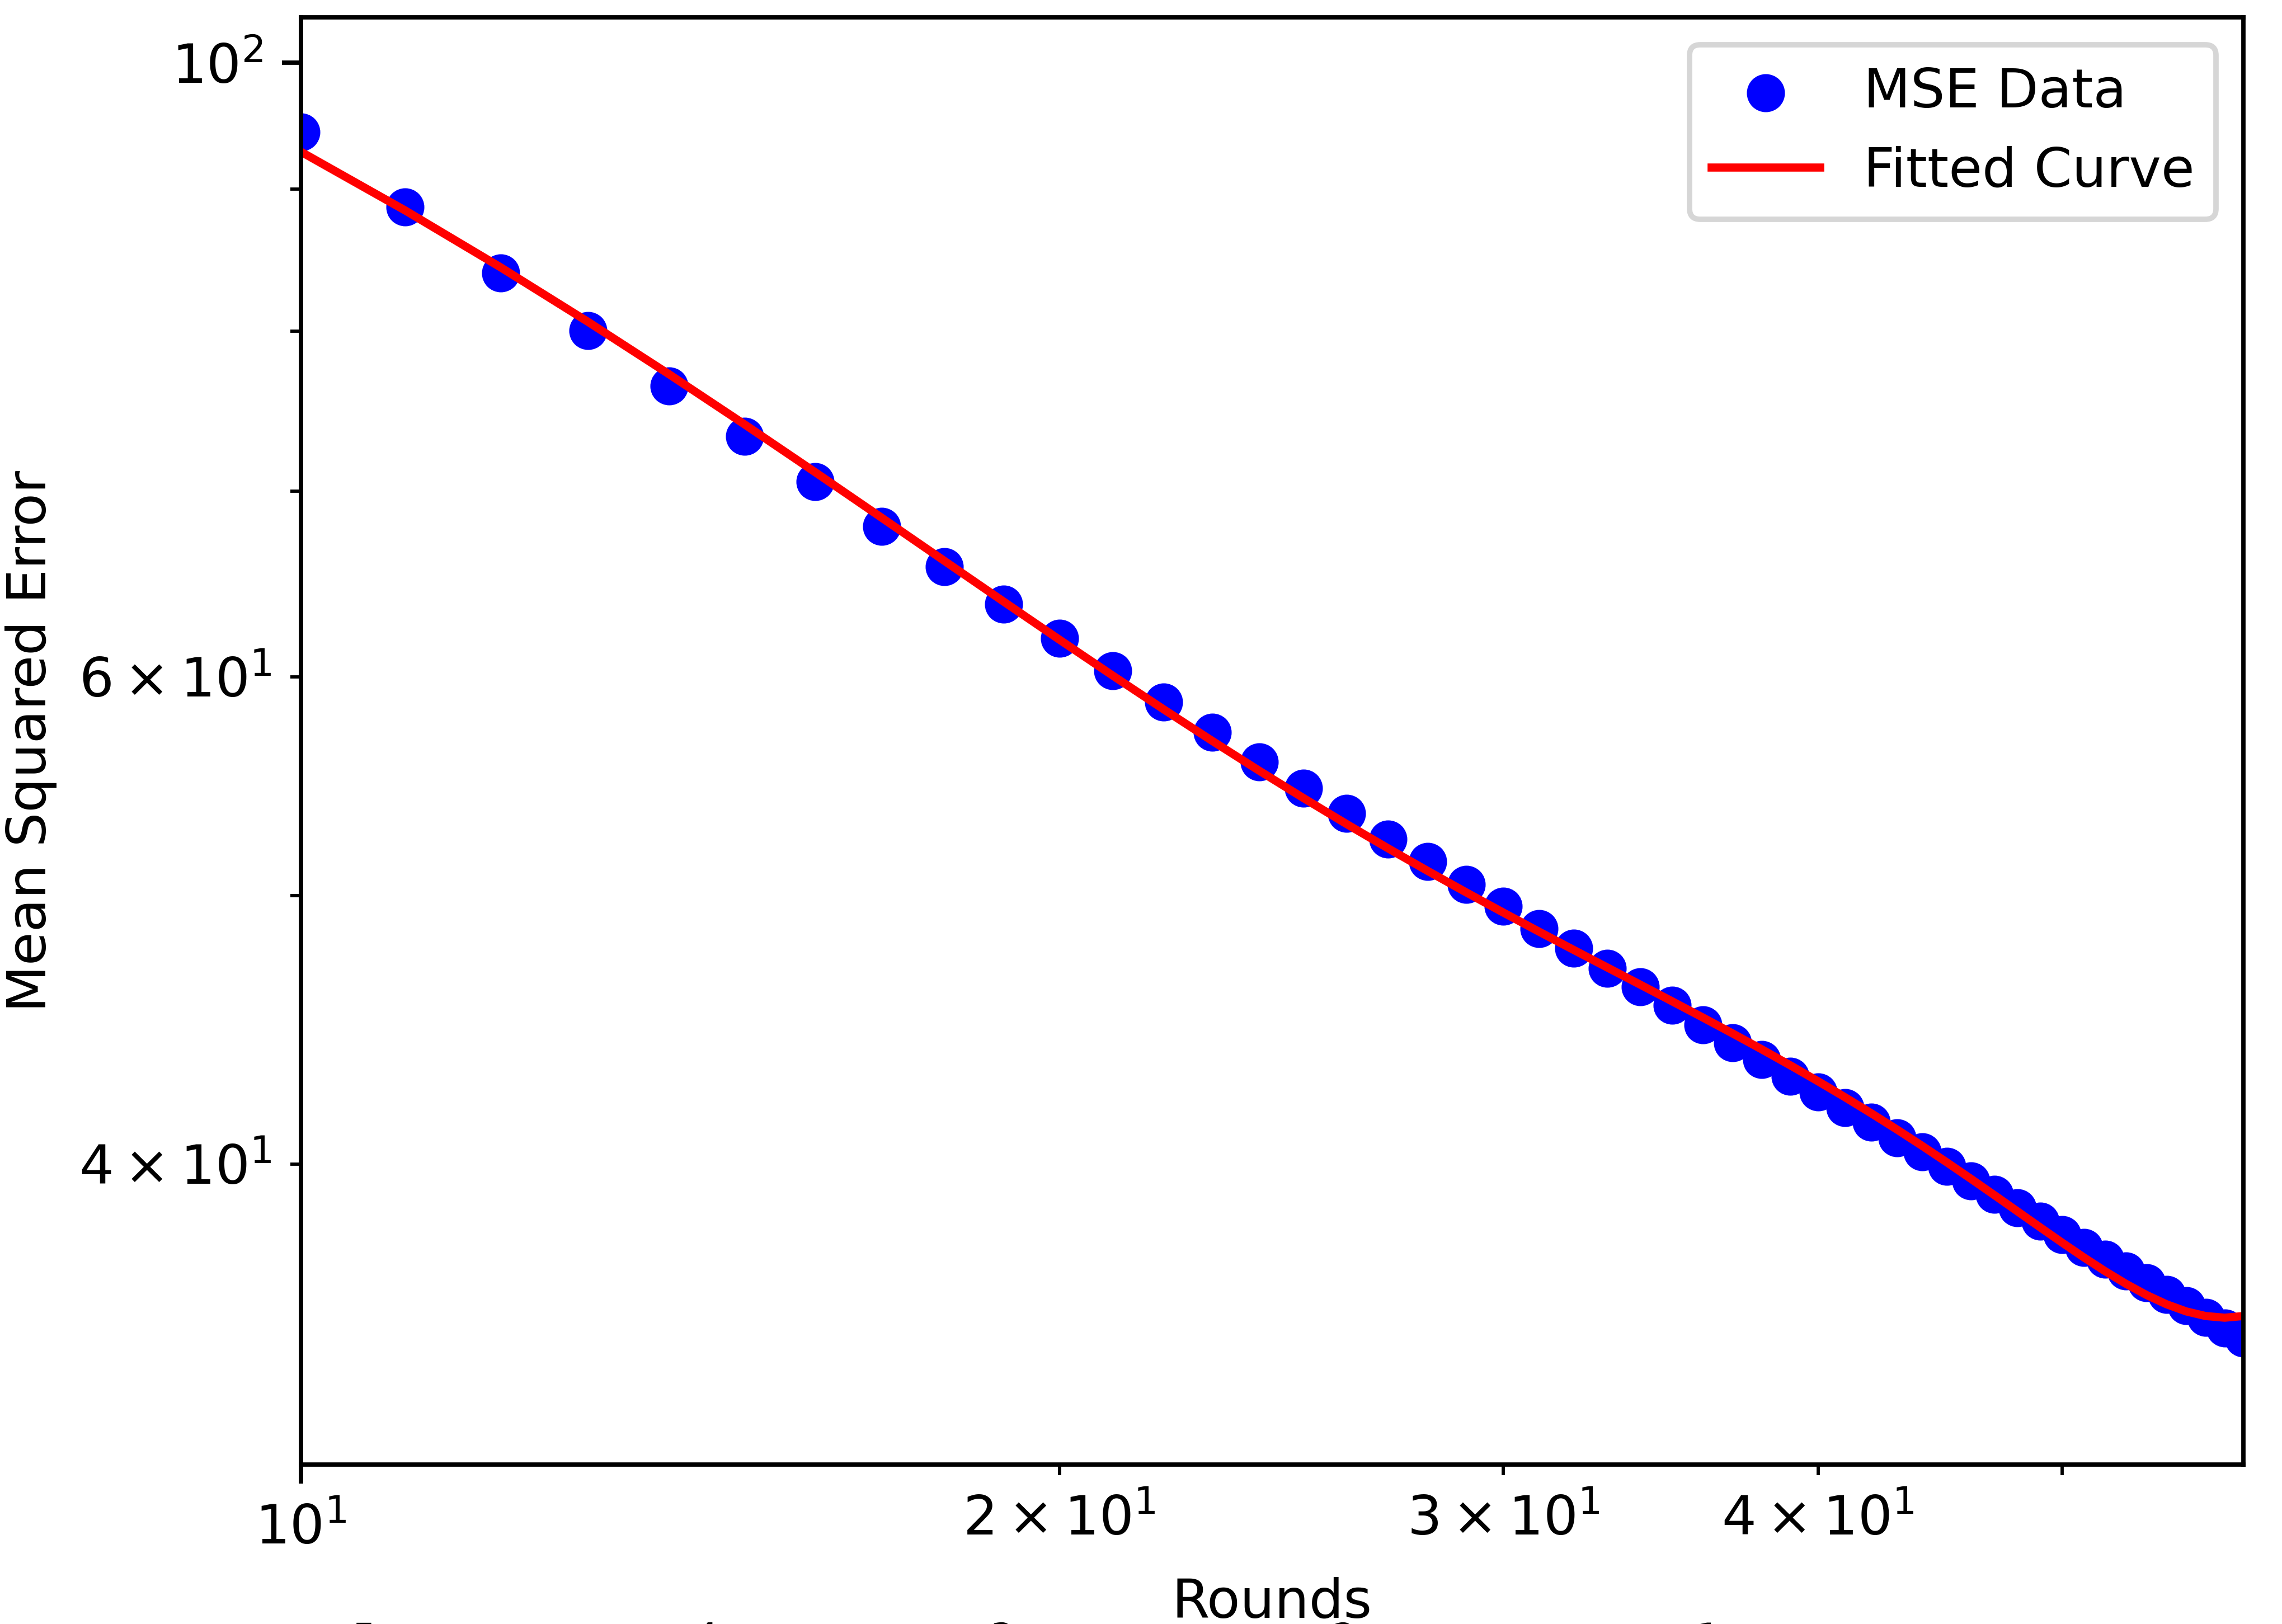
\includegraphics[width=\linewidth]{figures/Simulation_outcomes/RingGraph/ATPPS/ATPPS_modelfitting_rounds_59_model_2.png}
%     \caption{Polynomial Regression Fit: ATPPS}
%     \label{fig:atppsRingModelFit}
% \end{figure}

% \begin{figure}
%     \centering
%     \scalebox{0.8}{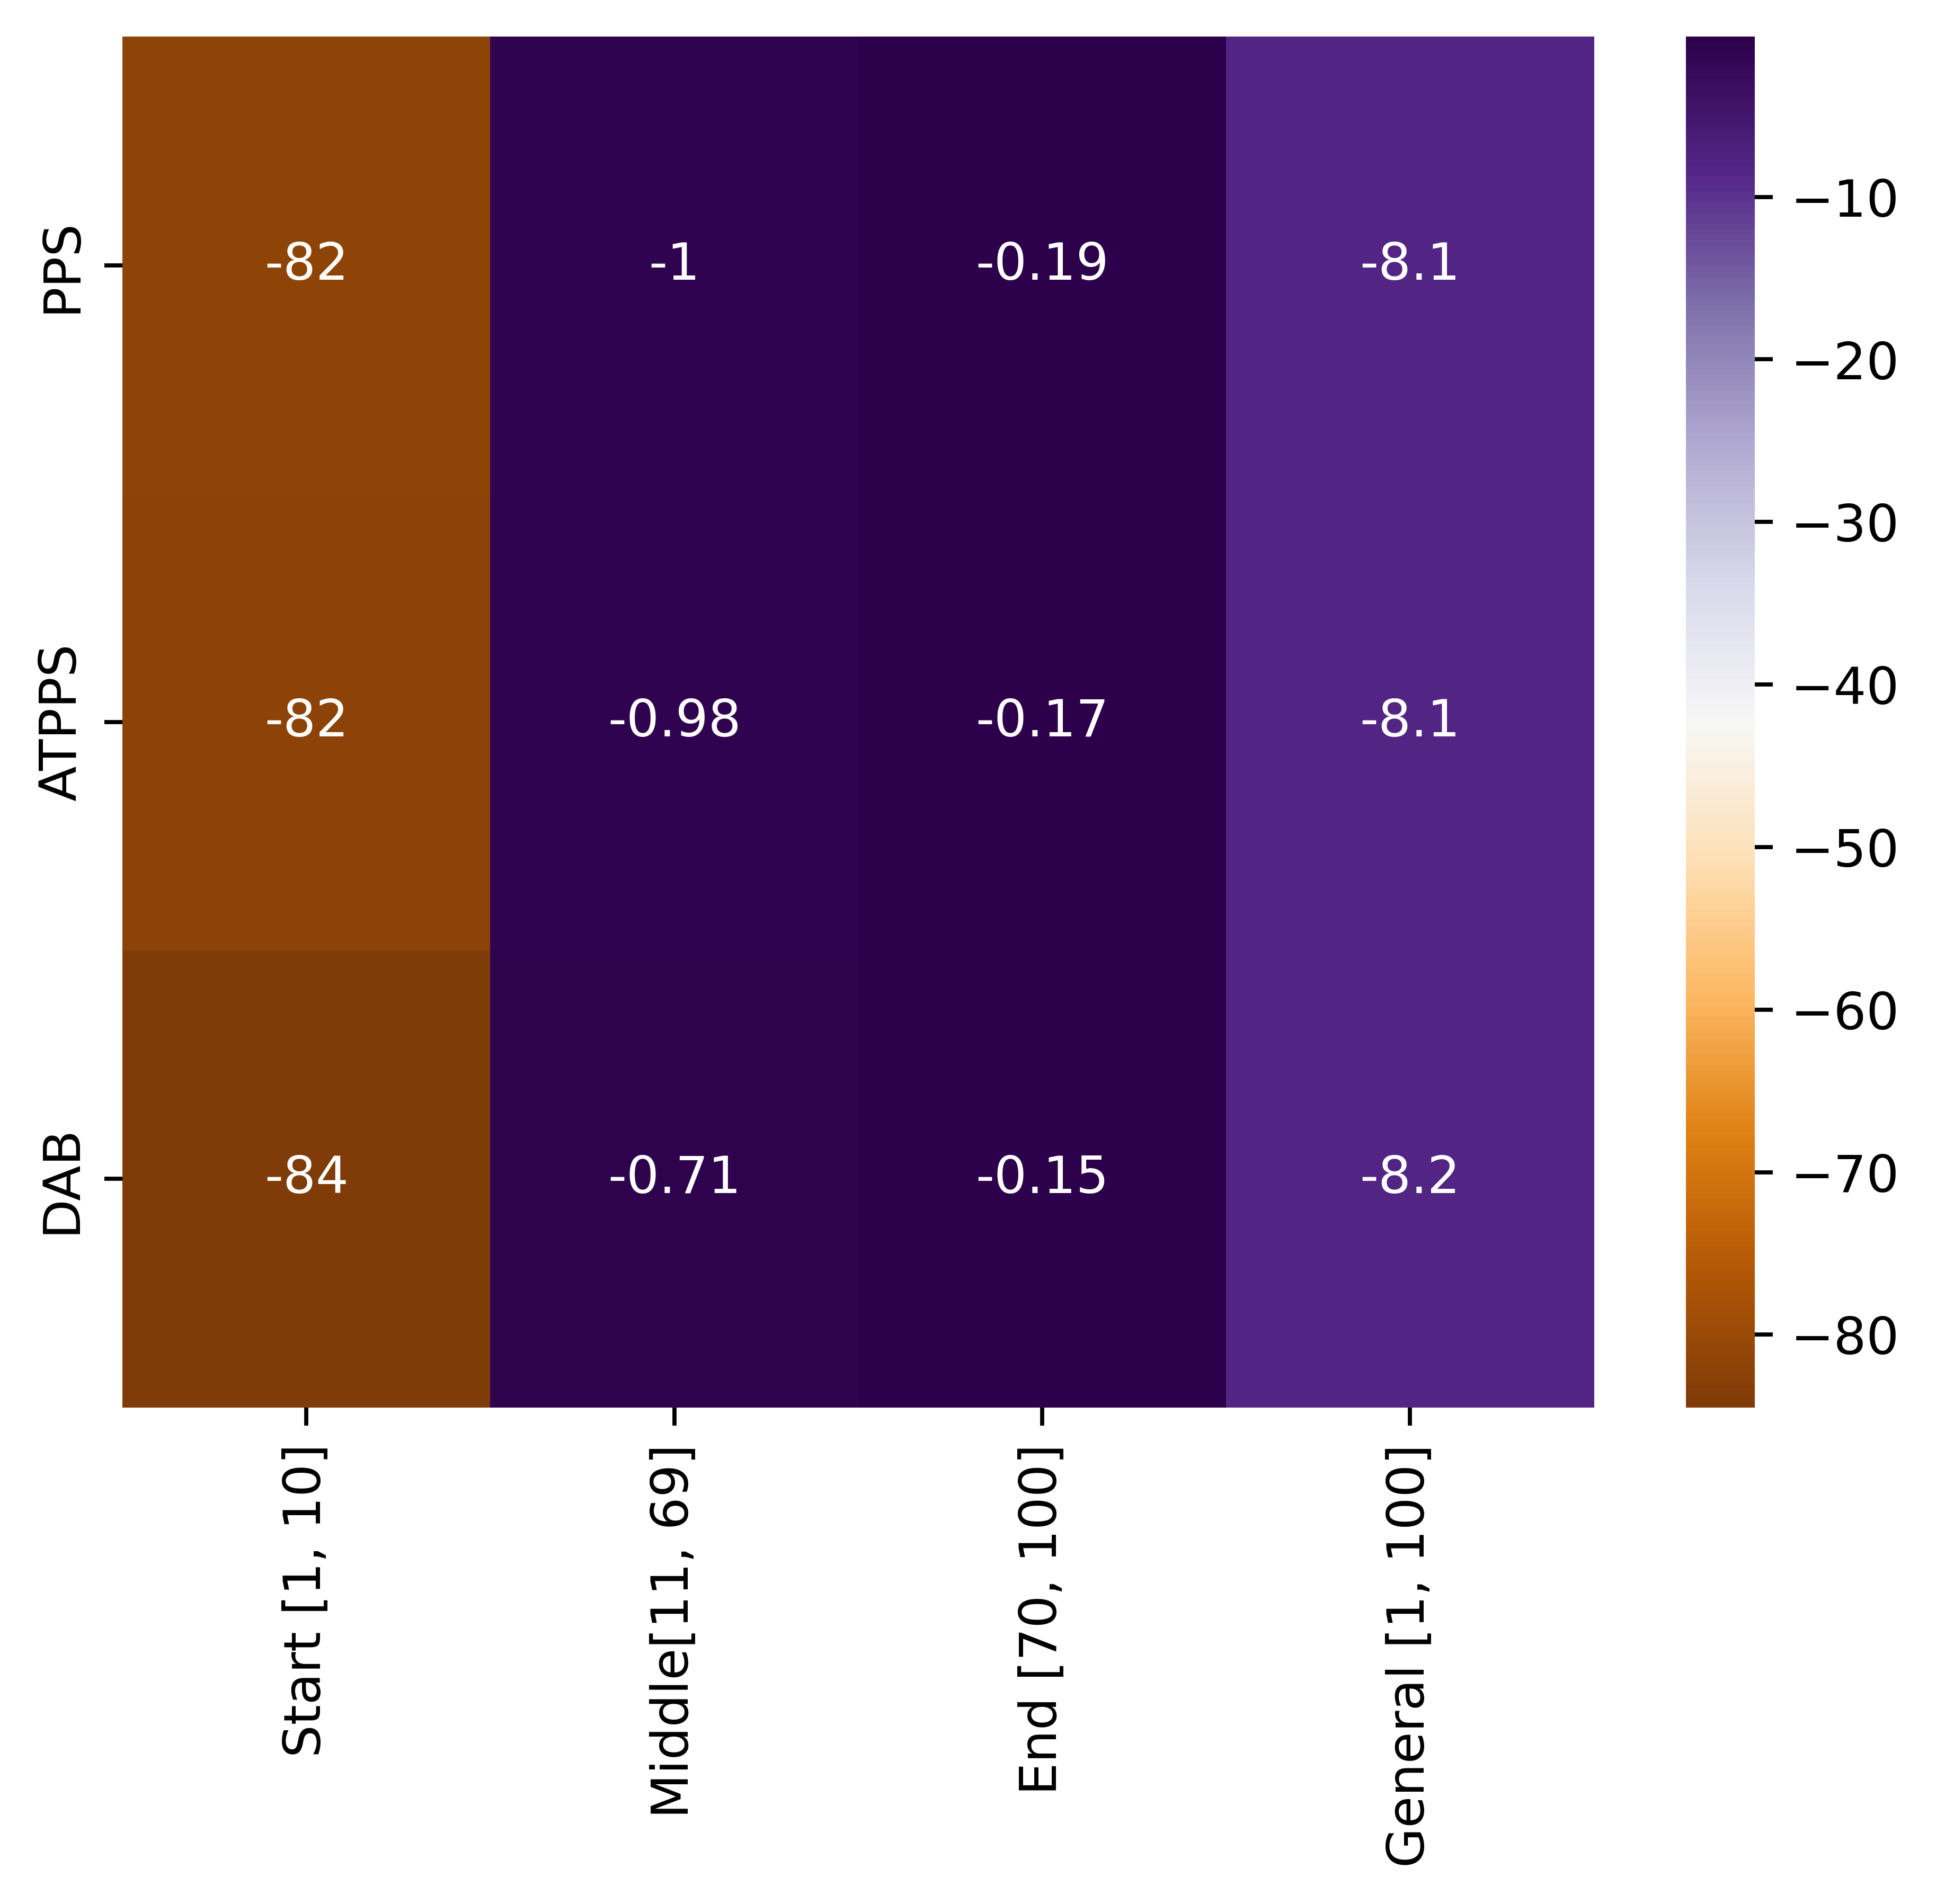
\includegraphics{figures/Simulation_outcomes/RingGraph/DAB_vs_PPS_vs_ATPPS_slopesheatmap_100rounds.png}}
%     \caption{Ring Graph: heat map of slopes per region}
%     \label{fig:ringgraphslopes}
% \end{figure}

\section{Torus Grid Graph}\label{sec:torusgridGraph}
Figure \ref{fig:torusMSEperRoundLogLog} shows the MSE reduction over rounds on a Torus Grid Graph, plotted on a log-log scale. At the beginning all three algorithms start with similar MSE values around 1000. The DAB algorithms curve appears to have a slightly slower initial reduction compared to PPS algorithms curve and ATPPS in the beginning (rounds 1 to 7). The slope in this region is superior for the DAB algorithm with a value of -140 compared to -130 for the PPS based algorithms (figure \ref{fig:torusgraphslopes}). PPS's curve and ATPPS's curve maintain nearly identical performances during the middle phase so the rounds 8 to 40, reducing MSE at a similar rate, with a slope of -1 for the PPS curve and -0.83 for the ATPPS curve. DAB shows a noticeable improvement over both PPS and ATPPS, achieving lower MSE values consistently. This suggests that DAB adapts more efficiently to the graph's structure during the intermediate (rounds in the middle) rounds. DAB continues to reduce MSE more effectively than the PPS-based protocols in the end region (rounds 41 to 100). PPS and ATPPS exhibit convergence, but they lag behind the DAB algorithm in reaching minimal MSE. A torus grid has more structured connectivity compared to a star or ring graph, allowing better distribution of loads via localized interactions. DAB's deterministic approach benefits from leveraging this regularity, leading to its superior performance.The ATPPS algorithm introduced in this paper achieves a compromise solution in this scenario. It seems to perform better than the classic PPS approach judging from the simulation outcomes, especially in later rounds, where the adaptiveness condition prevents "redundant" load transfers from happening and prioritizing load transfers that reduce the error impactful.

The uniform neighborhood structure of a torus ensures that DAB's deterministic decisions (e.g., always choosing the minimal neighbor) are consistently effective across the graph. The protocol doesn't suffer from random noise introduced by probabilistic neighbor choices, making it inherently well-suited to the topology. Both PPS and ATPPS protocols rely on randomly selecting a neighbor for load exchange. While this randomness is beneficial in irregular or dense graphs (e.g., star or complete graphs), it is less effective in structured topologies compared to the DAB like a torus. The PPS-based algorithms do not always target the most unbalanced areas. This means that load propagation can sometimes "stall" in certain regions, requiring more rounds to achieve global balance.

The fitted polynomial curve of degree 5 matches the MSE data for DAB effectively, capturing the nonlinear dynamics during rounds 10 to 39 following the equation: $MSE_r=-1.35*10^{-6} + 1.89*10^{-4}r-0.01r^{2}+0.30r^{3}-4.6r^{4}+34.10r^{5}$. This suggests that in the early rounds (10 to 39), the MSE reduction follows a complex pattern due to the DAB's optimization mechanism, such as its focus on minimizing neighbors loads dynamically. The higher degree captures these dynamics with more precision than simpler models. In later rounds the performance of the DAB can still be captured by a polynomial curve with equation: $MSE_r=-6.01*10^{-06}+1.66*10^{-3}r-0.16r^{2}+6r^{3}$. The fitted polynomial curve of degree 4 fits the MSE data well in later rounds. By this stage, the load balancing has stabilized, and the reduction in MSE is more linear or gradual. A lower-degree polynomial suffices for rounds 40 to 100 since the dynamics are simpler compared to the earlier rounds. The curve behaviour for the PPS and ATPPS are similar to that of the DAB curve expressed for rounds 10 to 40 by the equations: $MSE_r=-5.54*10^{-06}+7.65*10^{-4}r-0.04r^{2}+1.16r^{3}-16.81r^{4}+112.86r^{5}$ for the PPS and: $MSE_r = -3.65 \times 10^{-6} + 5.16 \times 10^{-4}r - 0.03r^{2} + 0.83r^{3} - 12.52r^{4} + 88.16r^{5}$ for the ATPPS. The $r^{5}$ term ($88.16*r^{5}$) dominates the polynomial at higher rounds. This reflects the initial high variance (high MSE) at the start of the process when nodes have not yet balanced their loads effectively.As rounds progress, the lower-degree terms (e.g., $r^{4}$ and $r^{3}$) become more influential. These represent the gradual stabilization of the MSE as the load balances across the graph. The negative coefficients for $r^{4}$ ($-12.52r^{4}$) and lower powers ($-0.03r^{2}$) show the decline of MSE over time as the algorithm pushes load differences to zero. The values slightly differ for the other algorithms but the idea is the same, as the fitted models for each algorithm are structured the same. The equations that describe that are fitted to the MSE data for the rounds for the rounds 41 to 100 for the PPS is:$MSE_r = -1.15 \times 10^{-5} + 3.205\times 10^{-3}r - 0.33r^2 + 13.72r^3$ and for the ATPPS is: $MSE_r = -9.99 \times 10^{-6} + 2.8034\times 10^{-3}r - 0.28r^2 + 11.29r^3$. Here the structure is also similar, however described with less terms (degree 3).

% \begin{figure}[h]
%     \centering
%     \scalebox{0.5}{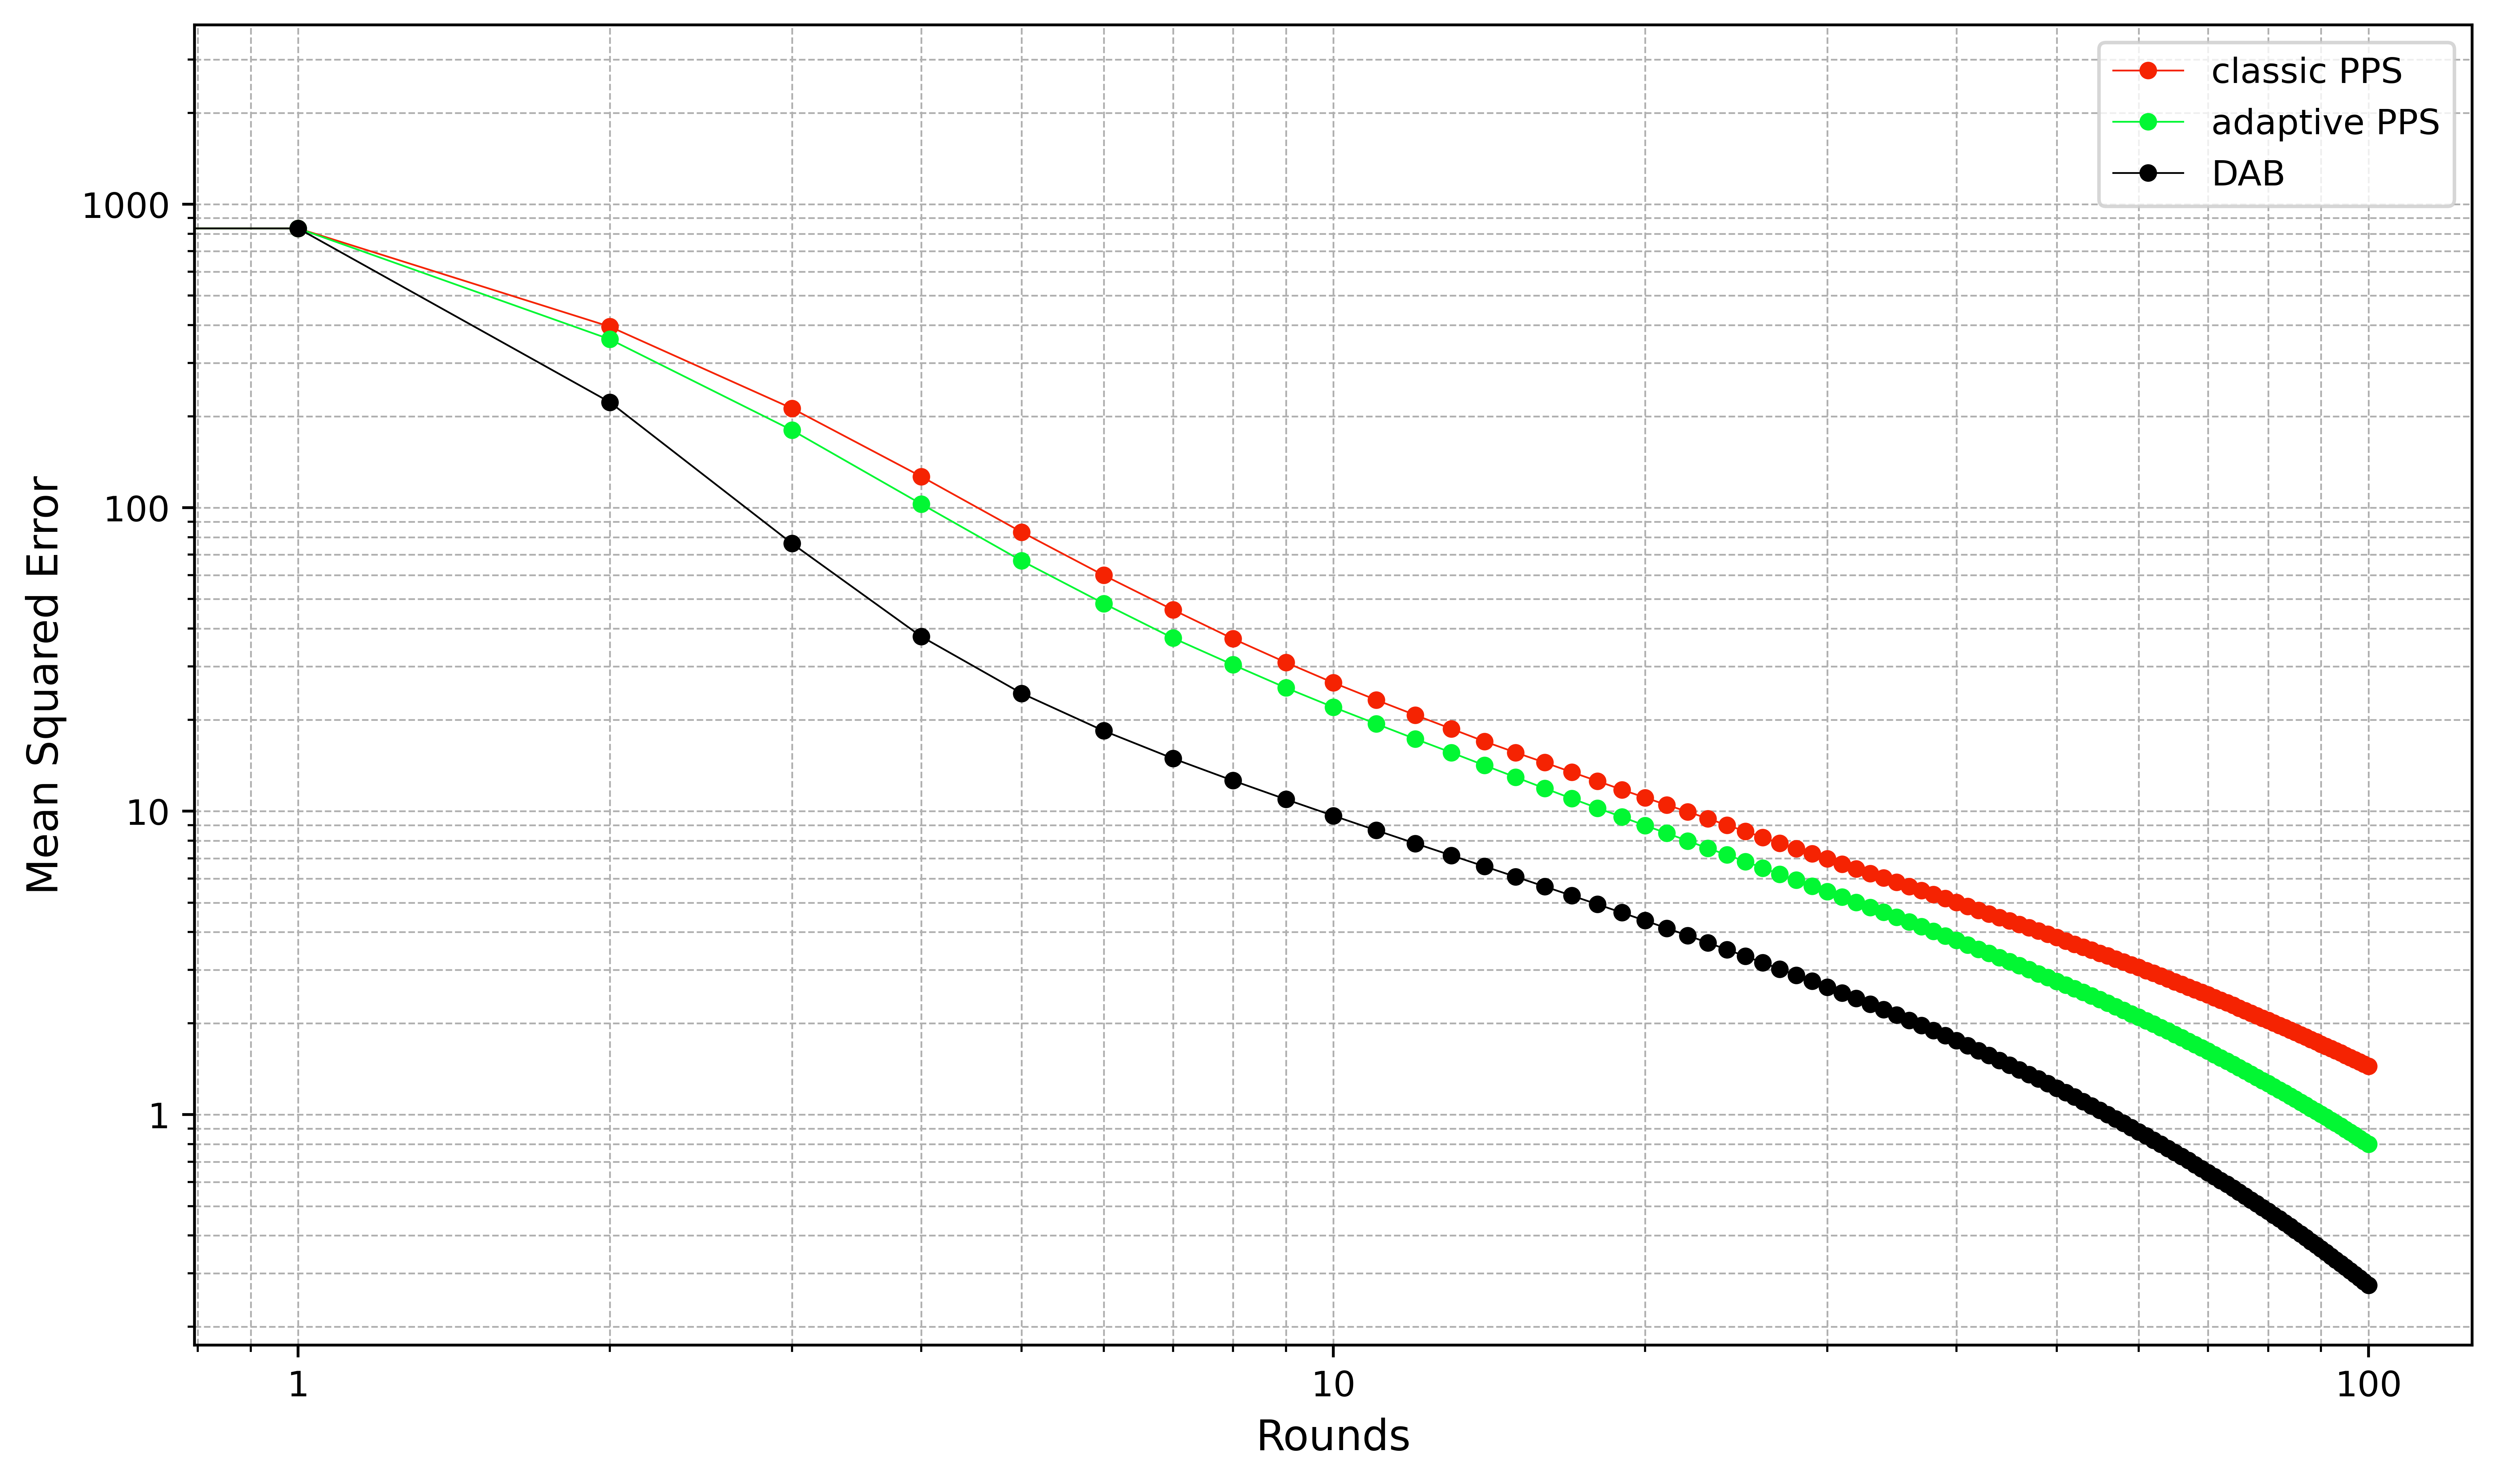
\includegraphics{figures/Simulation_outcomes/TorusGridGraph/DAB_vs_PPS_TGG_r100_n1024_averaged_loglog.png}}
%     \caption{Torus Grid Graph: mean squared error per rounds (log-log)}
%     \label{fig:torusMSEperRoundLogLog}
% \end{figure}

% \begin{figure}[!ht]
%     \centering
%         \subfloat[]{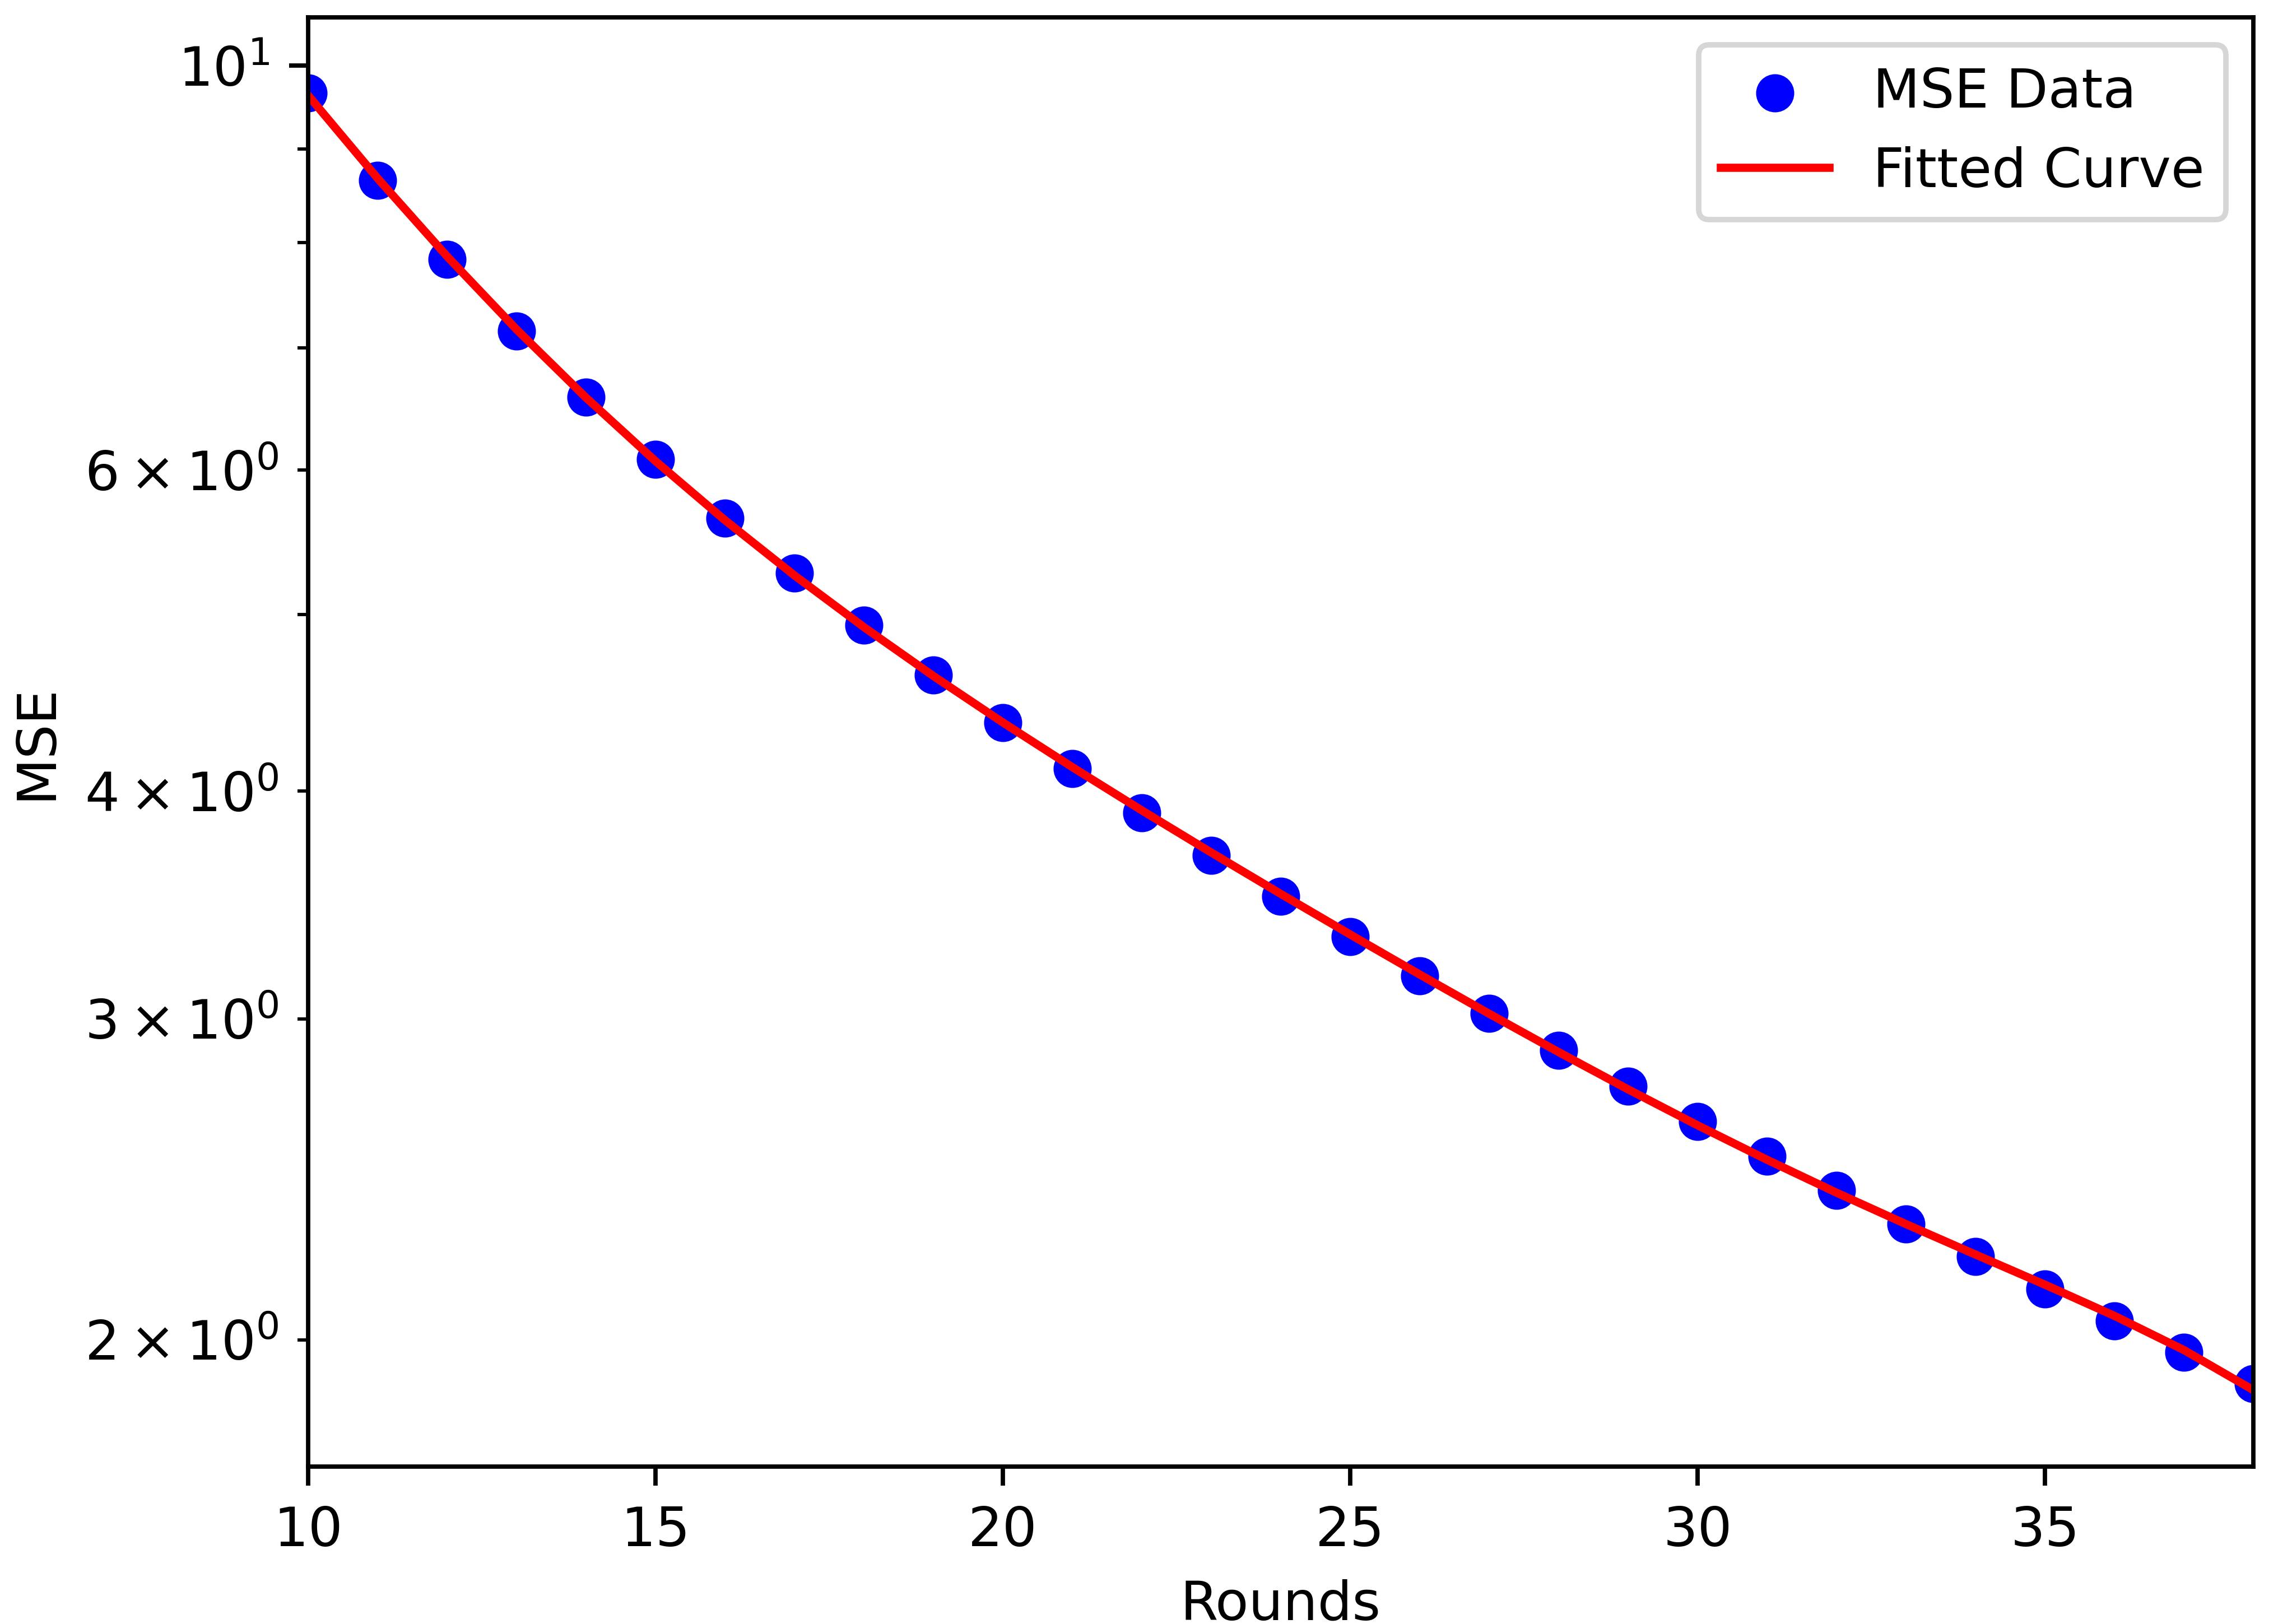
\includegraphics[width=0.49\linewidth]{figures/Simulation_outcomes/TorusGridGraph/DAB/DAB_modelfitting_rounds_38_model_2.png}}
%     \hfil
%         \subfloat[]{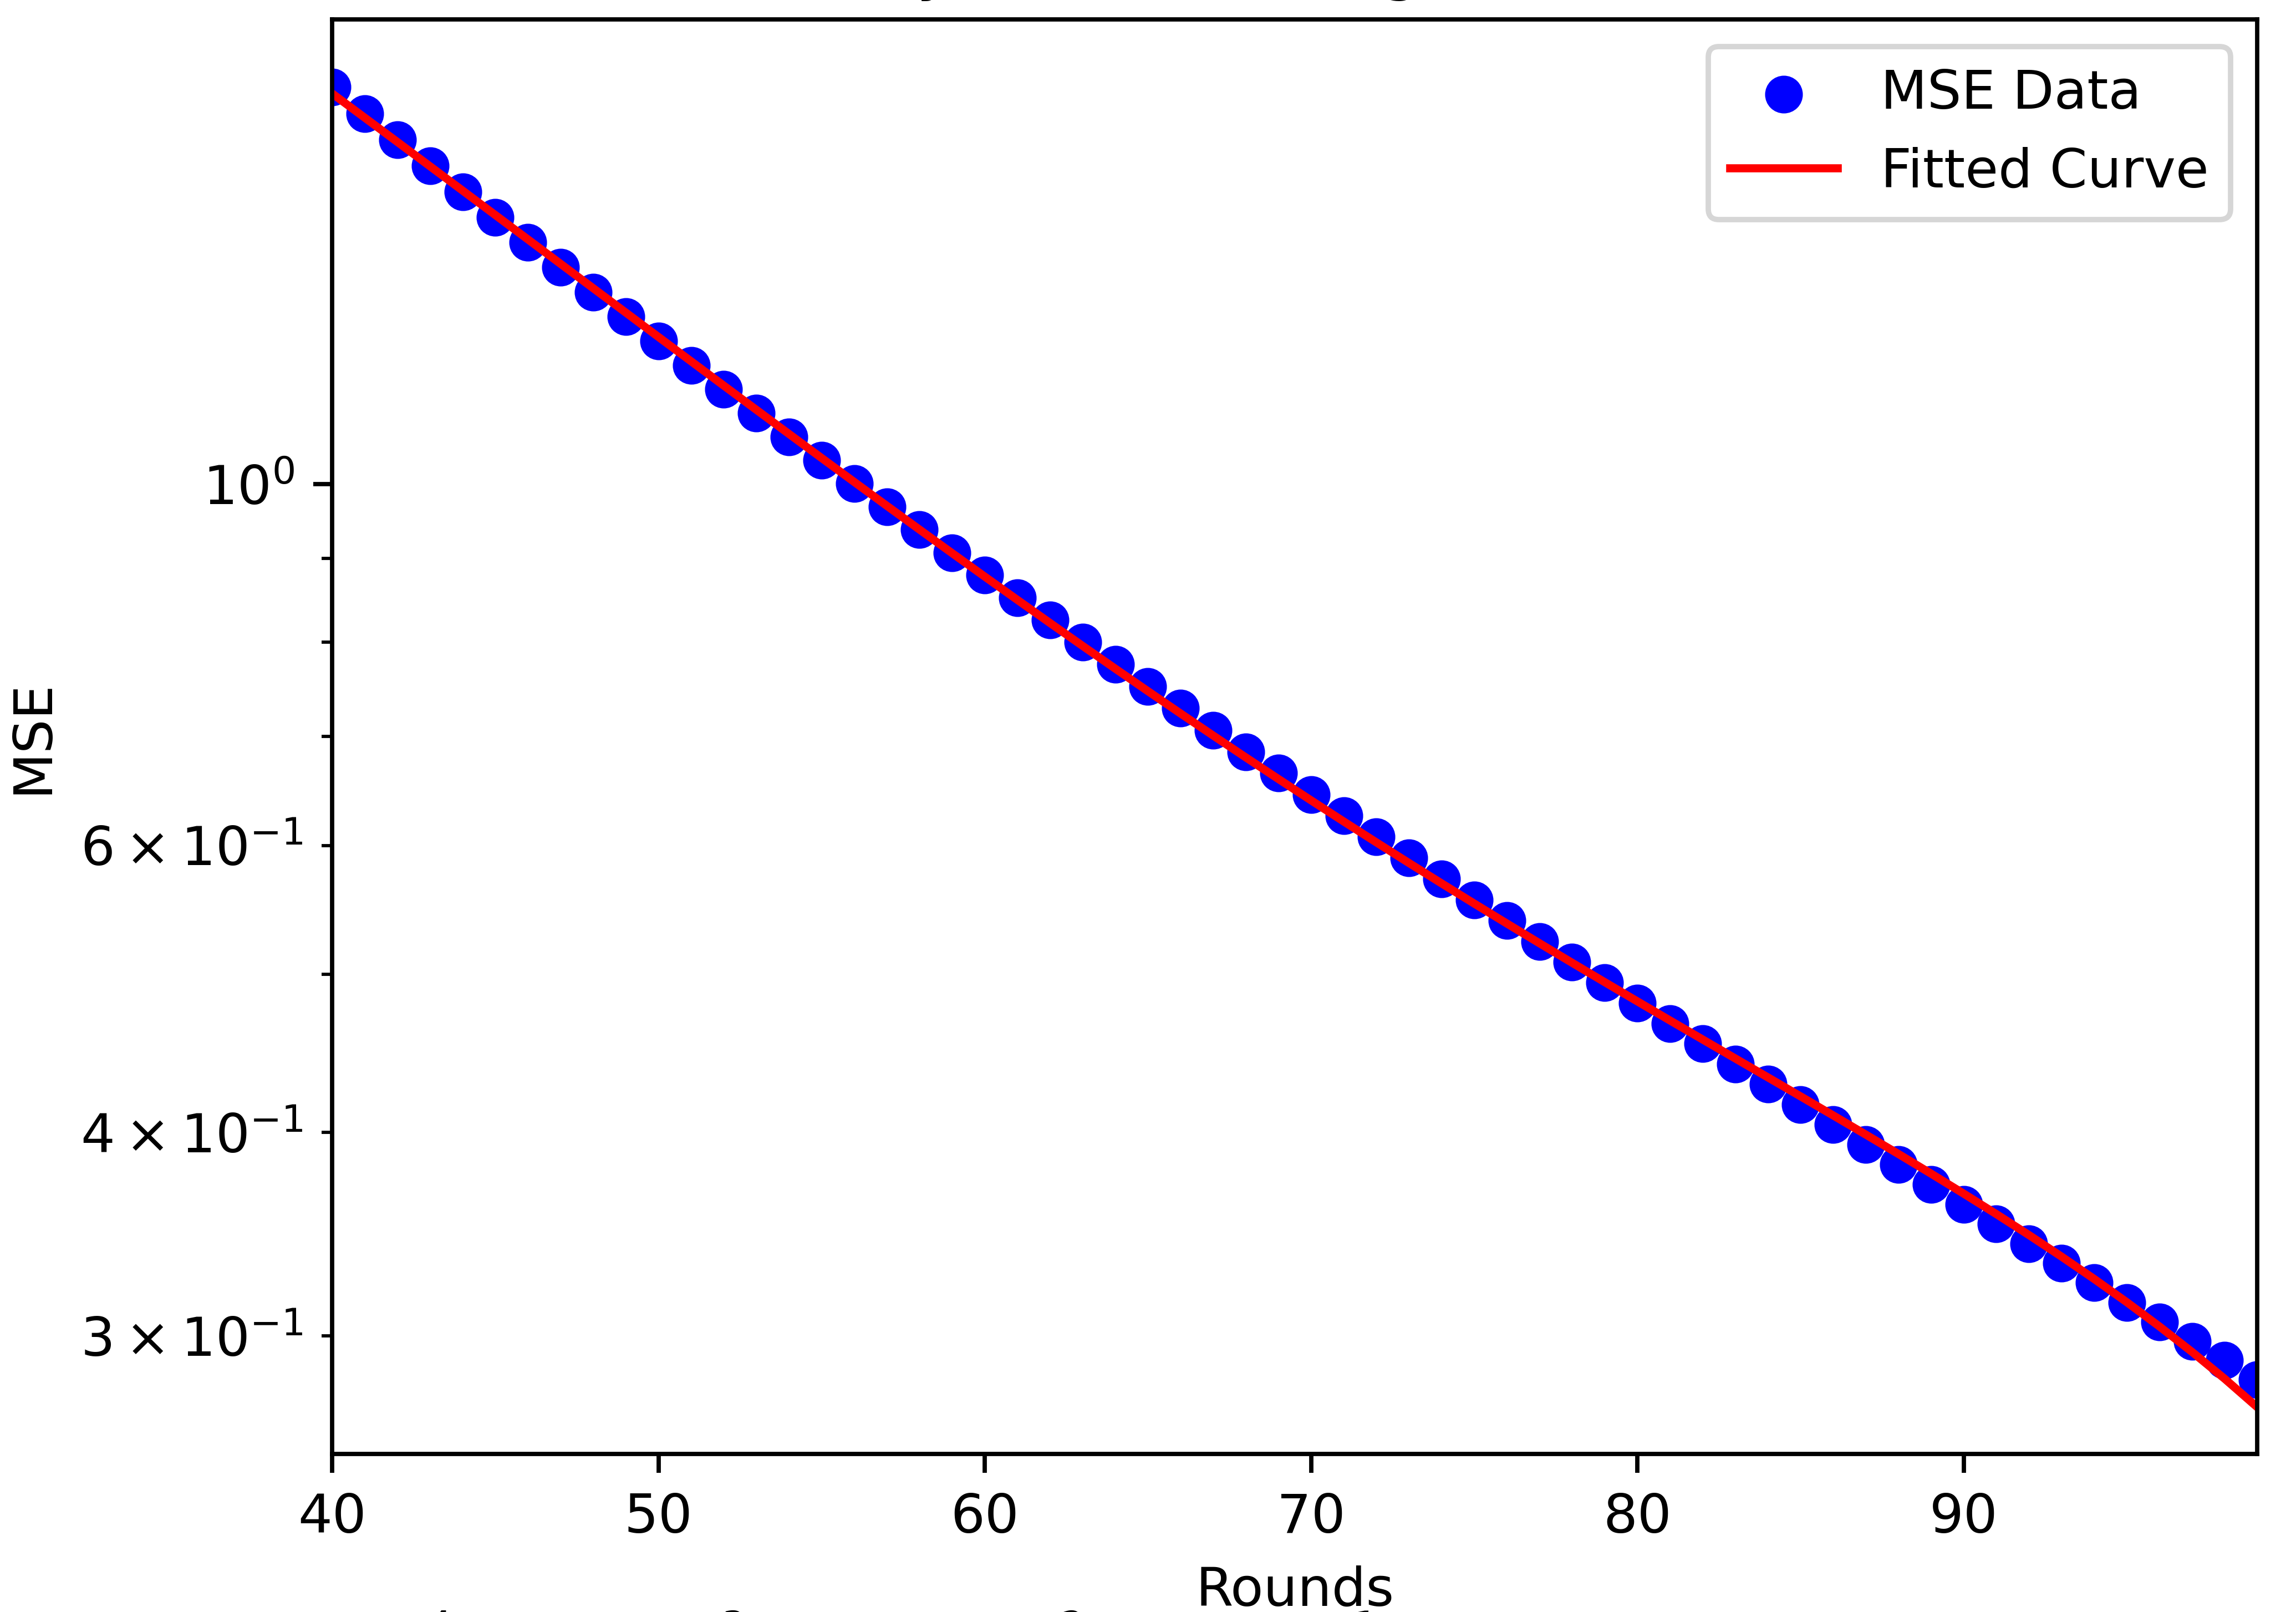
\includegraphics[width=0.49\linewidth]{figures/Simulation_outcomes/TorusGridGraph/DAB/DAB_modelfitting_rounds_99_model_2.png}}
%     \caption{Polynomial Regression Fit: DAB; Rounds 10-39 and 40-100}
%         \label{fig:dabTorusModelFit}
% \end{figure}

% \begin{figure}[!ht]
%     \centering
%         \subfloat[]{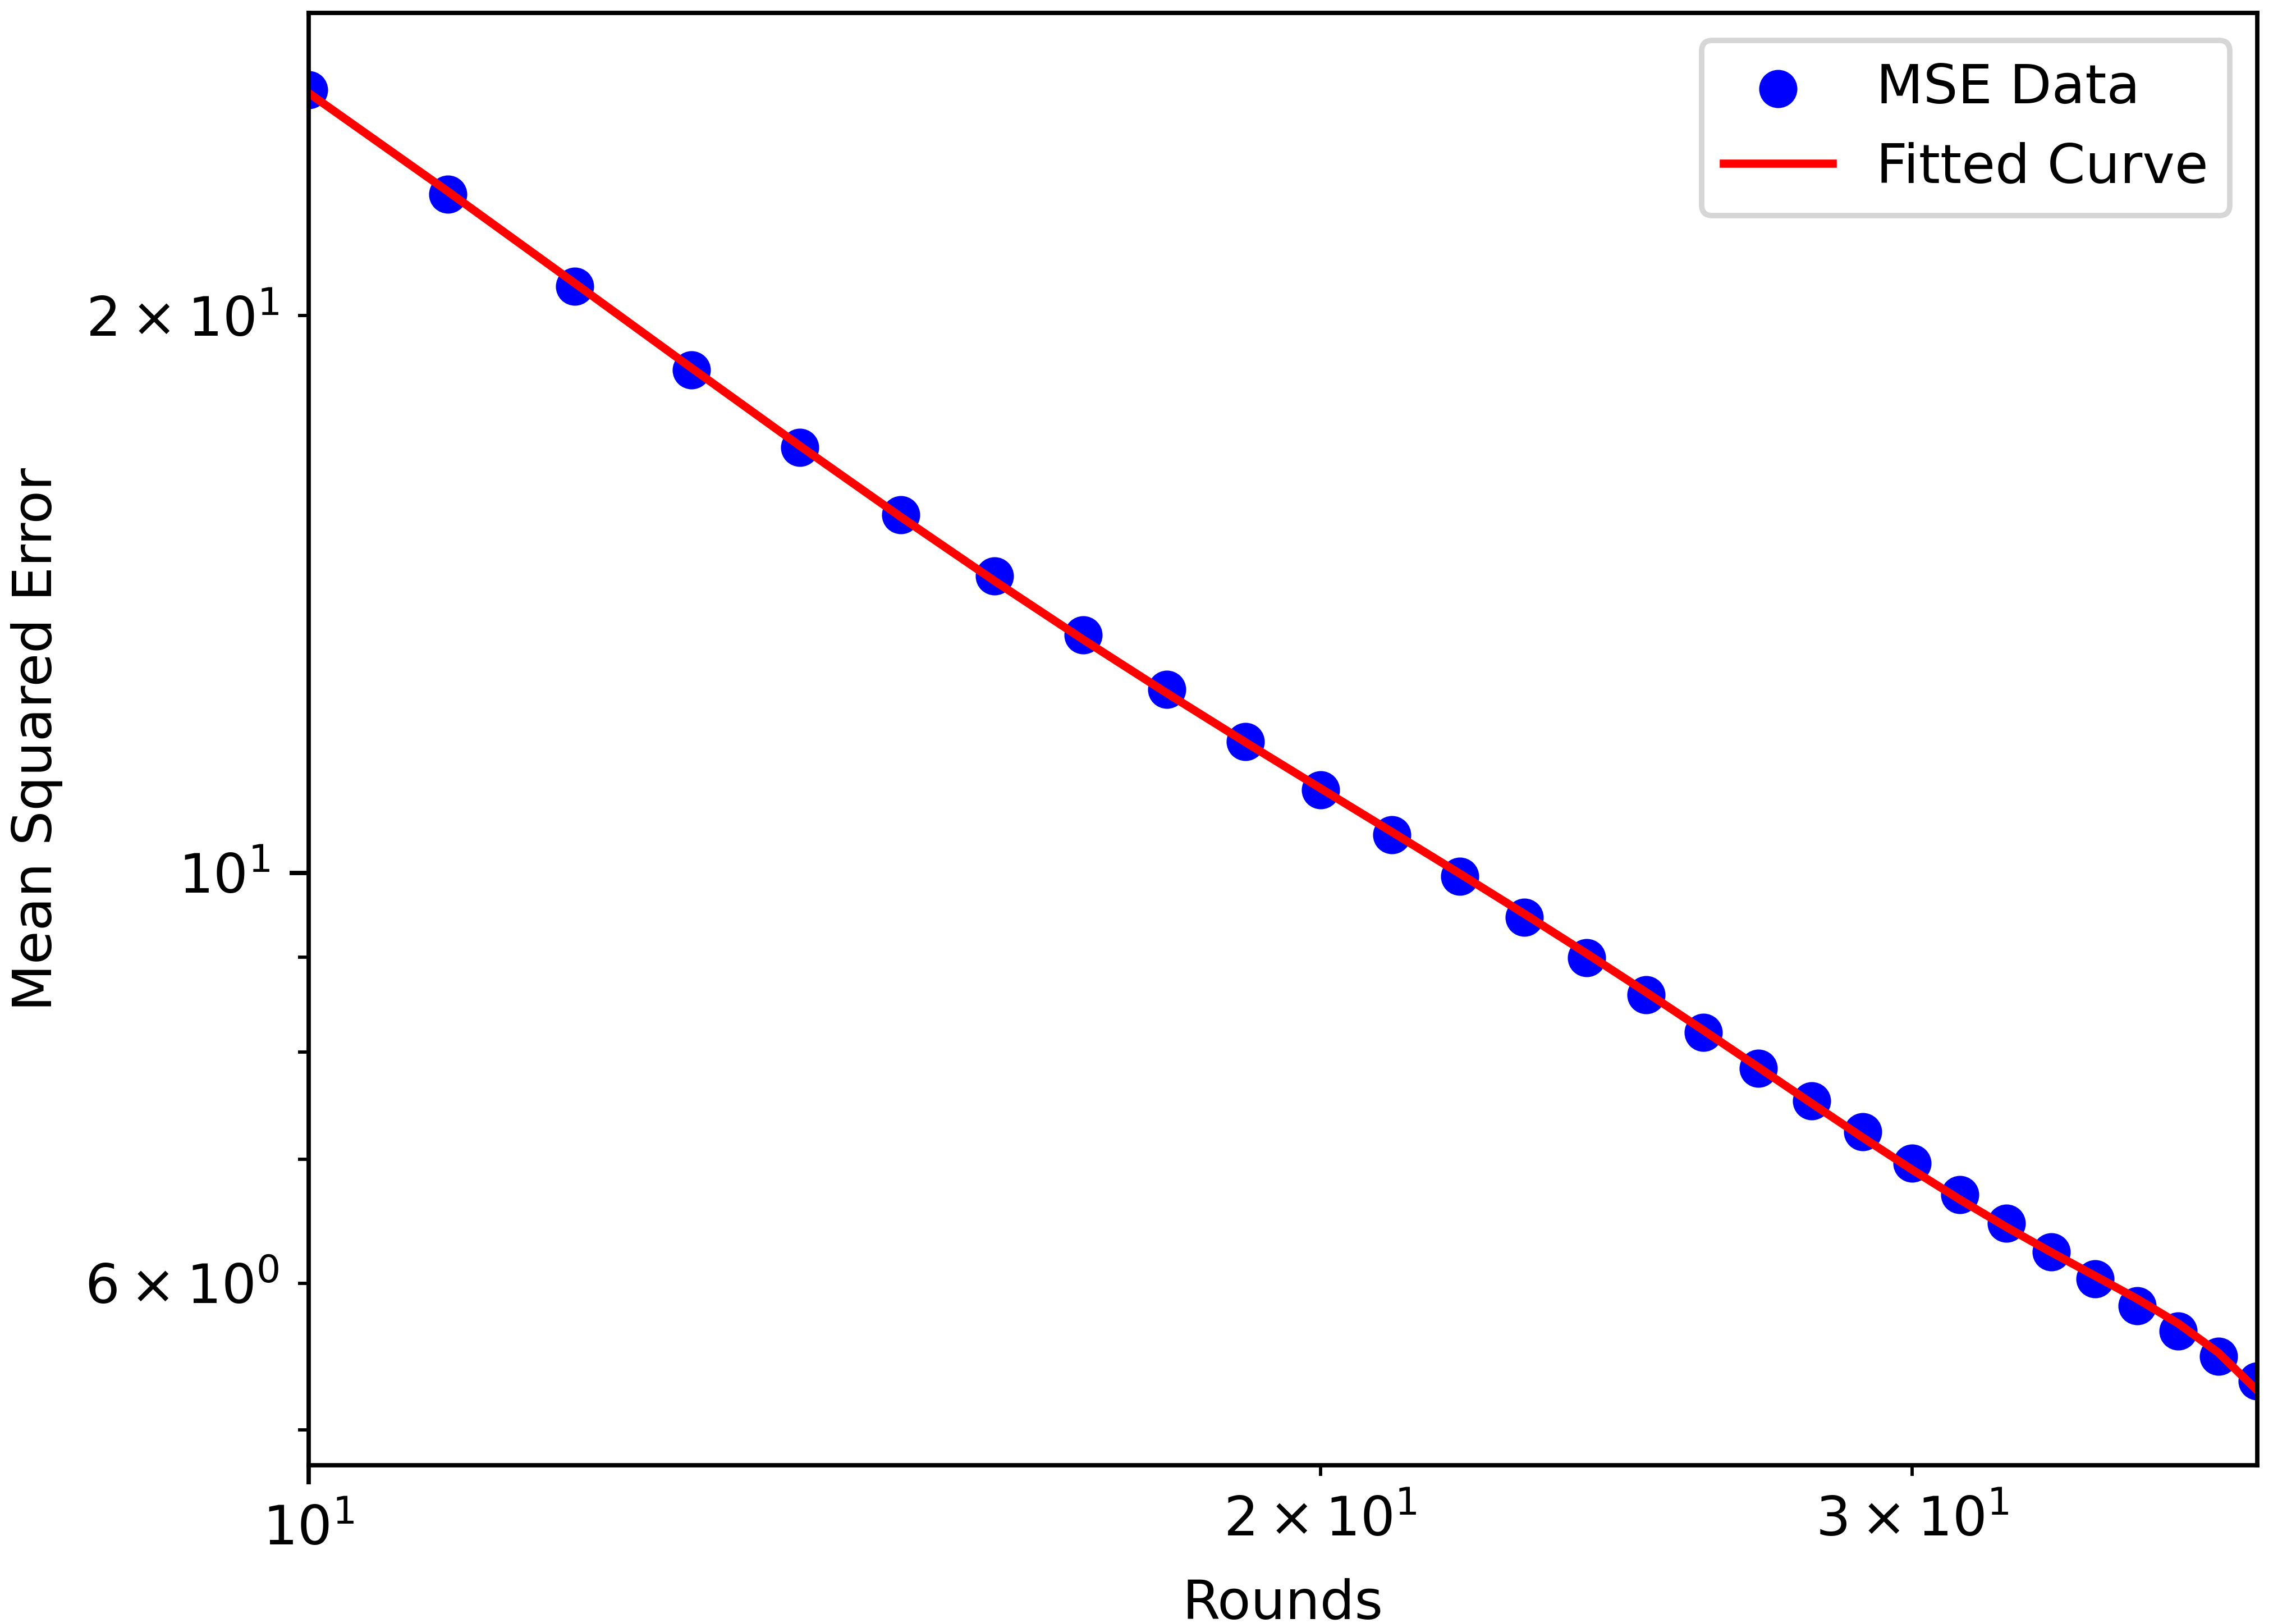
\includegraphics[width=0.49\linewidth]{figures/Simulation_outcomes/TorusGridGraph/PPS/PPS_modelfitting_rounds_38_model_2.png}}
%     \hfil
%         \subfloat[]{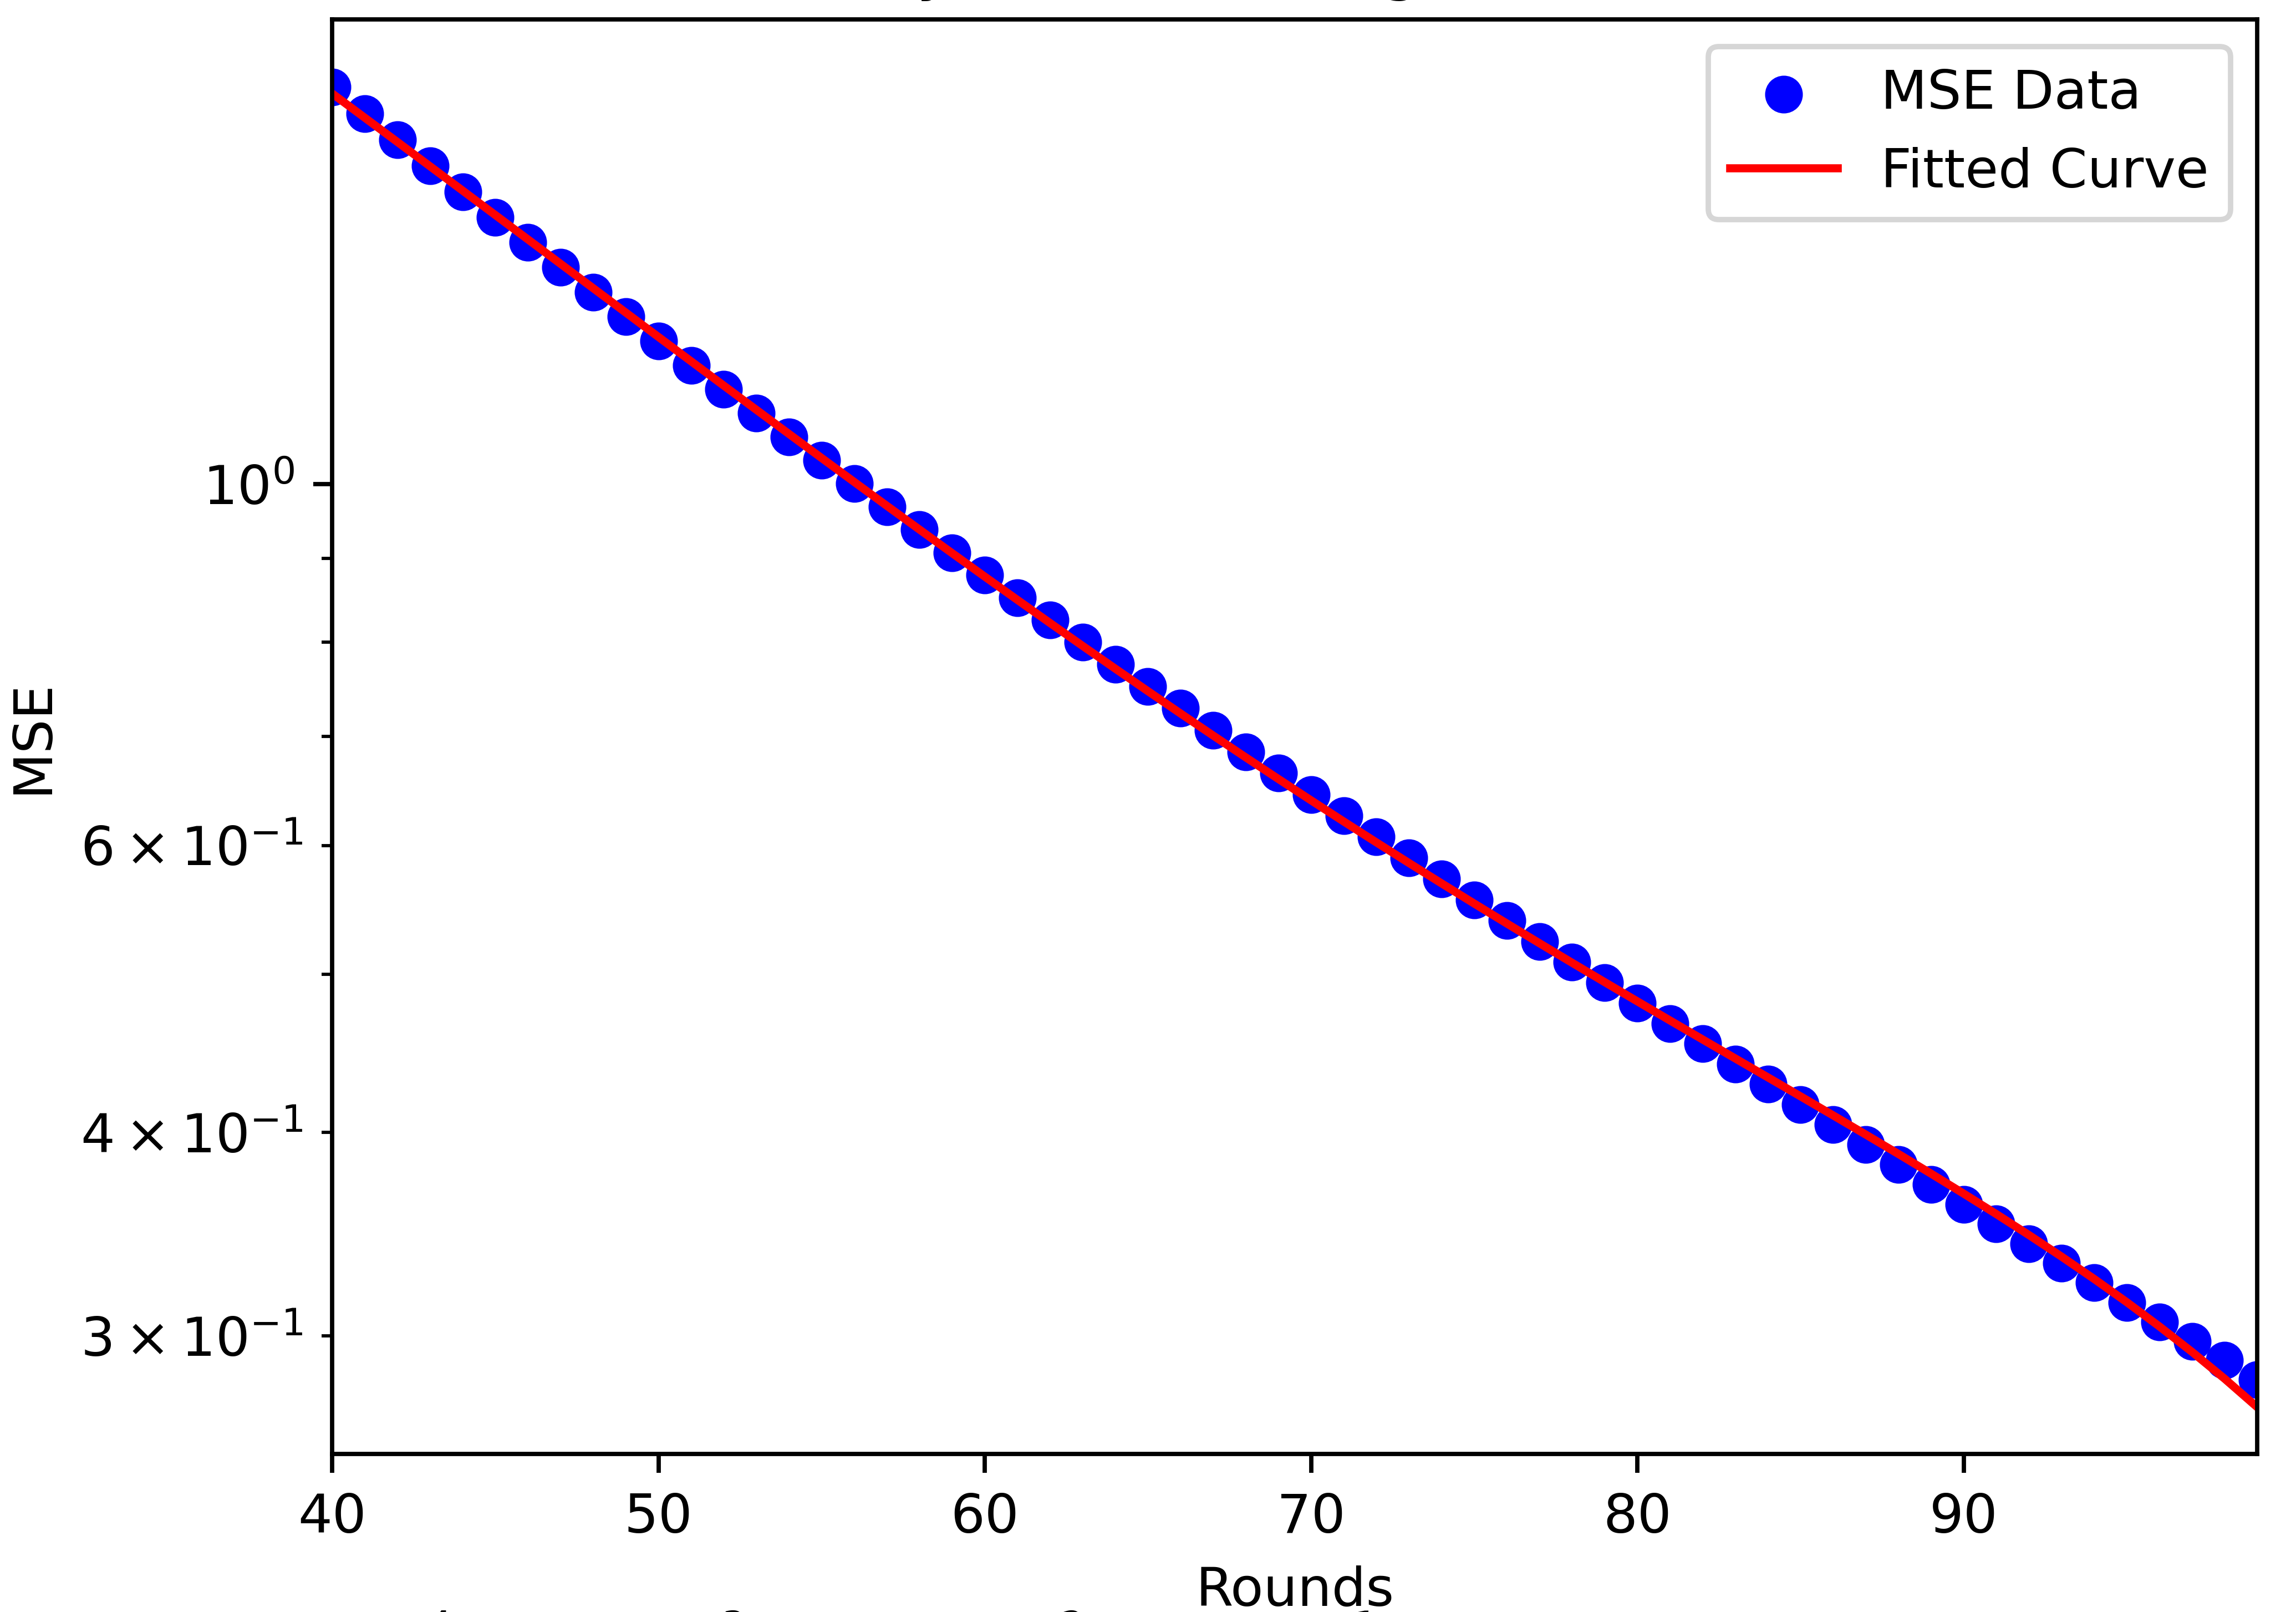
\includegraphics[width=0.49\linewidth]{figures/Simulation_outcomes/TorusGridGraph/DAB/DAB_modelfitting_rounds_99_model_2.png}}
%     \caption{Polynomial Regression Fit: PPS; Rounds 10-39 and 40-100}
%         \label{fig:ppsTorusModelFit}
% \end{figure}

%\begin{figure}[!ht]
%    \centering
%        \subfloat[]{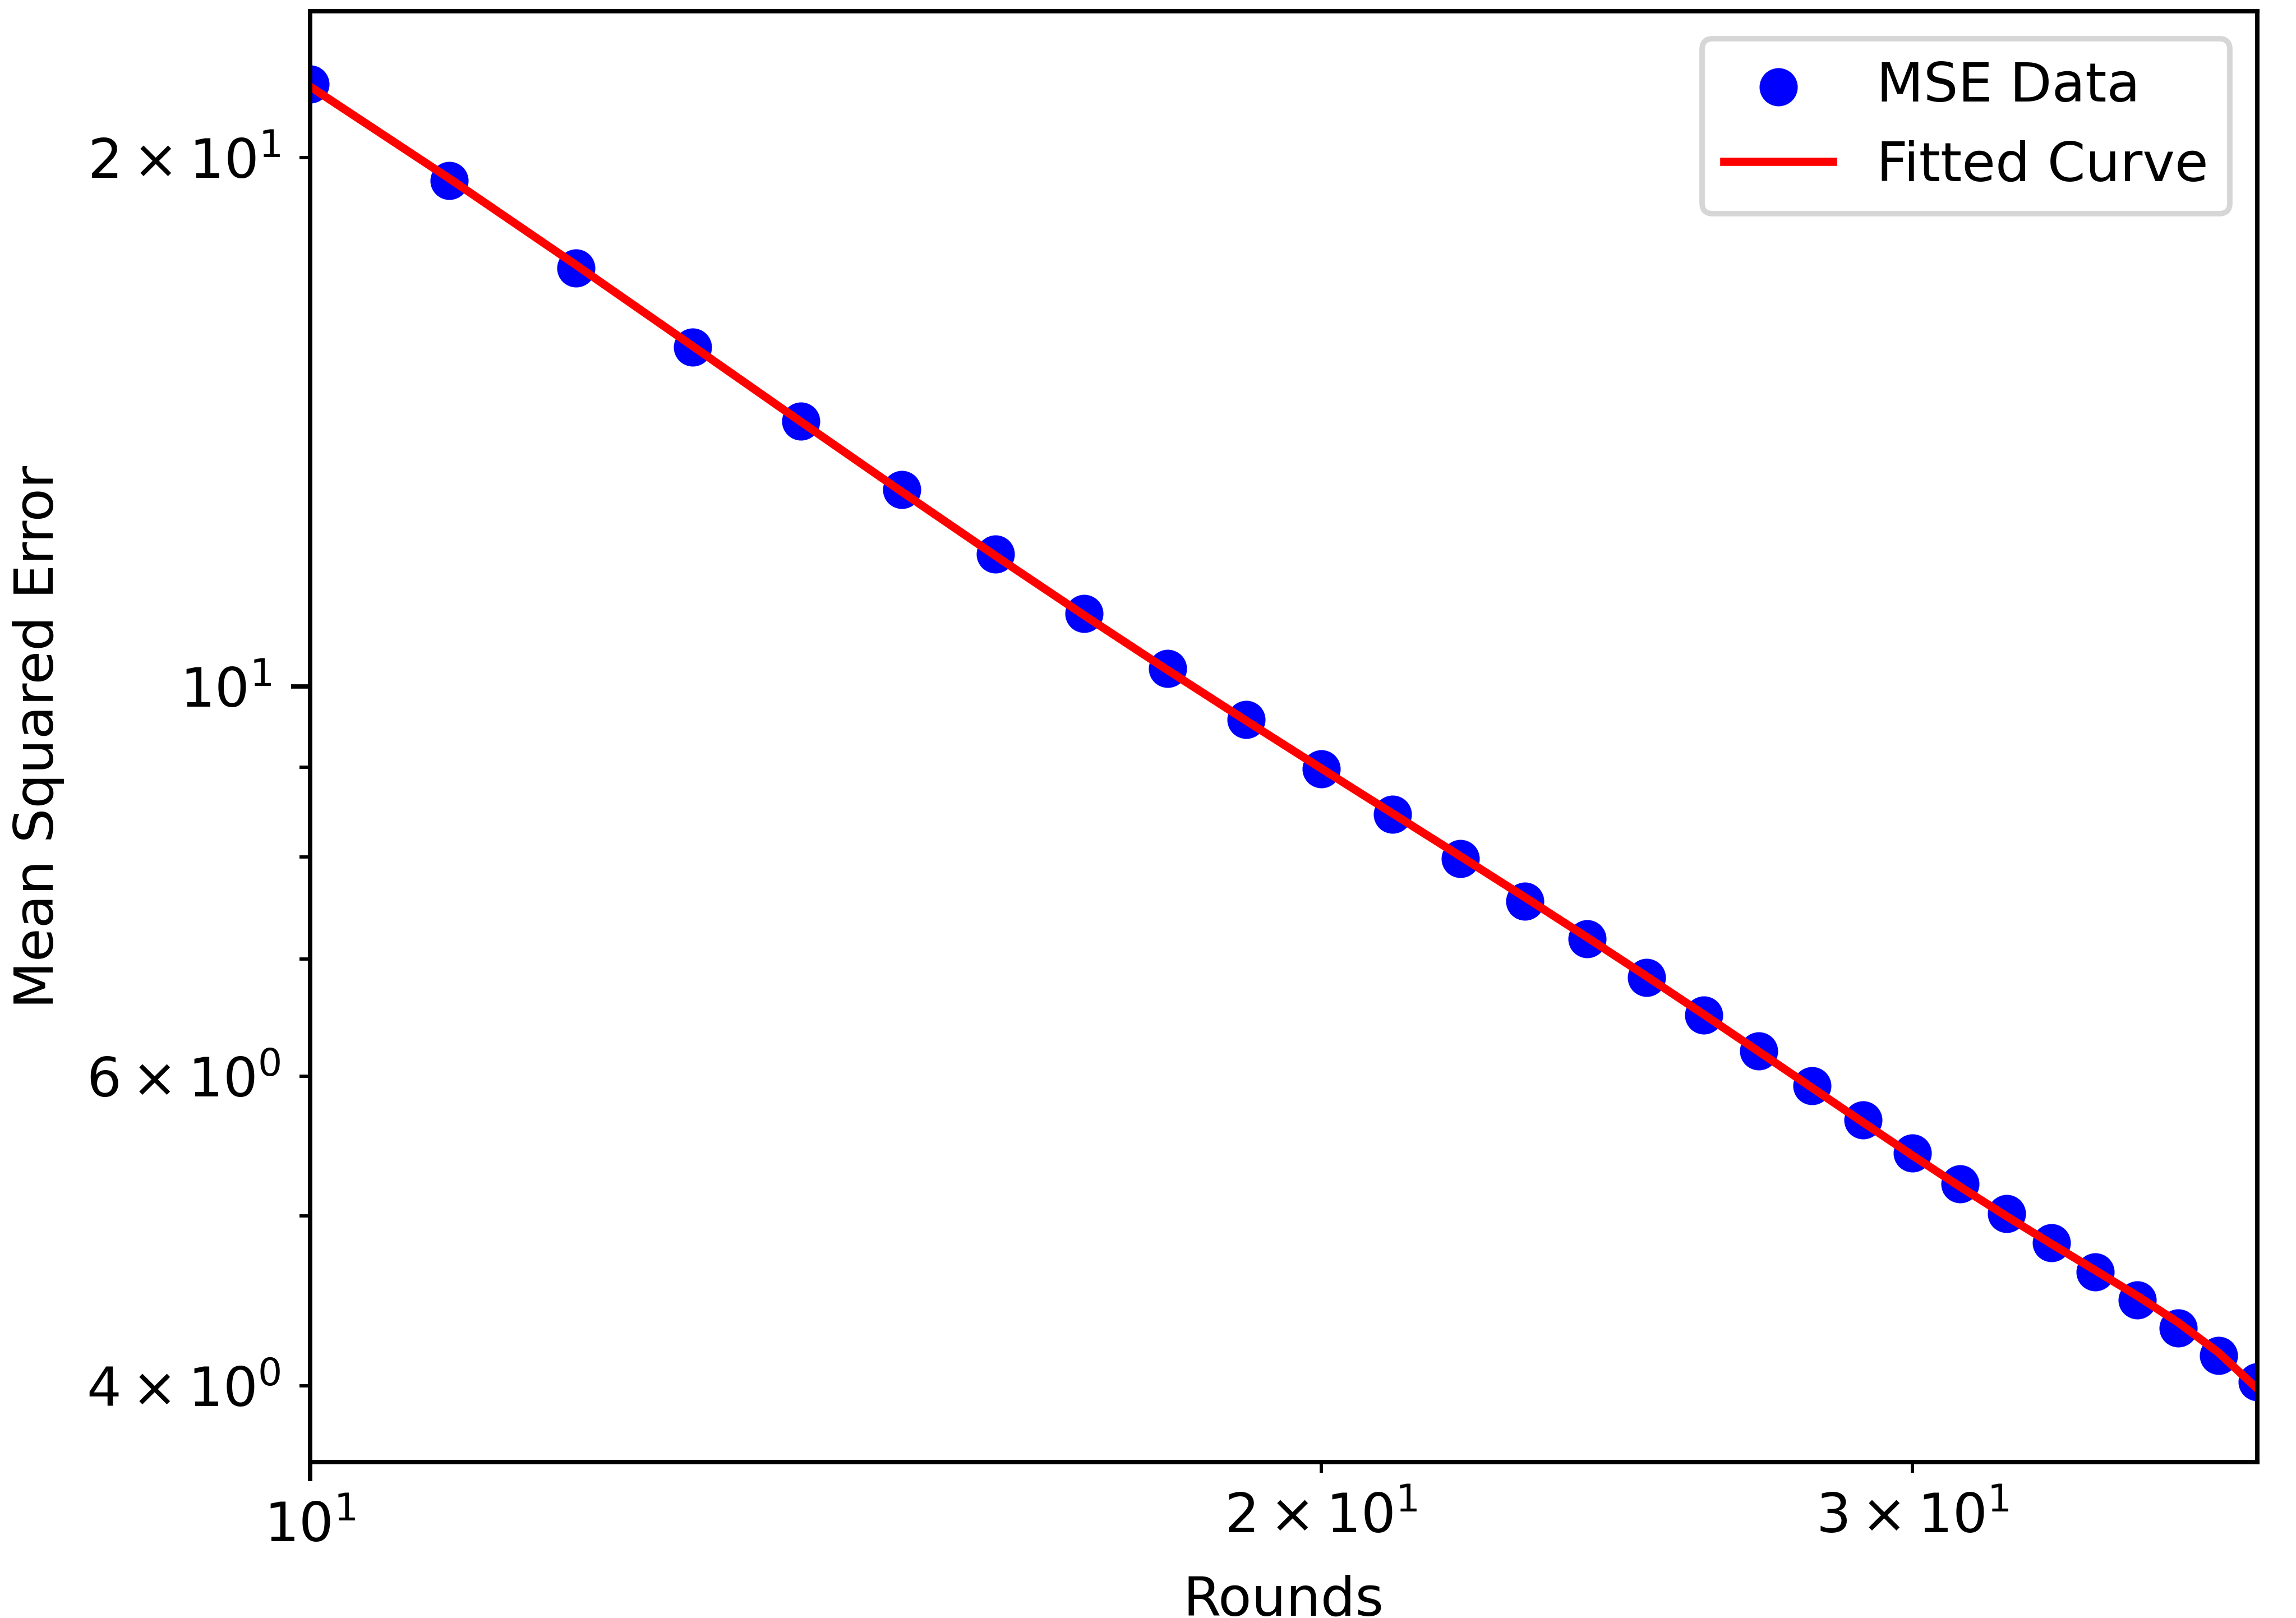
\includegraphics[width=0.49\linewidth]{figures/Simulation_outcomes/TorusGridGraph/ATPPS/ATPPS_modelfitting_rounds_38_model_2.png}}
%    \hfil
%        \subfloat[]{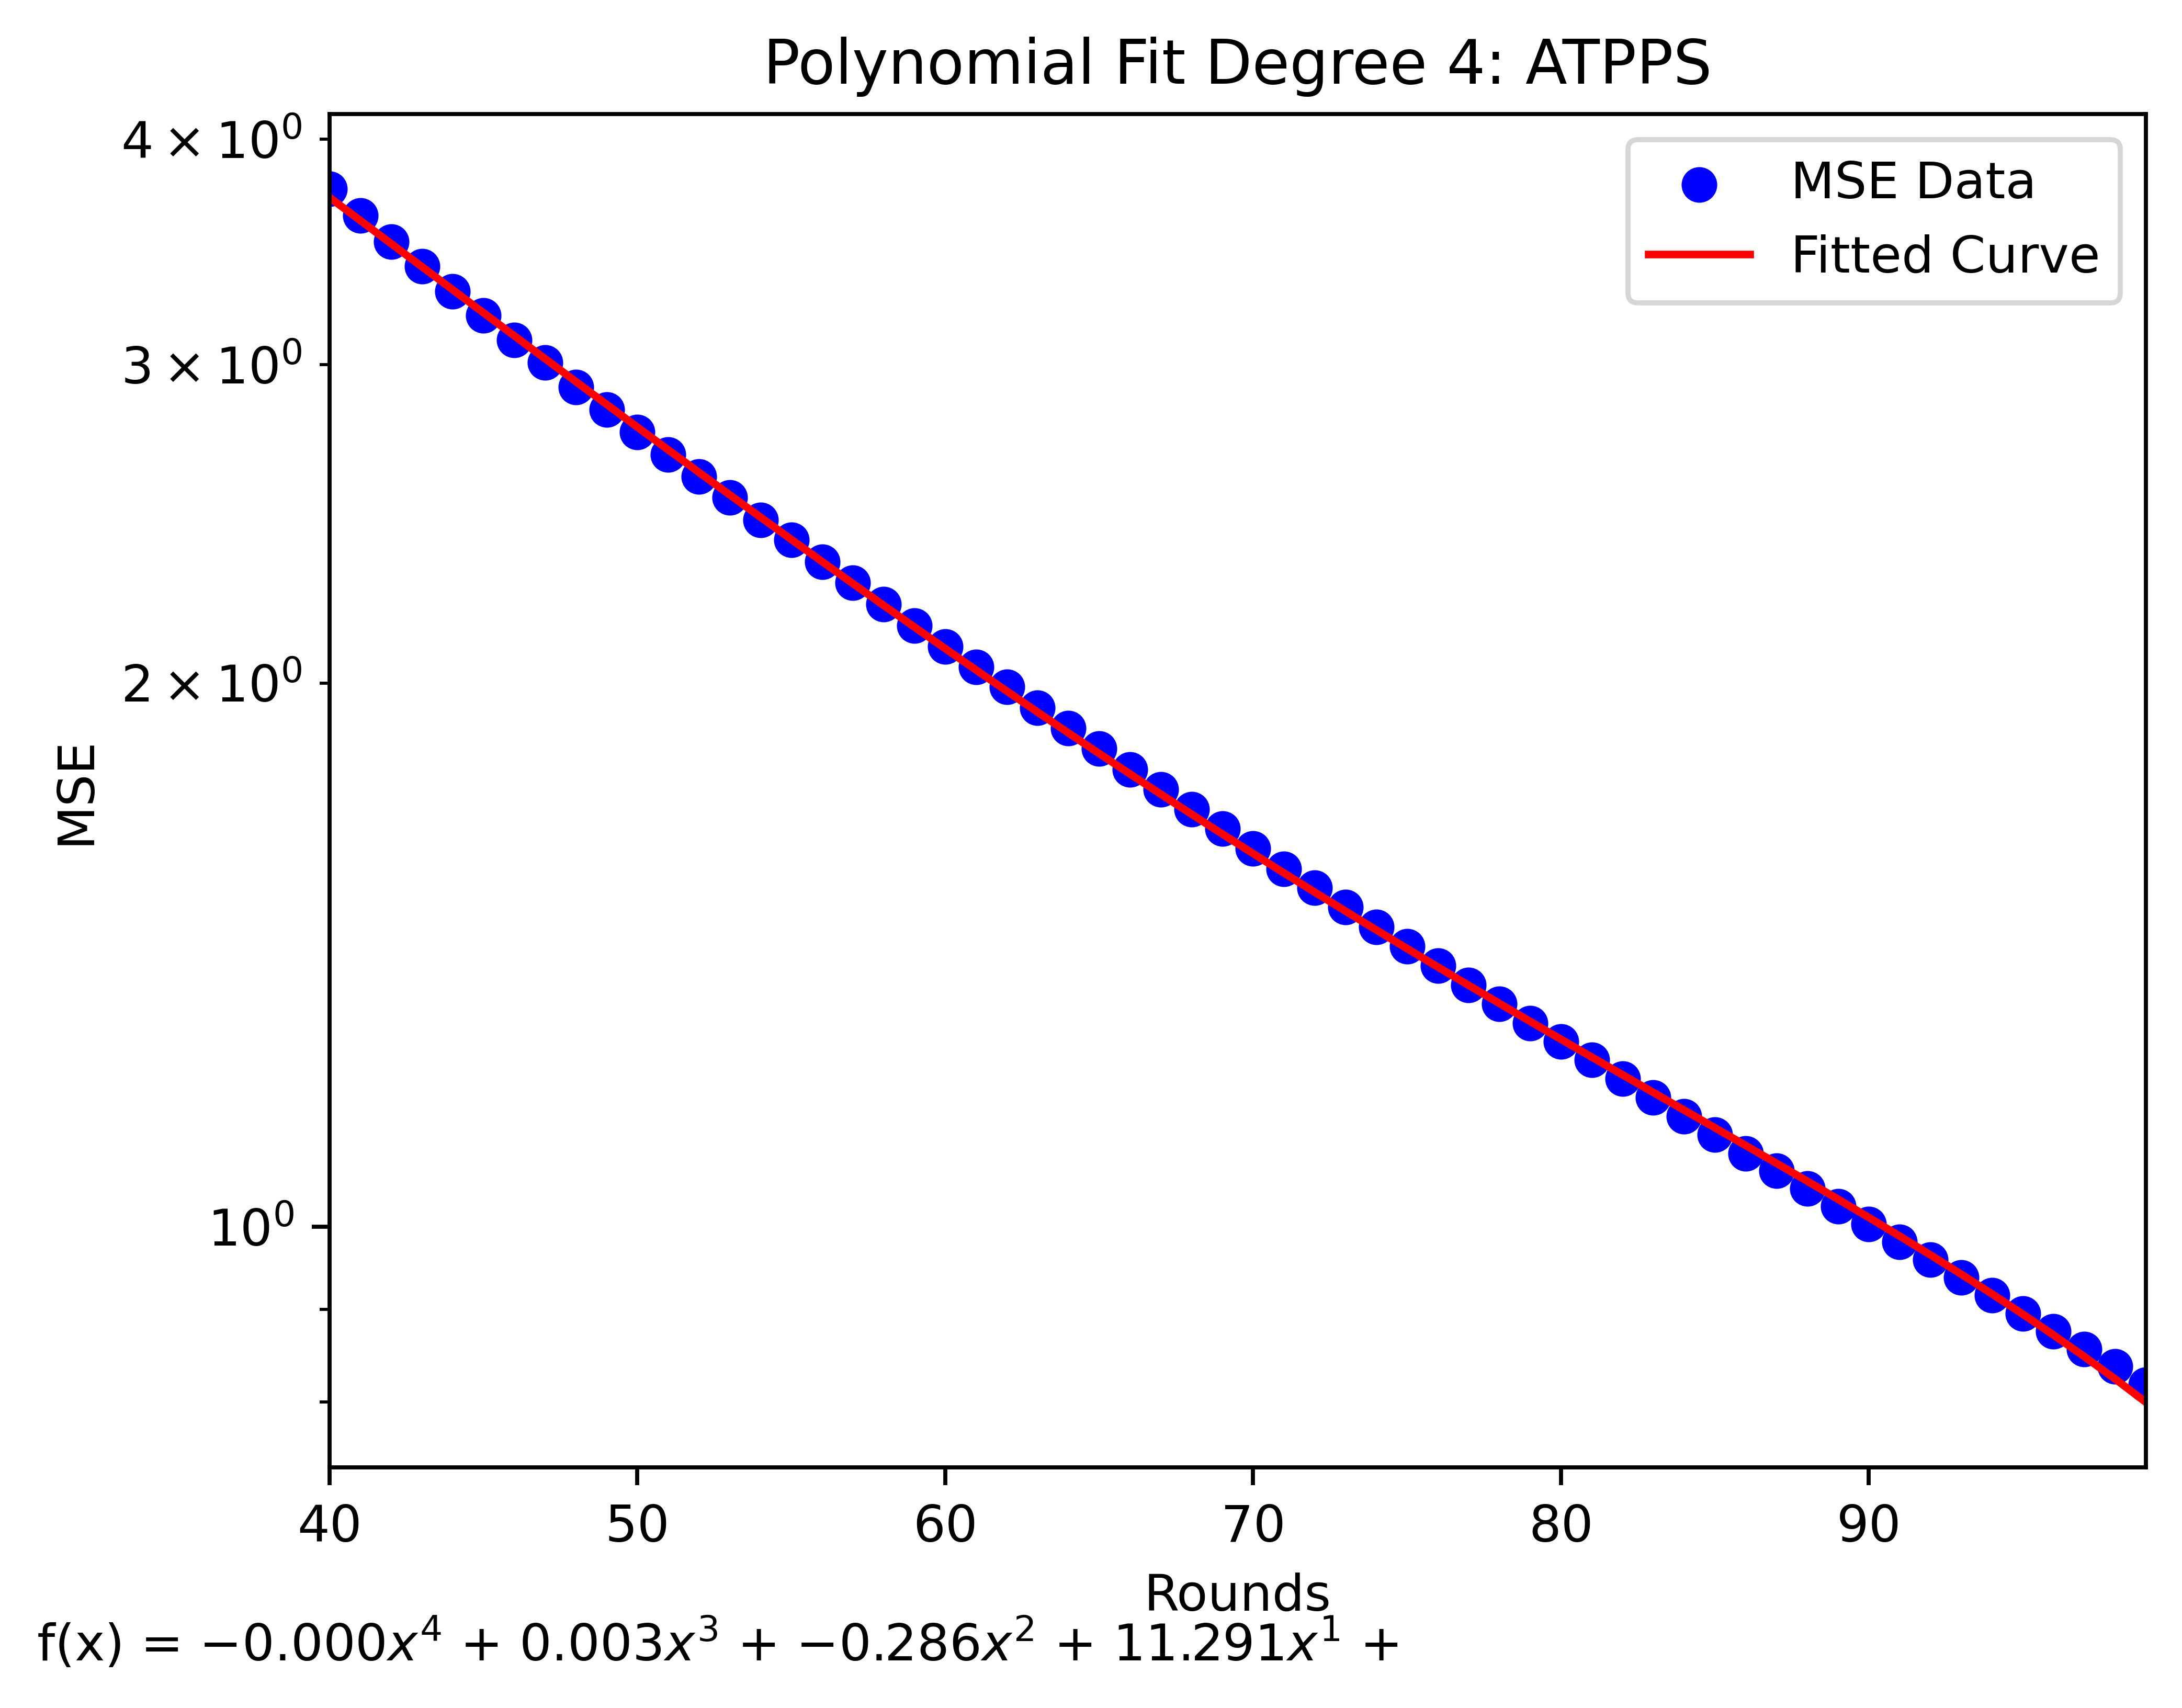
\includegraphics[width=0.49\linewidth]{figures/Simulation_outcomes/TorusGridGraph/ATPPS/ATPPS_modelfitting_rounds_99_model_2.png}}
%    \caption{Polynomial Regression Fit: ATPPS; Rounds 10-39 and 40-100}
%        \label{fig:atppstorusModelFit}
%\end{figure}

% \begin{figure}
%     \centering
%     \scalebox{0.8}{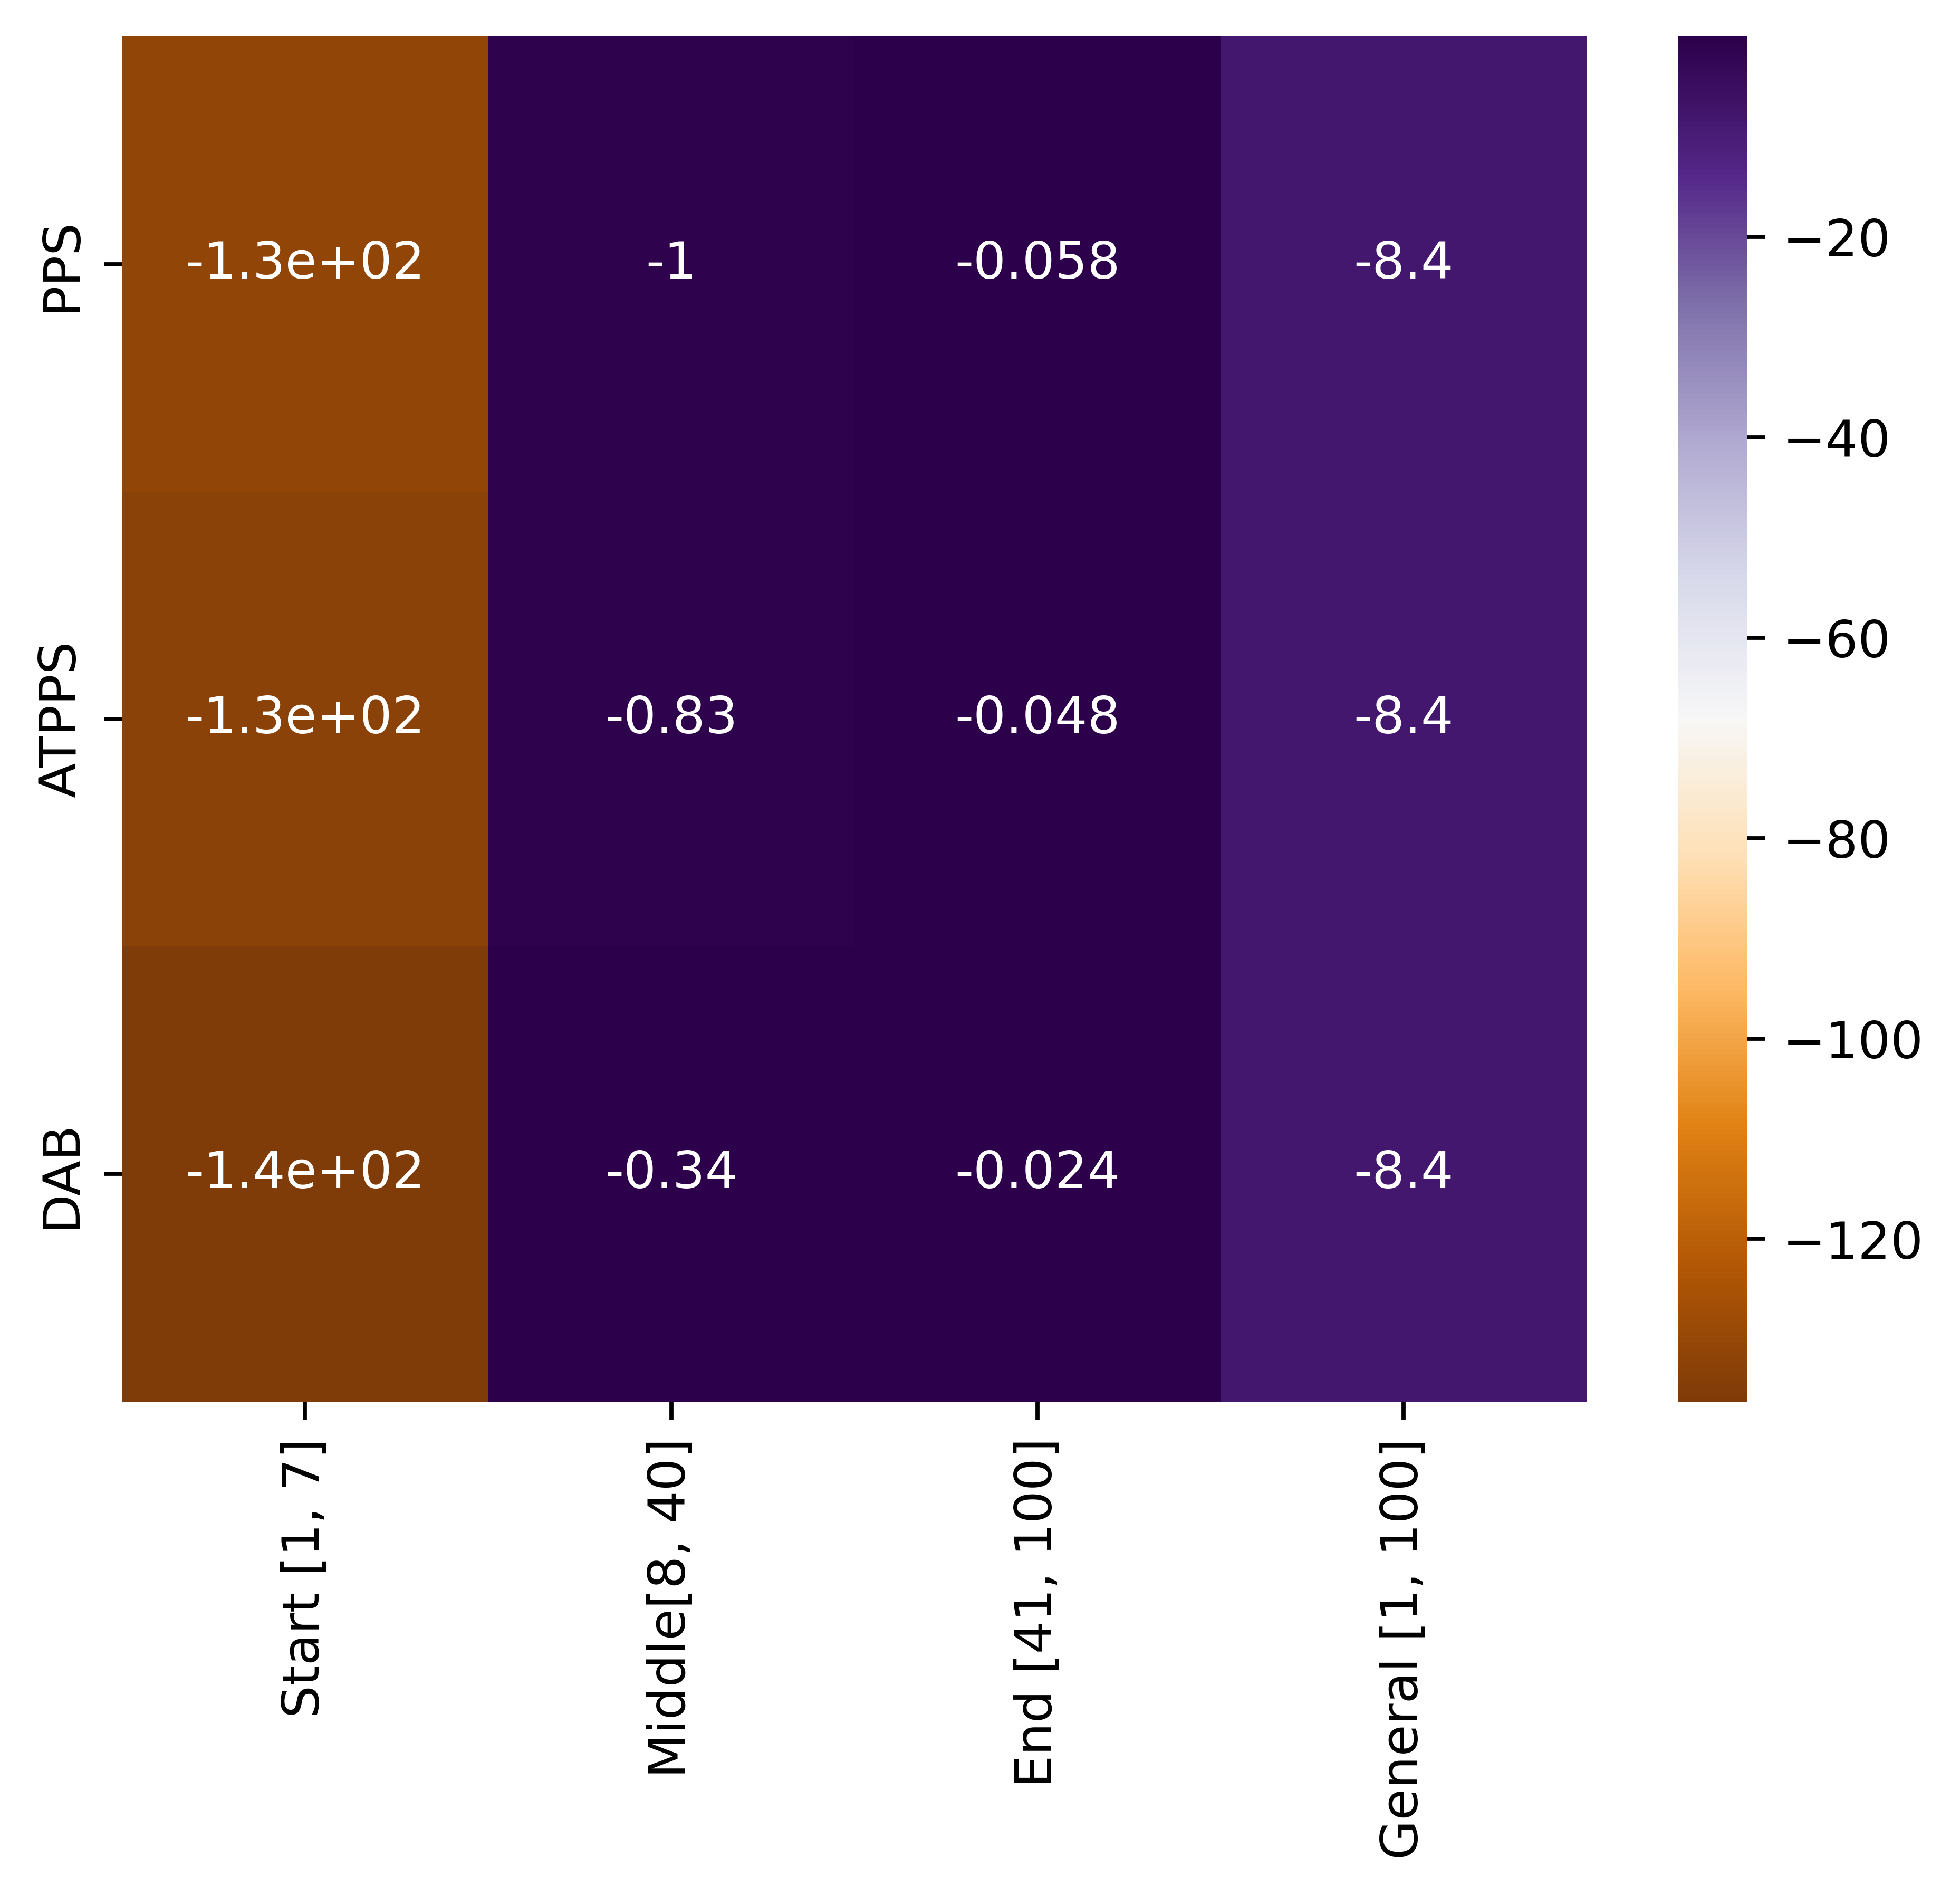
\includegraphics{figures/Simulation_outcomes/TorusGridGraph/DAB_vs_PPS_vs_ATPPS_slopesheatmap_100rounds.png}}
%     \caption{Torus Grid Graph: heat map of slopes per region}
%     \label{fig:torusgraphslopes}
% \end{figure}


\section{Ring of Cliques}\label{sec:ringofcliques}
In the early rounds, PPS and ATPPS exhibits the fastest MSE reduction showcased by a very steep downwards trend between rounds 1 and 5 in figure \ref{fig:atppsRingOfCliquesLog_LogLog} a). Both PPS-based approaches start with faster convergence rates compared to DAB. The initial steep downwards slope of -200 for each PPS-based algorithm as depicted in figure \ref{fig:ringOfCliquesslopes} within the first 5 rounds is due to the unbalanced state of each clique. The PPS-based approaches has shown to be outperforming the DAB algorithm for complete graphs. While the Cliques are still unbalanced the PPS-based algorithms achieve faster convergence. After the cliques are balanced round by round the DAB algorithm catches up especially between the rounds 6 to 40 where the slopes seem to be -48 compared to $\sim-2$ for the PPS-based algorithms.  Nodes within cliques tend to converge quickly internally due to their dense interconnections for the PPS-based algorithms. However, load balancing between cliques, especially when the nodes select for random neighbors is slower, creating bottlenecks for global convergence. Due to the determistic nature of the DAB, the bridging nodes choose nodes outside of their cliques, once the load is balanced within the clique, and spread the load to other cliques. The ATPPS algorithm achieves better results compared to the PPS, since it has a similar mechanism in this scenario like the DAB. In the Ring of Cliques, this mechanism prioritizes communication between cliques (where differences in loads are more significant) over redundant communication within cliques (where loads are already close to balanced). This helps speed up inter-clique convergence. And so it acts as a compromise solution between the PPS and the DAB again achieving results close to them of the DAB algorithm.

The polynomial fit for the DAB algorithm is: $MSE_r=1.04\times 10^{-6}r^{4}-2.941\times 10^{-4}r^{3}+0.03r^{2}-1.66r+45.30$. Thus the Mean Squared Error (MSE) as a function of rounds is modeled by a fourth-degree polynomial. The PPS MSE data of rounds 20 to 100 is fitted to a linear regression model following the equation: $MSE_r=-0.05r+24.70$. The negative slope indicates a consistent reduction in MSE with each round in this region, but the value -0.05 is relatively small. This suggests that the PPS algorithm achieves slow and steady progress toward load balancing. The linear fit highlights that PPS achieves only gradual improvement in balancing the load in the Ring of Cliques topology. This is because:

PPS focuses on a push-pull mechanism that is inherently less targeted, relying on random neighbor interactions.
In the Ring of Cliques, inter-clique connections are sparse, and PPS lacks a mechanism to prioritize balancing between these sparsely connected regions. As a result, its performance is bottlenecked by the topology. The linearity of the model suggests a uniform rate of error reduction across rounds, without any acceleration observed in other methods (like DAB). The logarithmic model for the ATPPS algorithm is given as:
$\log{(MSE_r)}=-7.59\log{(r)}+43.26$. By exponentiating this equation, the relationship between the Mean Squared Error and the number of rounds is: $MSE_r=10^{43.26}*r-7.59$. The steep negative slope with value -7.59 in the log-log fit indicates a rapid decrease in MSE as the number of rounds increases. This suggests that ATPPS achieves exponentially faster convergence compared to PPS, especially in the early rounds of load balancing.

%\begin{figure}[!ht]
%    \centering
%        \subfloat[]{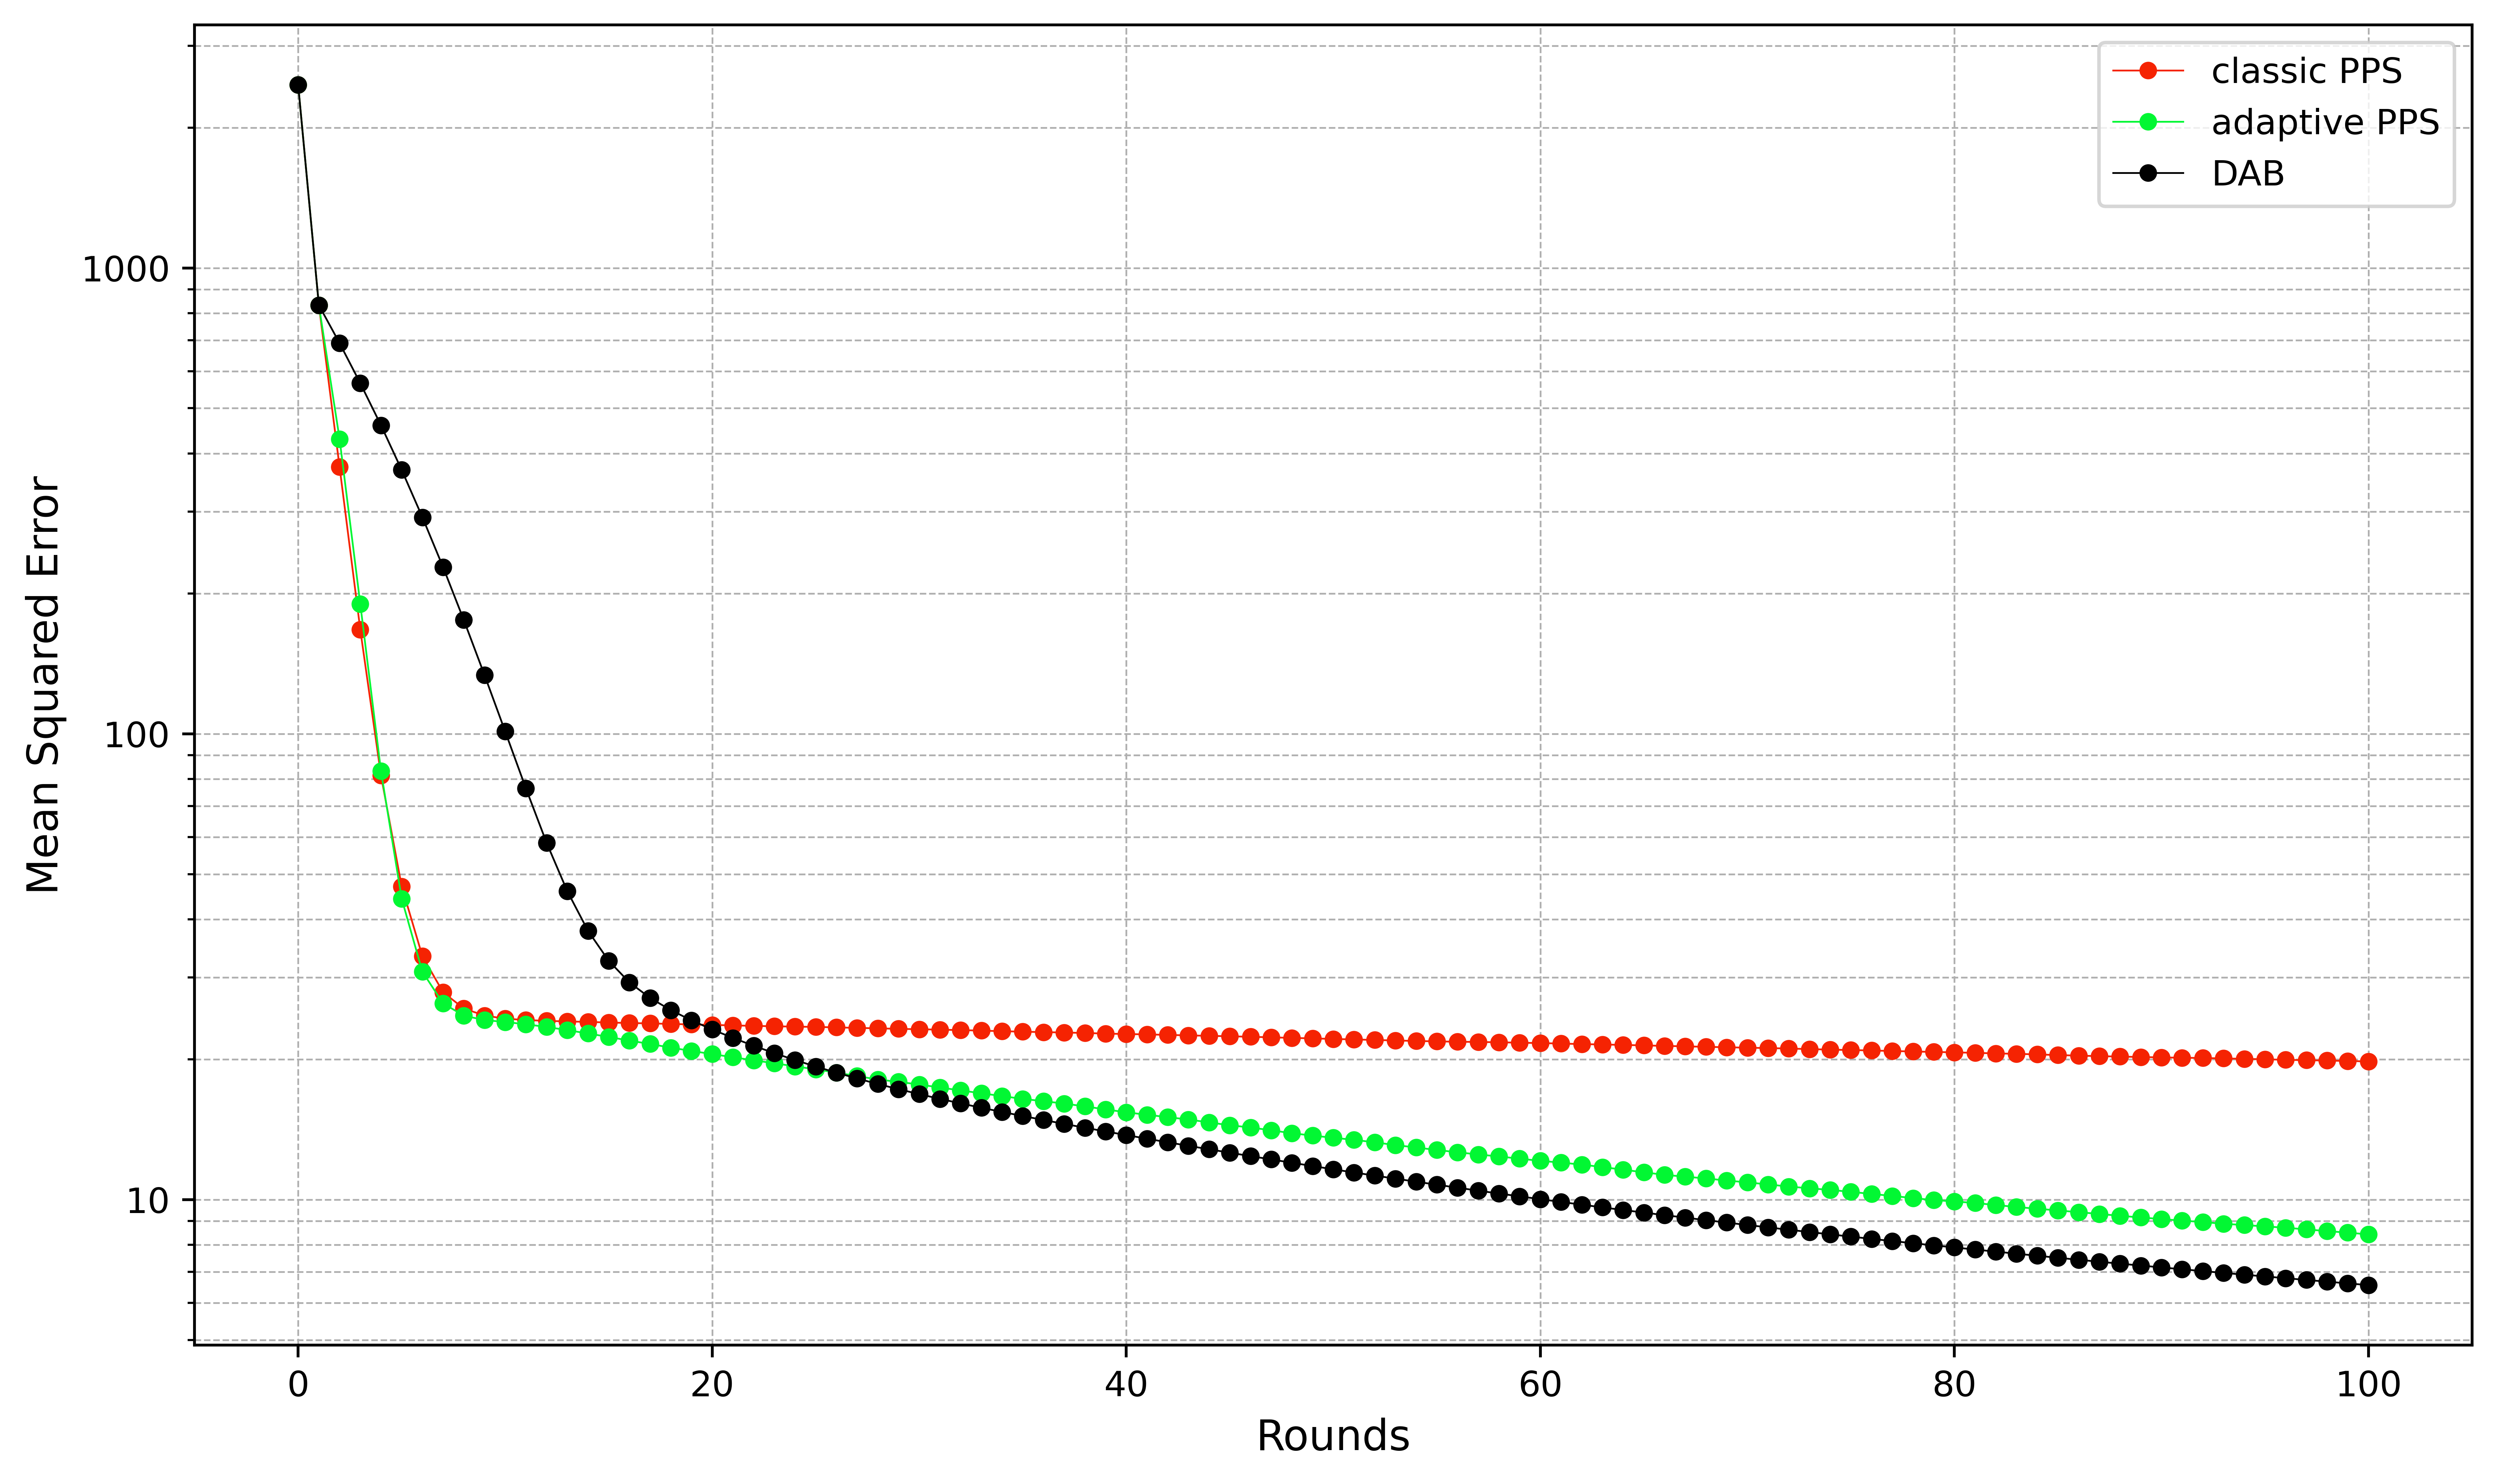
\includegraphics[width=0.49\linewidth]{figures/Simulation_outcomes/RingOfCliques/DAB_vs_PPS_RoC_r100_n1024_averaged_log.png}}
%    \hfil
%        \subfloat[]{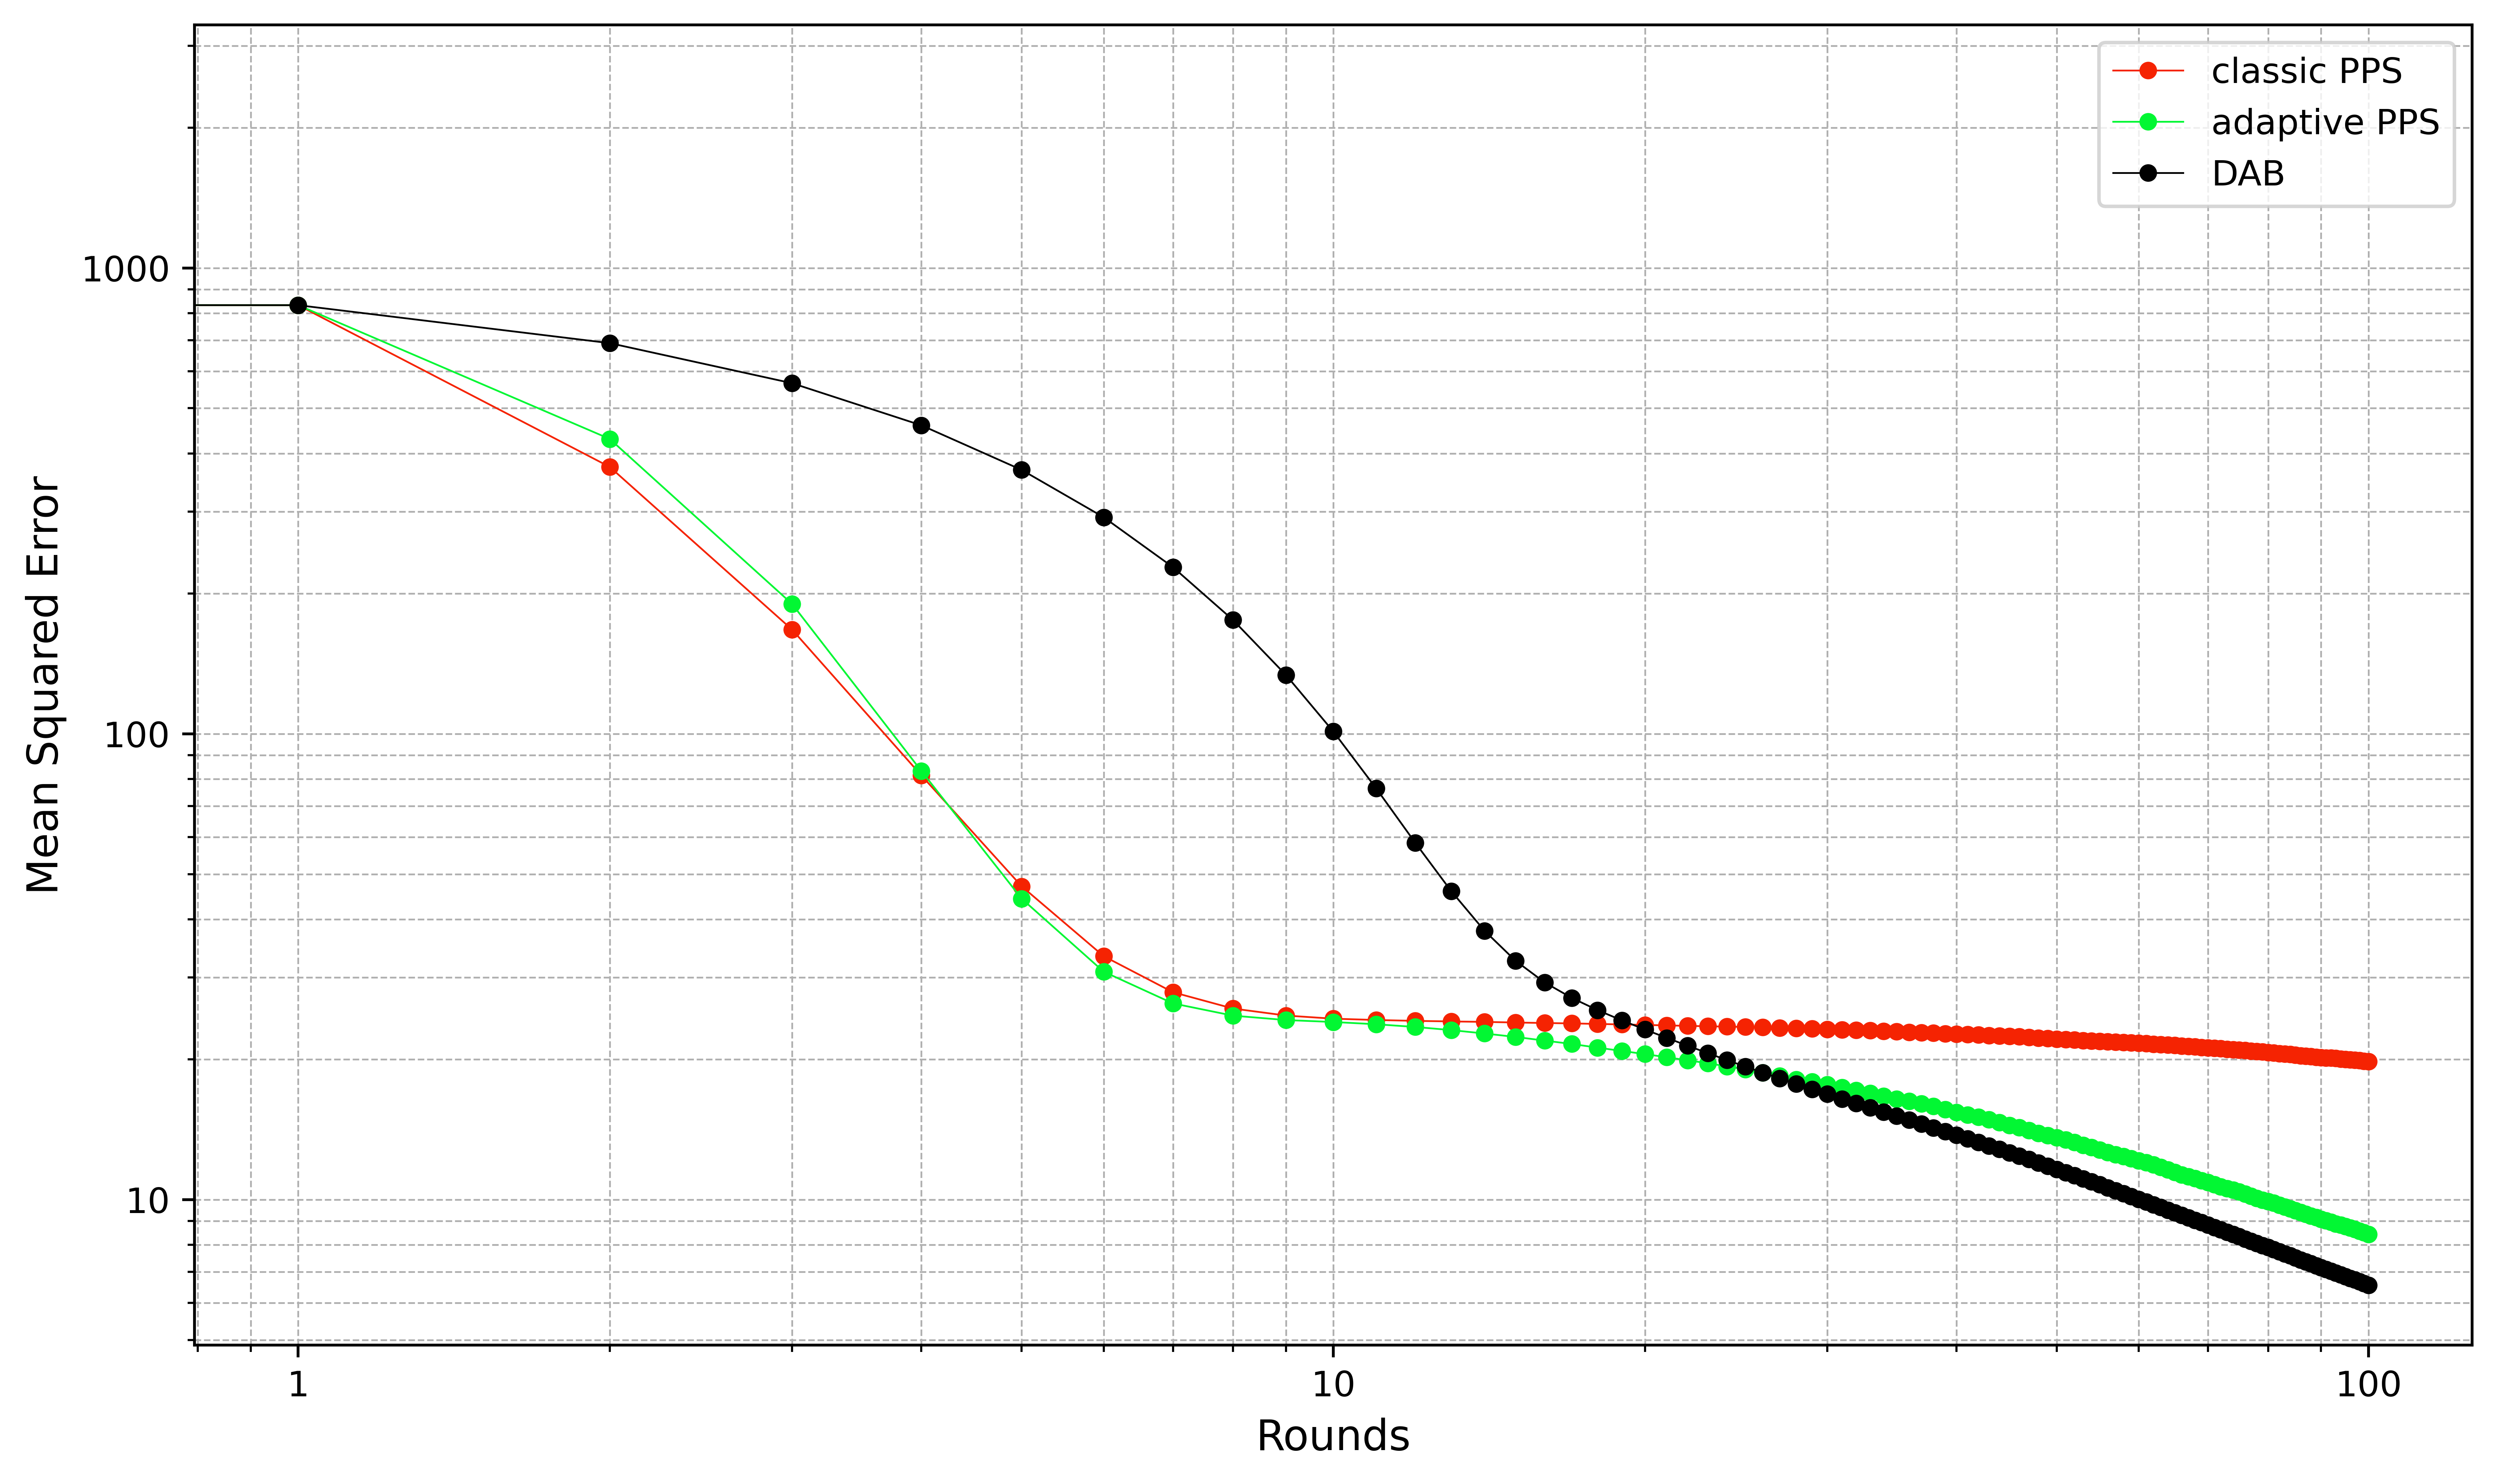
\includegraphics[width=0.49\linewidth]{figures/Simulation_outcomes/RingOfCliques/DAB_vs_PPS_RoC_r100_n1024_averaged_loglog.png}}
%    \caption{Ring of Cliques: mean squared error per rounds (left: log-linear; right: log-log)}
%        \label{fig:atppsRingOfCliquesLog_LogLog}
%\end{figure}

%^ \begin{figure}[H]
%^     \centering
%^     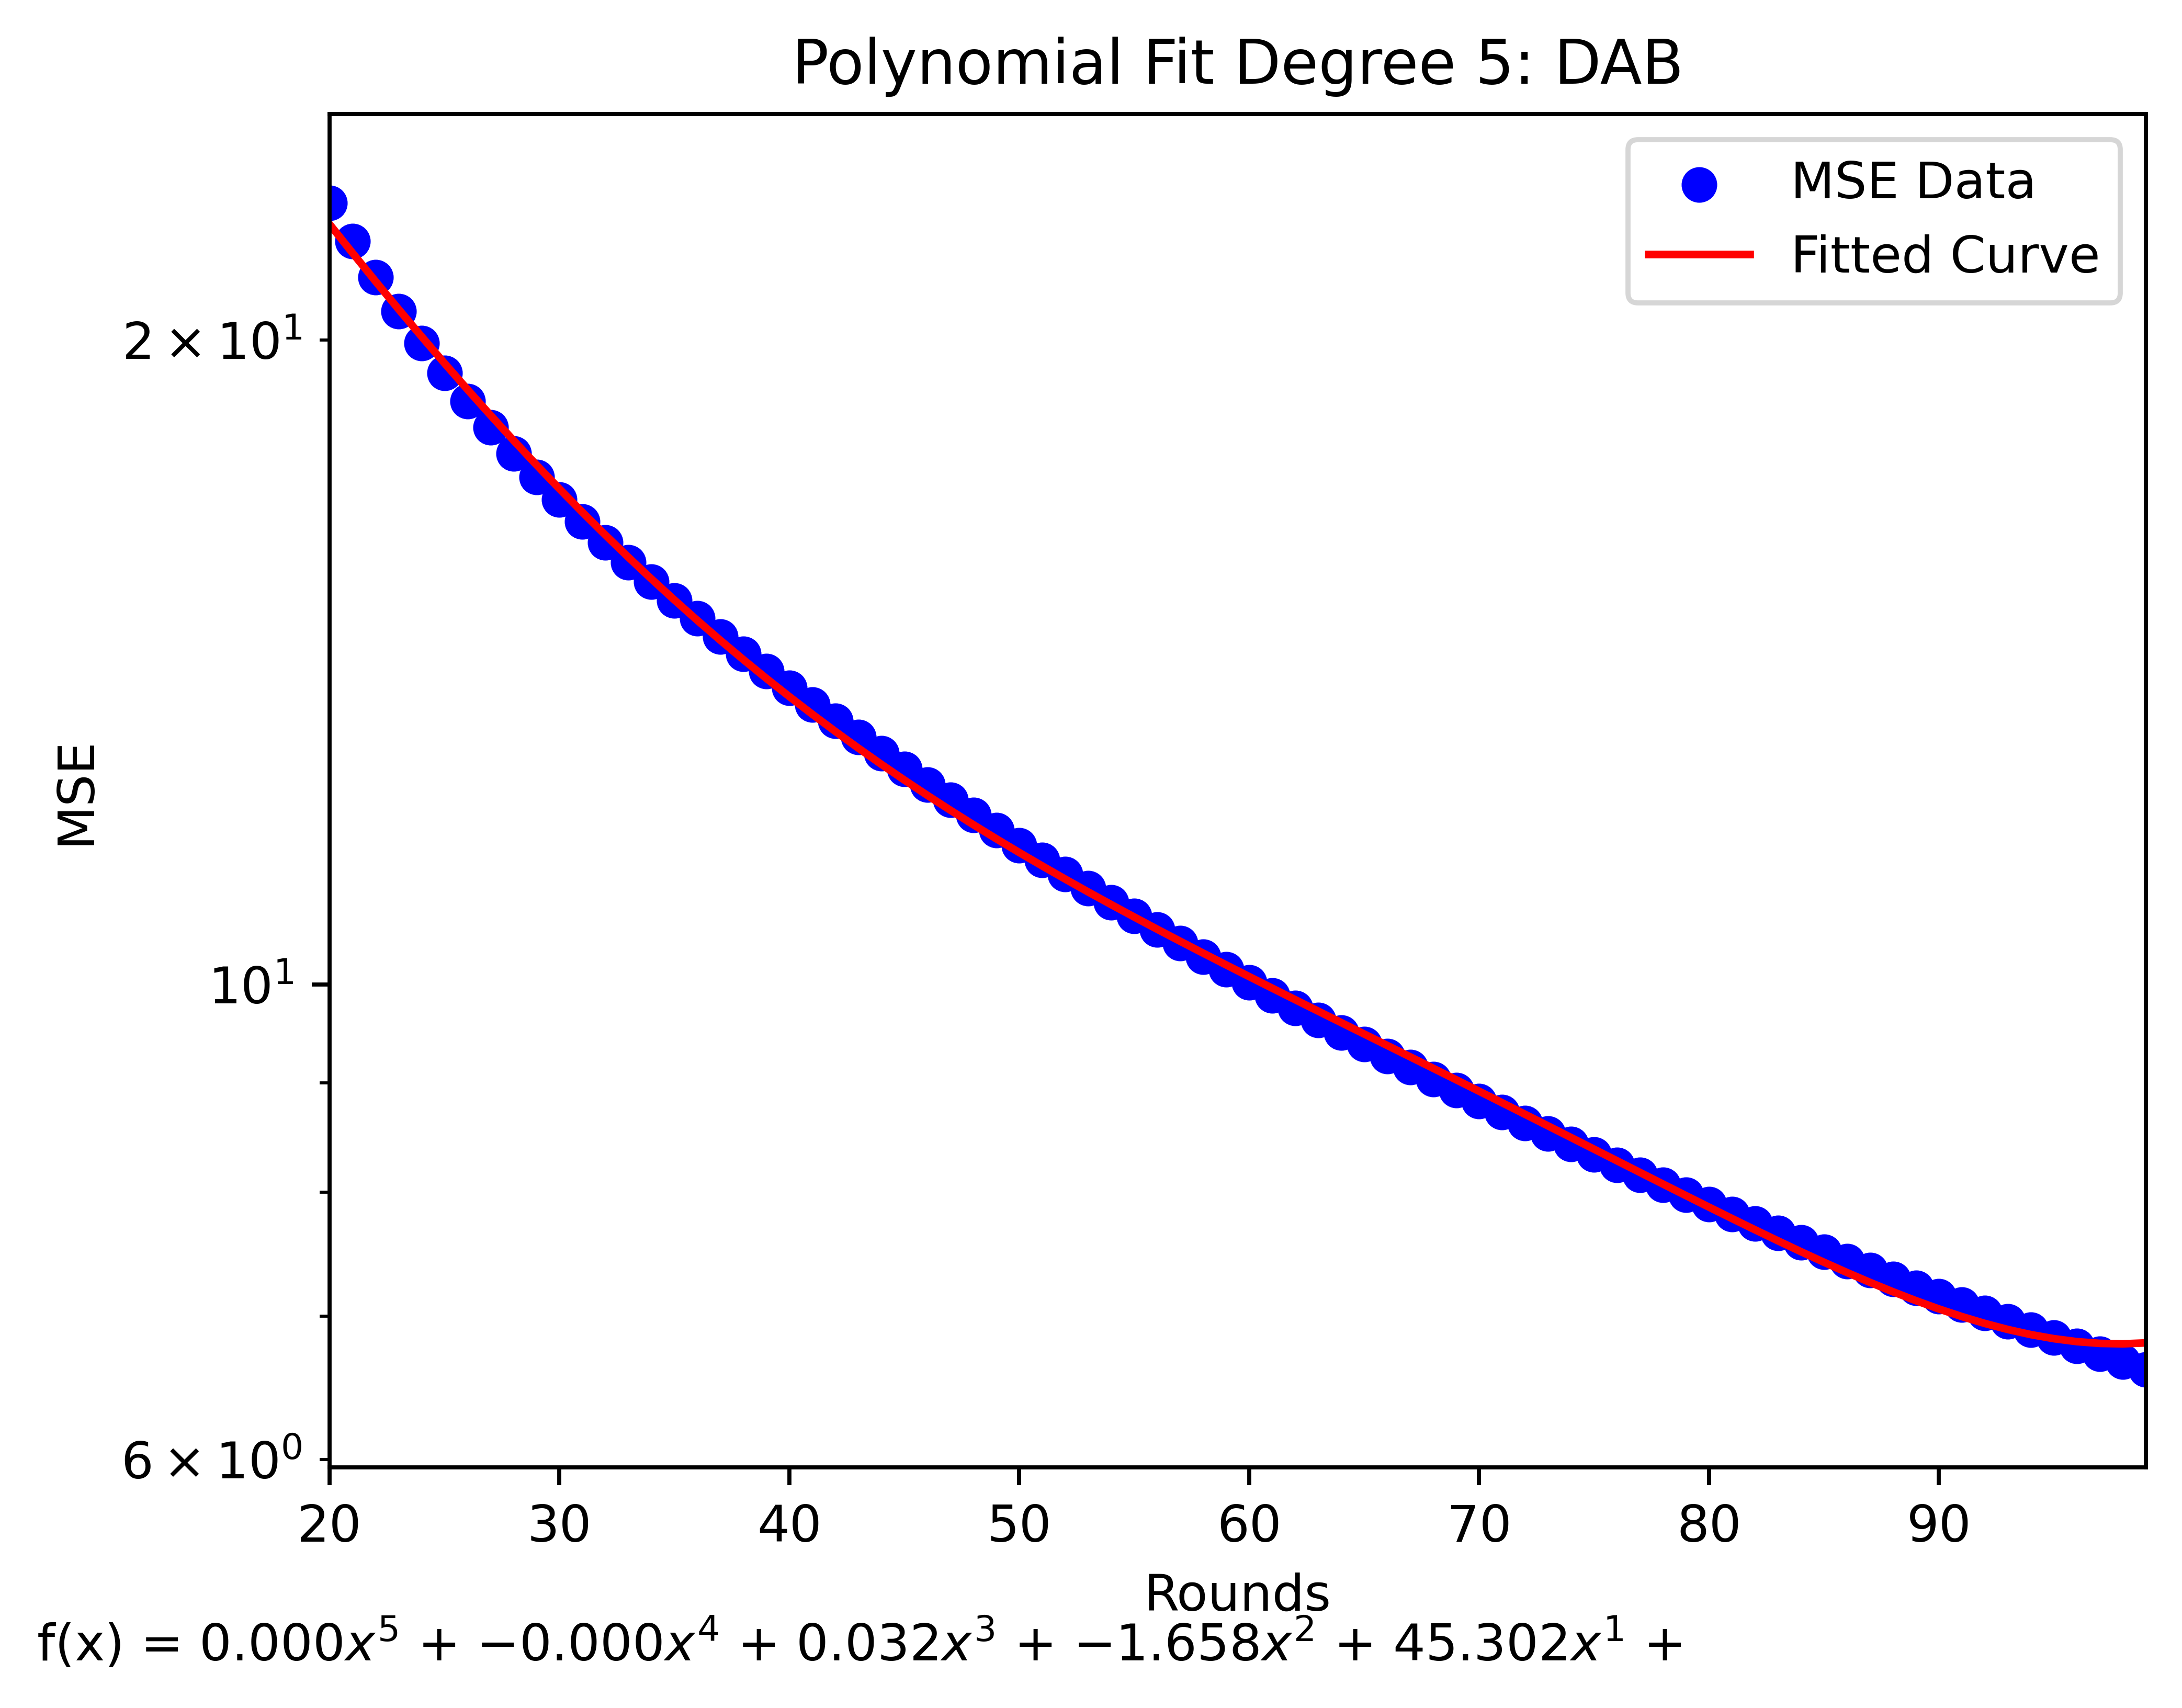
\includegraphics[width=\linewidth]{figures/Simulation_outcomes/RingOfCliques/DAB/DAB_modelfitting_rounds_99_model_2.png}
%^     \caption{Polynomial Regression Fit: DAB}
%^     \label{fig:dabRingOfCliquesModelFit}
%^ \end{figure}
%^\begin{figure}[H]
%^    \centering
%^    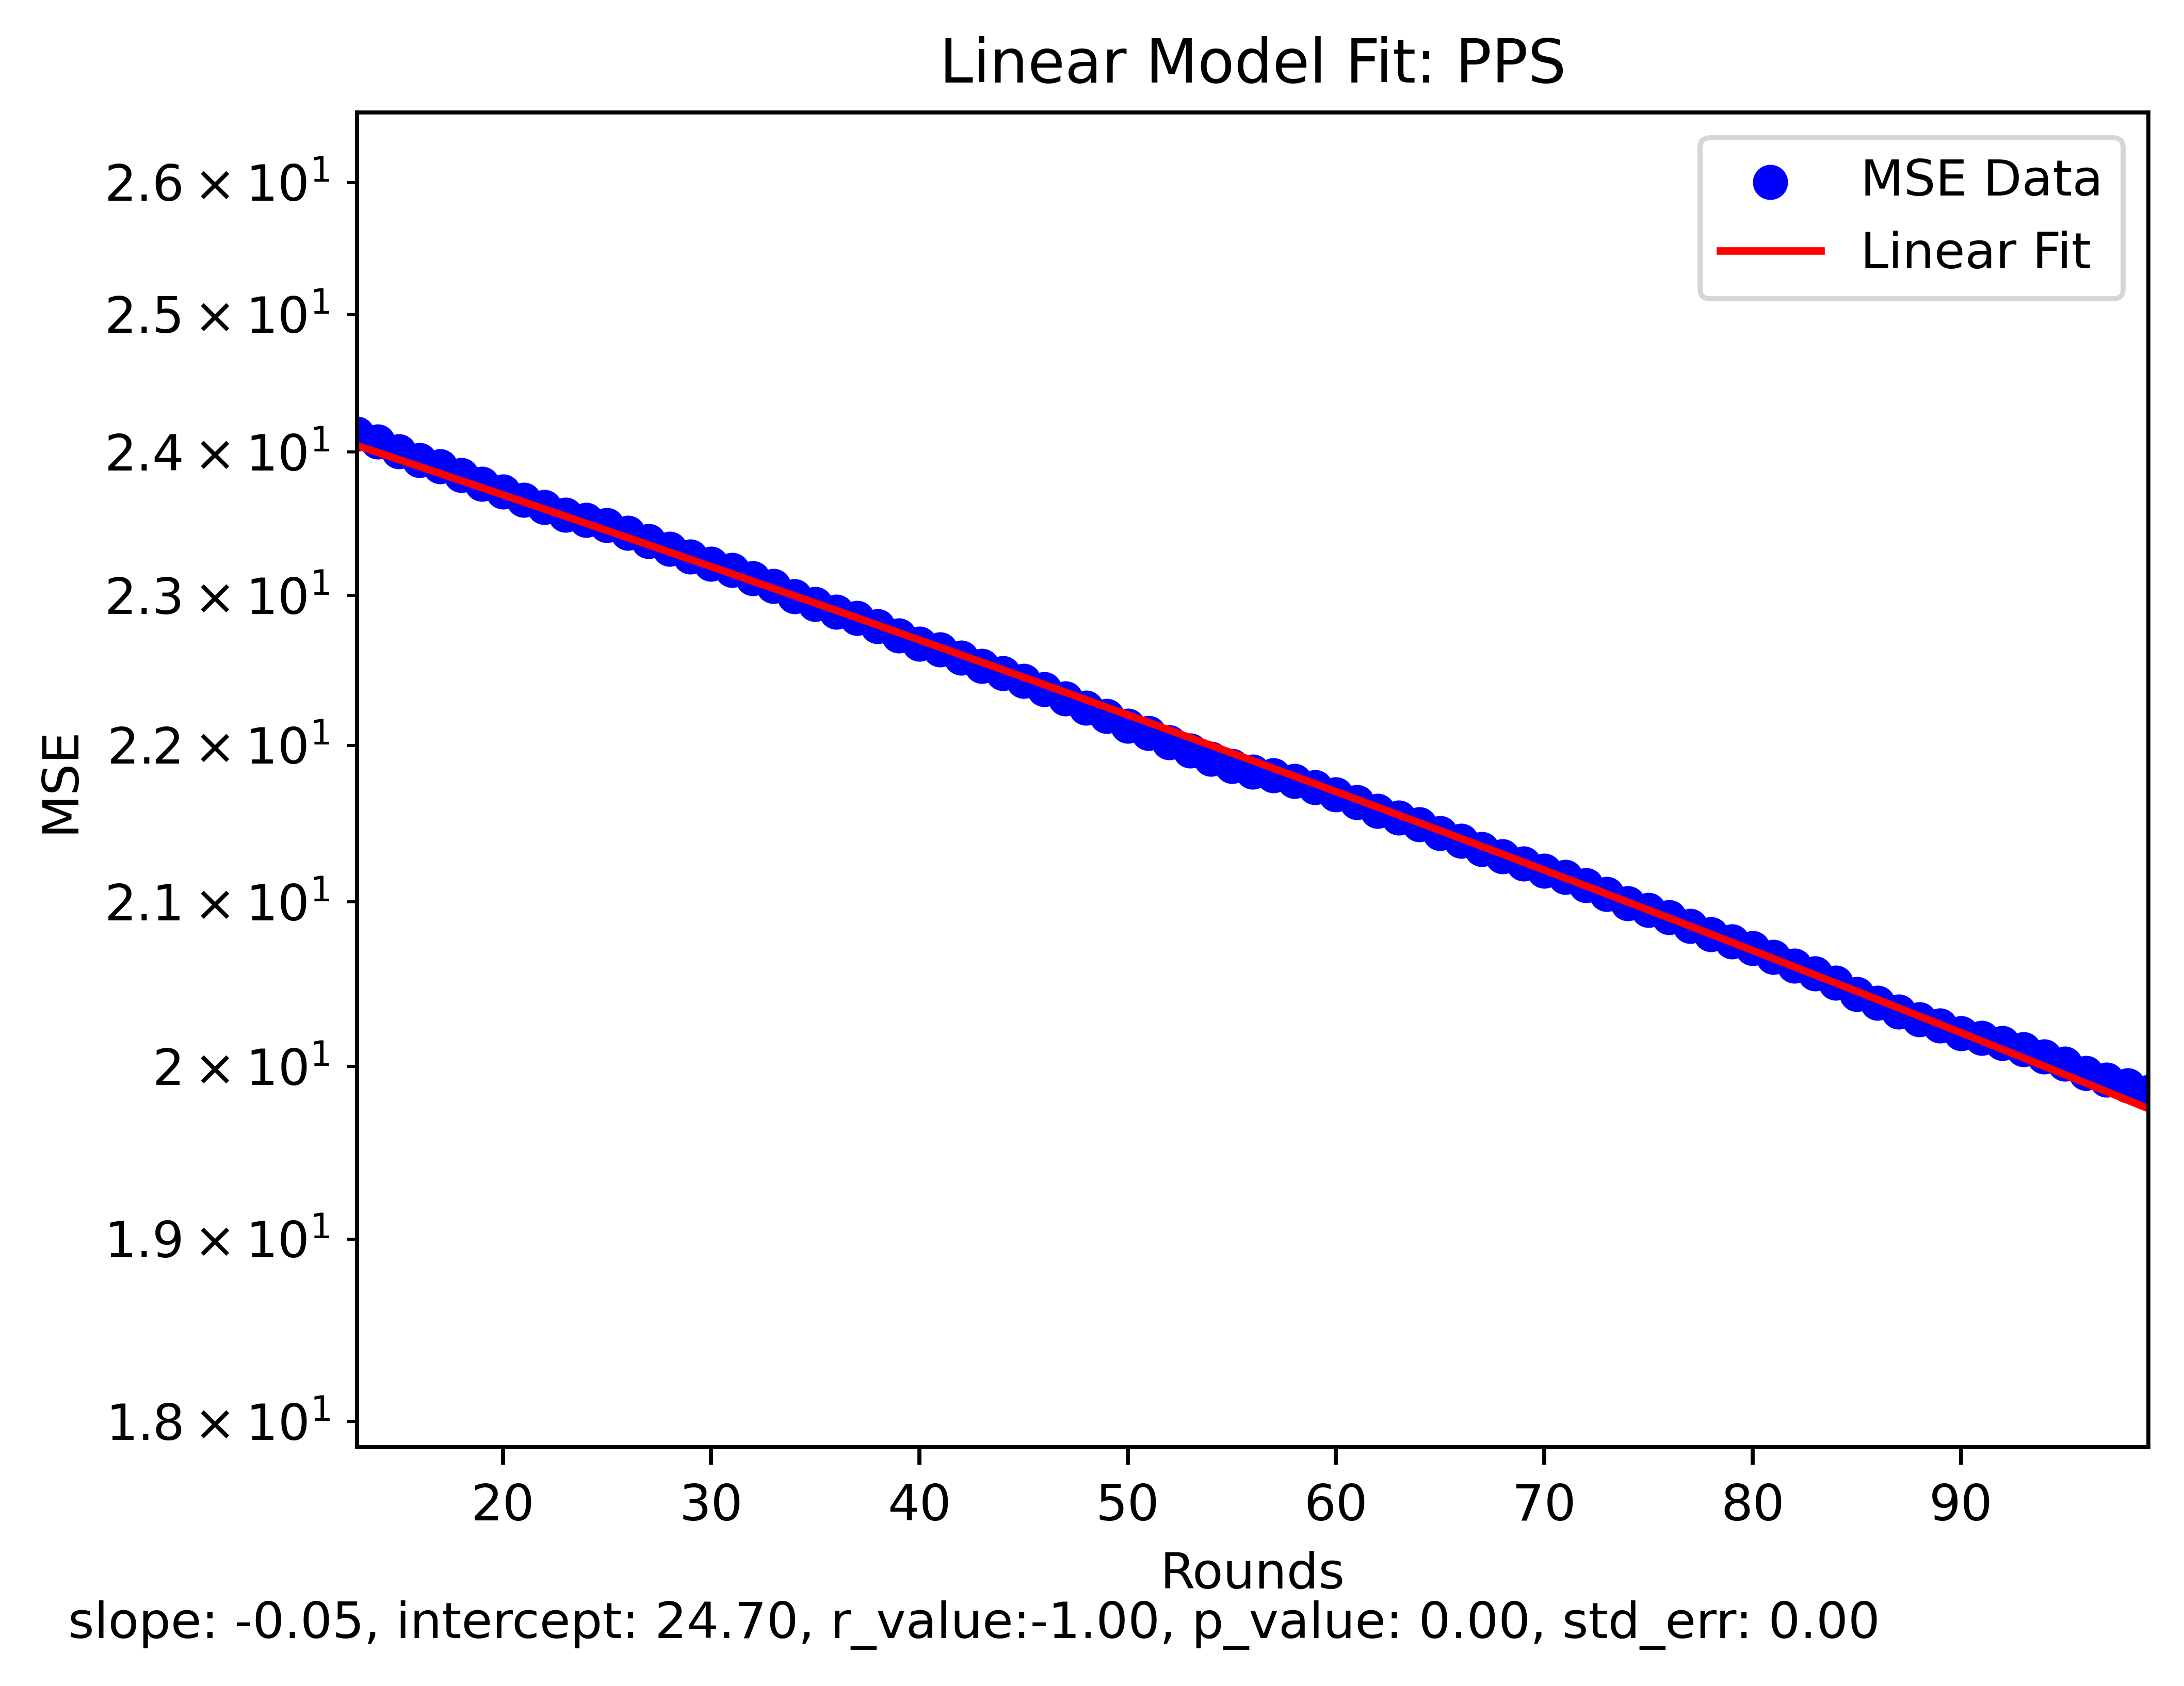
\includegraphics[width=\linewidth]{figures/Simulation_outcomes/RingOfCliques/PPS/PPS_modelfitting_rounds_99_model_0.png}
%^    \caption{Polynomial Regression Fit: PPS}
%^    \label{fig:ppsRingOfCliquesModelFit}
%^\end{figure}
%^
%^\begin{figure}[H]
%^    \centering
%^    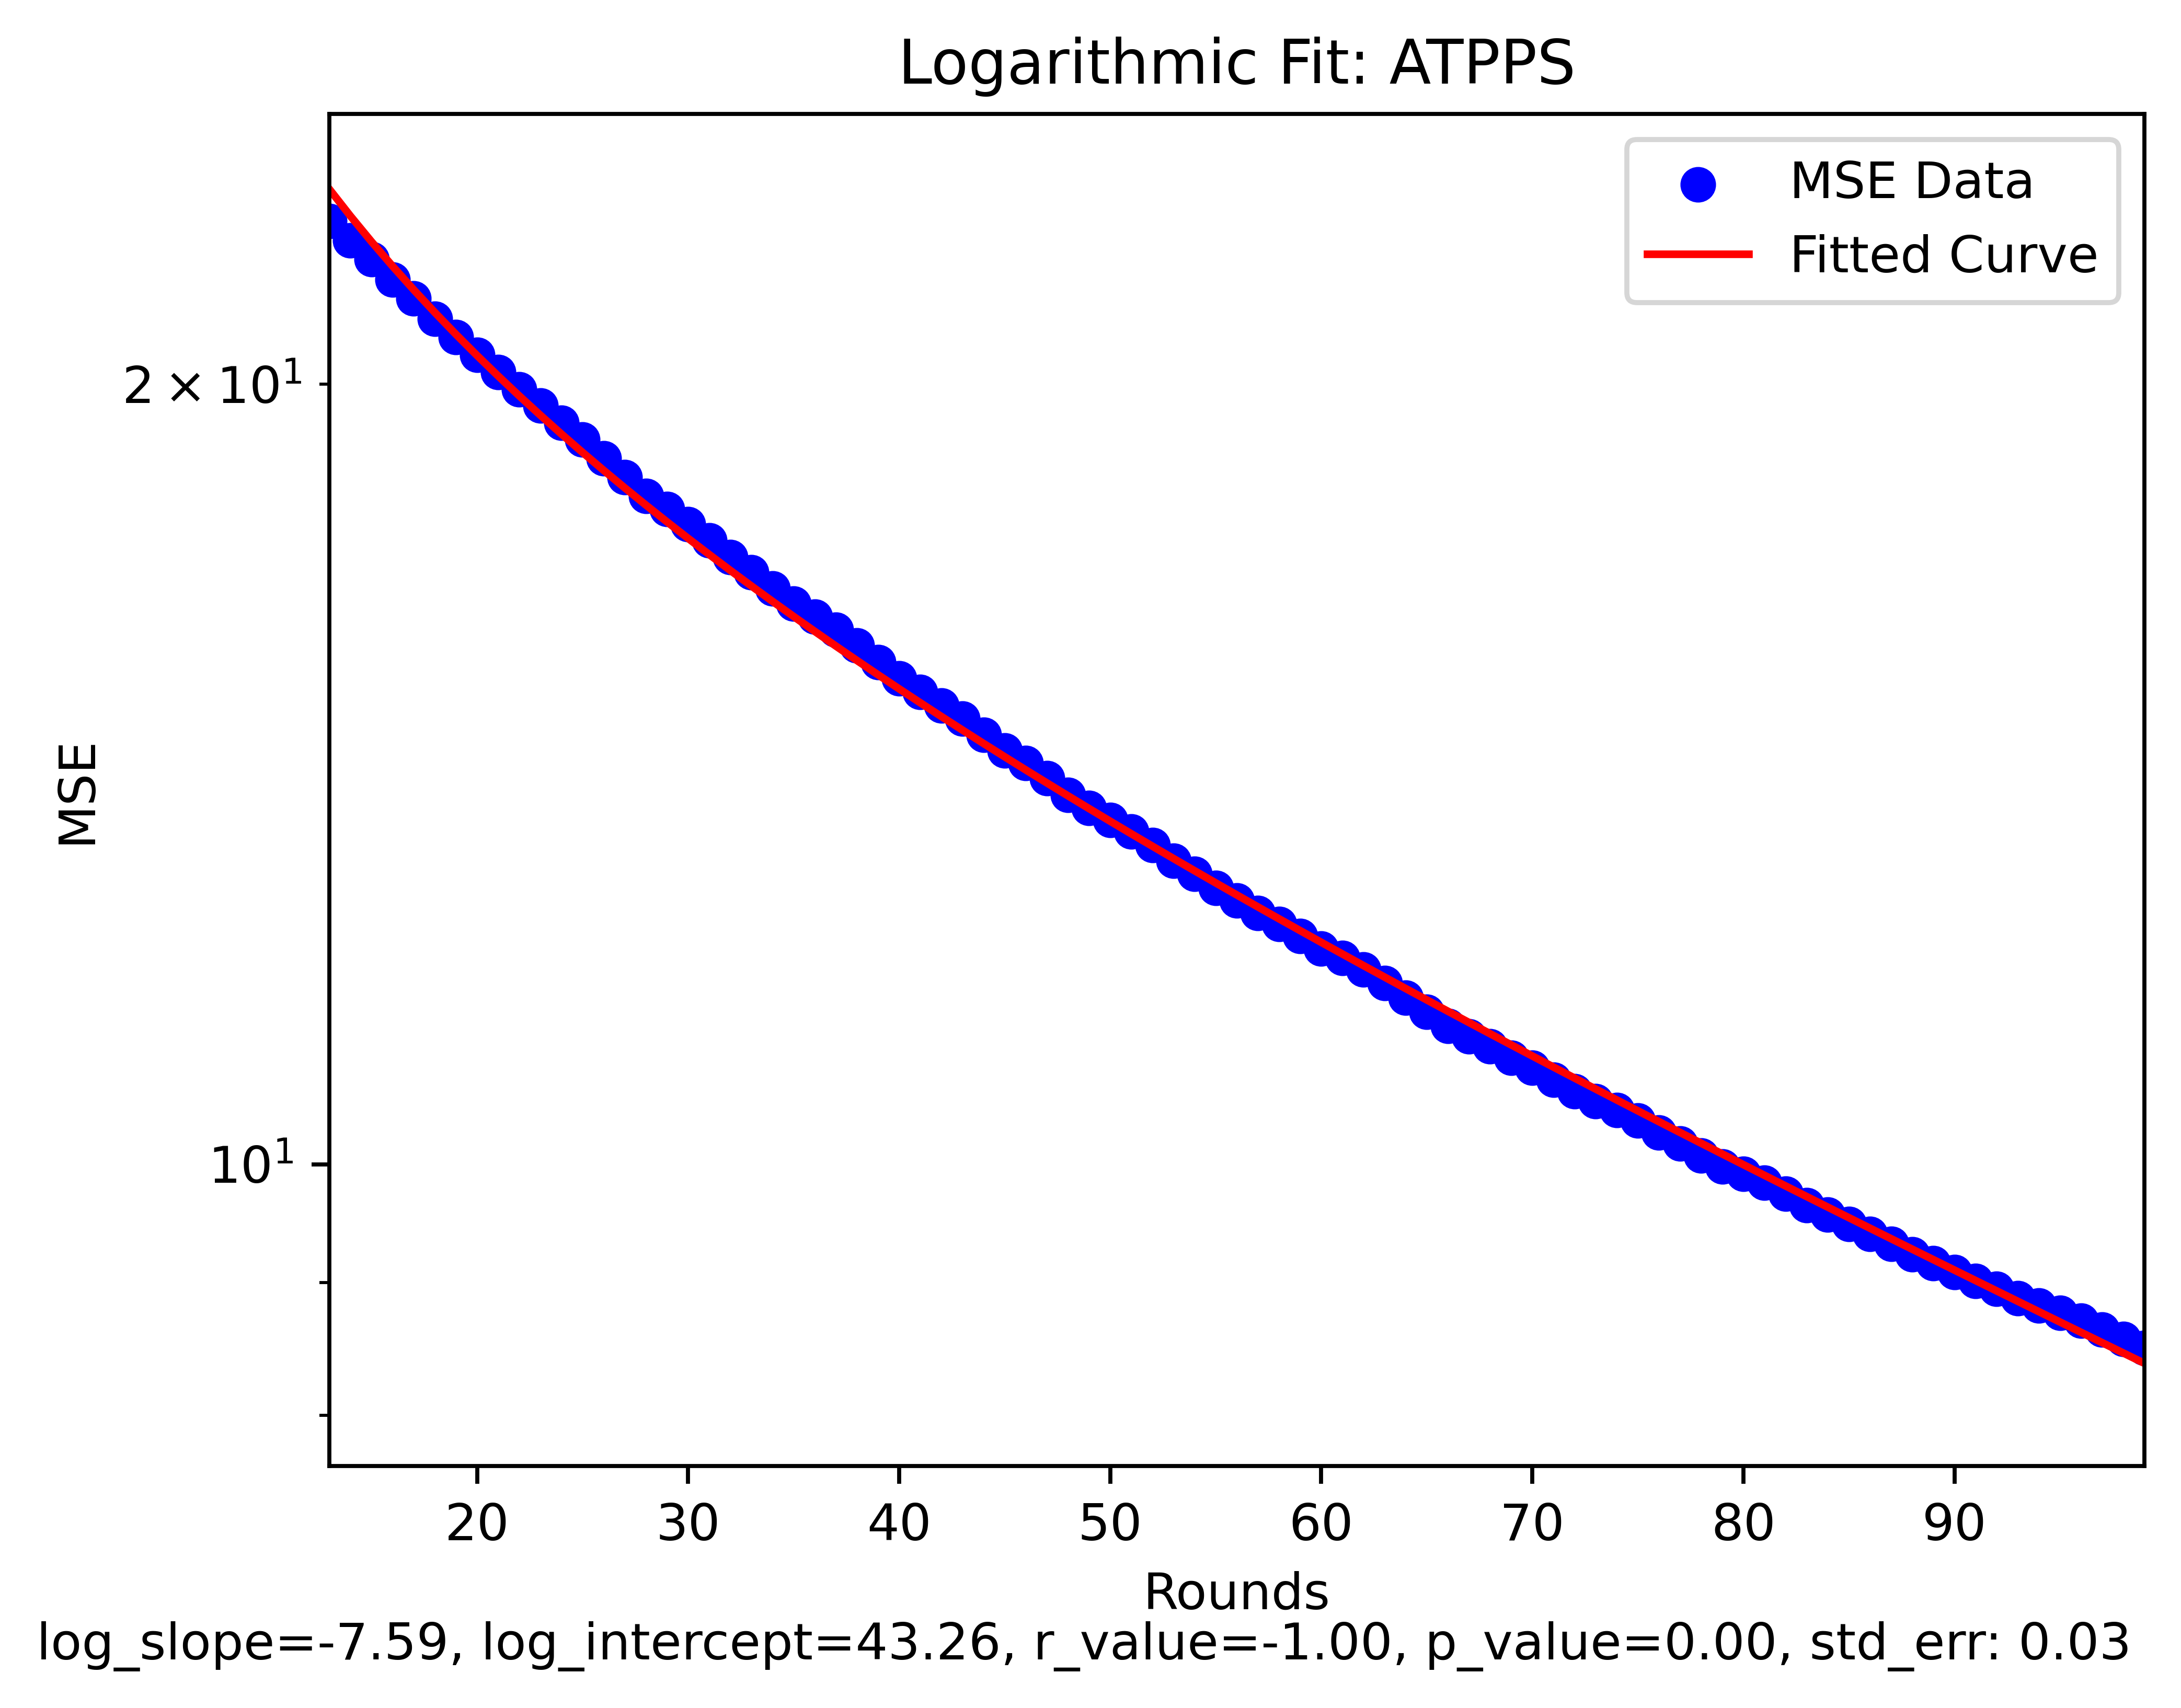
\includegraphics[width=\linewidth]{figures/Simulation_outcomes/RingOfCliques/ATPPS/ATPPS_modelfitting_rounds_99_model_3.png}
%^    \caption{Logarithmic Regression Fit: ATPPS}
%^    \label{fig:atppsRingOfCliquesModelFit}
%^\end{figure}
%^
%^\begin{figure}
%^    \centering
%^    \scalebox{0.8}{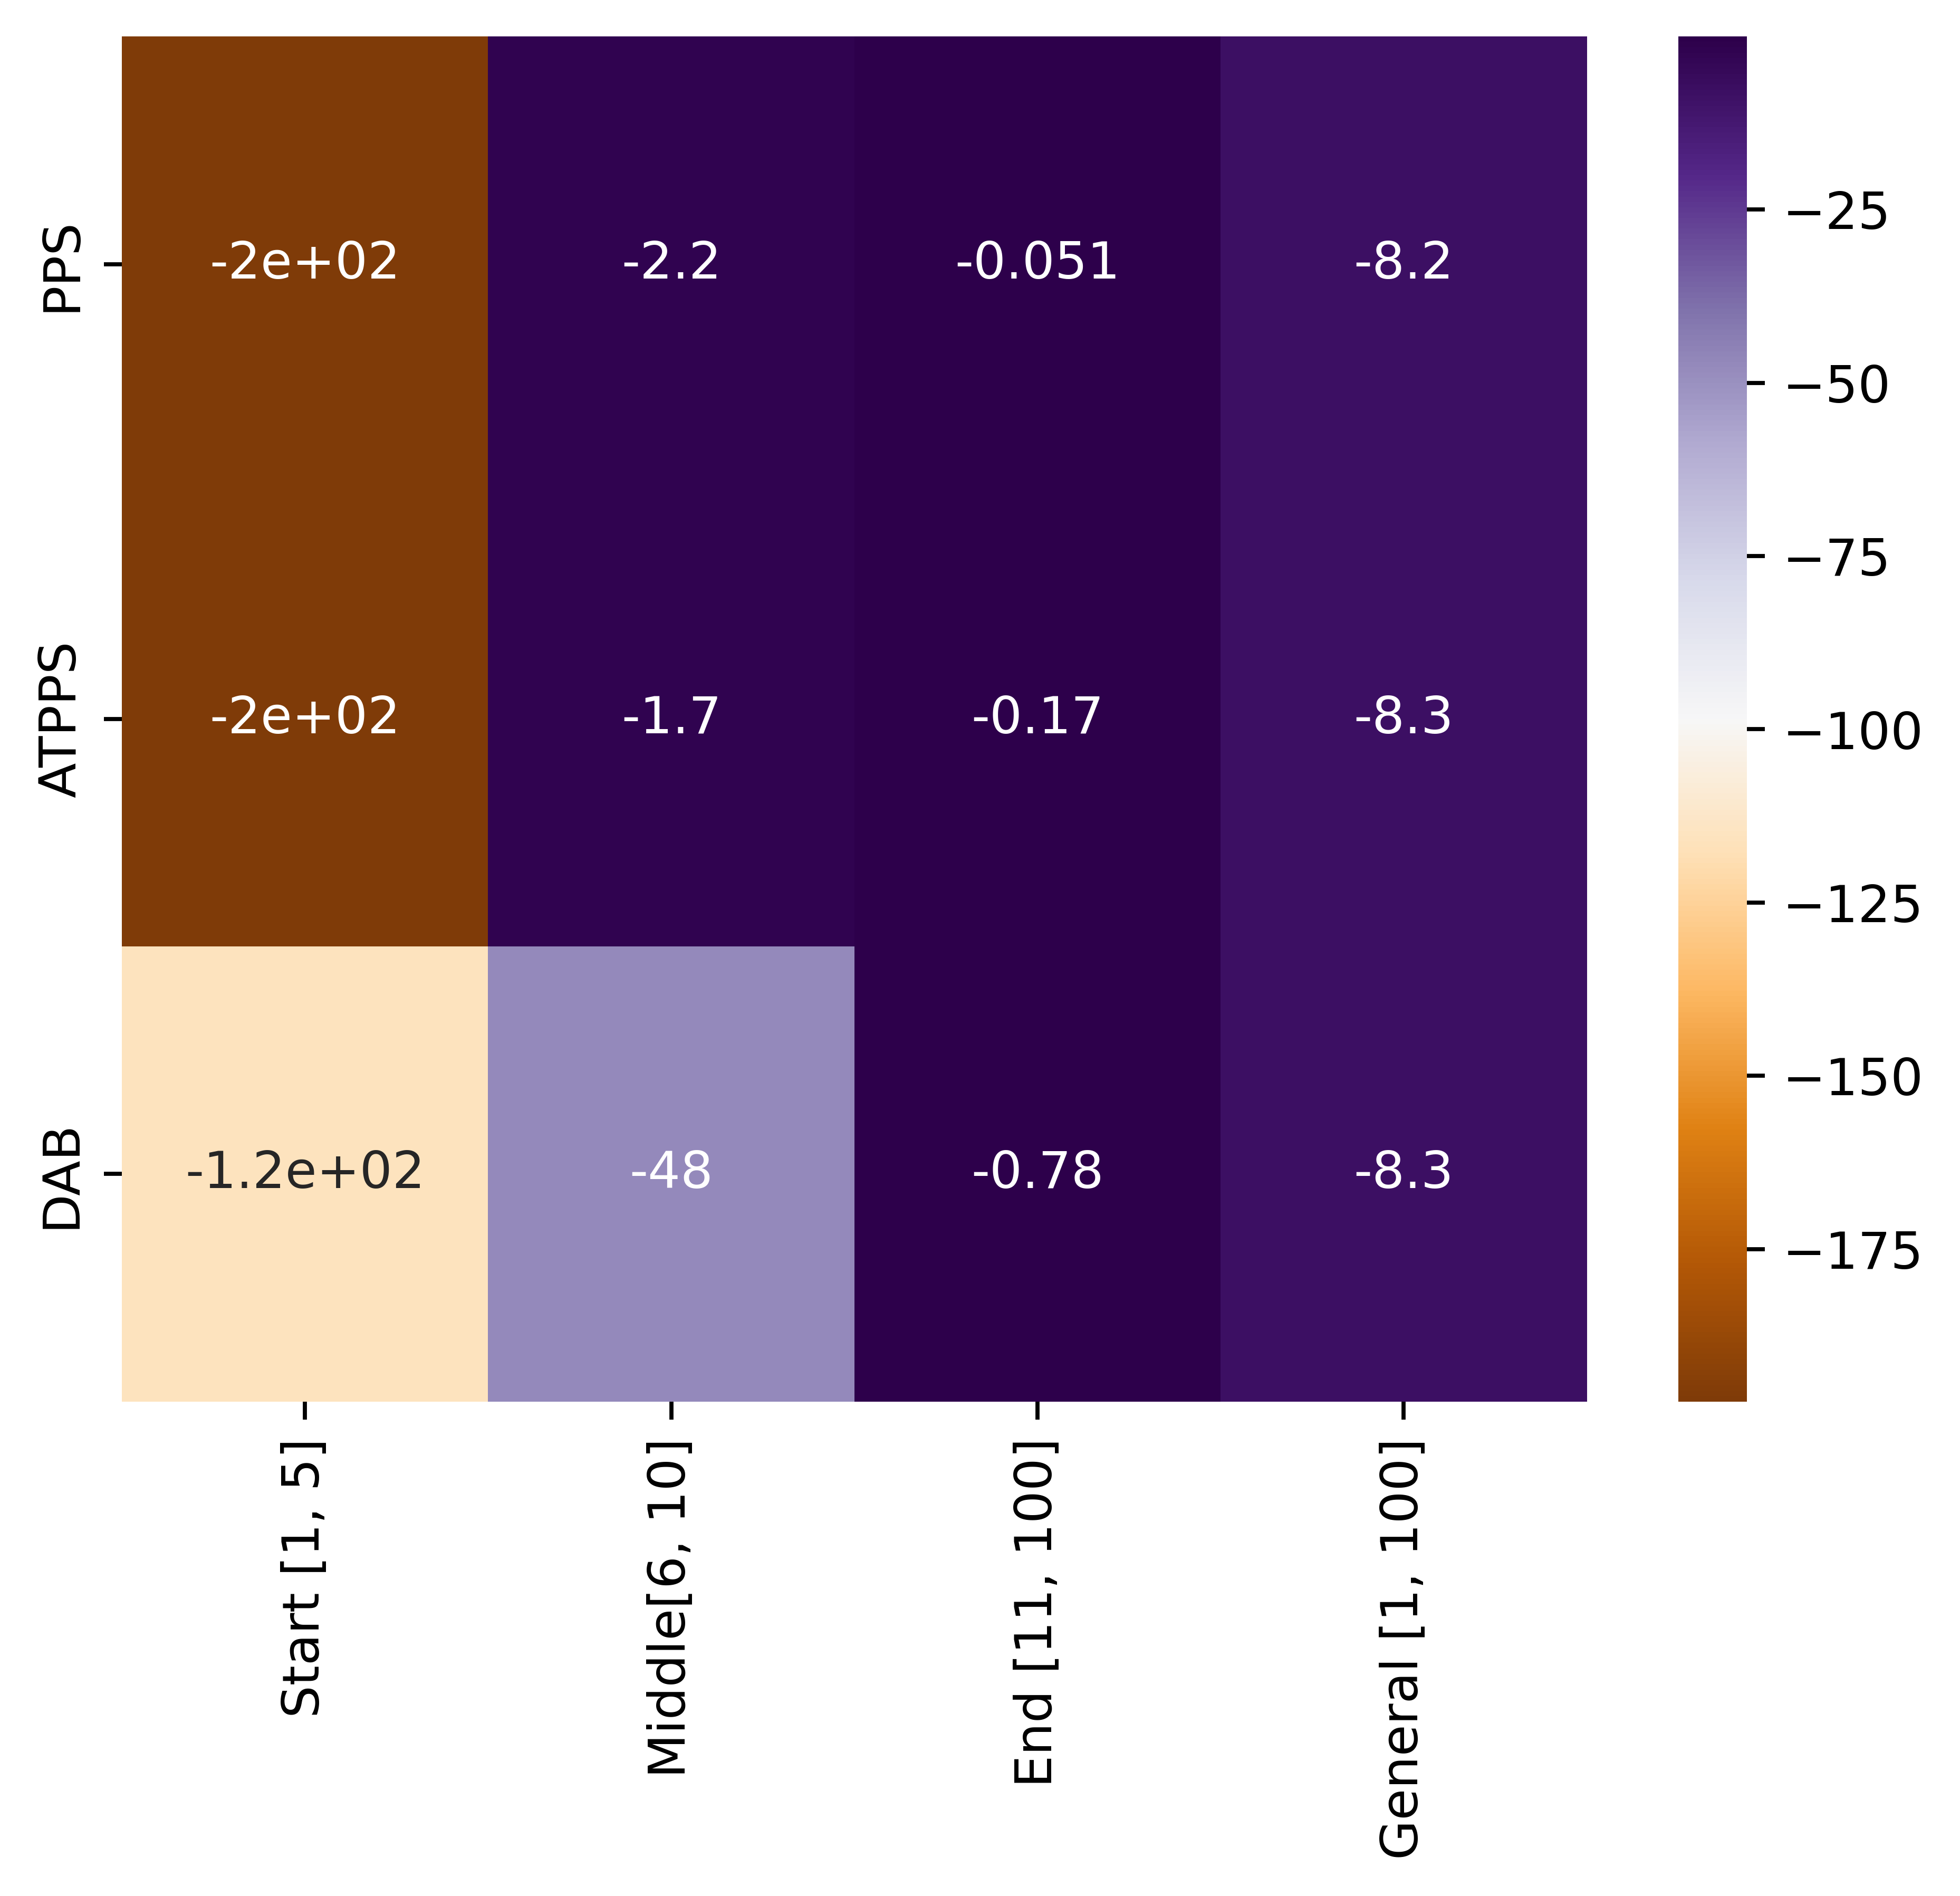
\includegraphics{figures/Simulation_outcomes/RingOfCliques/DAB_vs_PPS_vs_ATPPS_slopesheatmap_100rounds.png}}
%^    \caption{Ring of Cliques: heat map of slopes per region}
%^    \label{fig:ringOfCliquesslopes}
%^\end{figure}

\section{Lollipop Graph}\label{sec:lollipopgraph}
Figure \ref{fig:lollipopgraphMSEperRoundLogLog} shows the three curves of the load balancing algorithms. The ATPPS curve slightly outperforms the PPS curve. The DAB curve lacks to perform as good as the other two load balancing algorithms in reducing the error. The superior performance of PPS compared to DAB in the lollipop graph can be explained by the structure of the graph and the fundamental differences in how these algorithms operate. The clique region consists of high connectivity and enables rapid local balancing for the PPS based algorithms. The path region consists of limited connectivity slows down information propagation and balancing for the PPS based algorithms and favors the deterministic algorithm DAB. The initial discrepancy in the first 10 rounds is due to the potentialy fast decrease of error for the PPS in complete graphs. The DAB load balancing algorithm struggles to perform good in this scenario as observed in section \ref{sec:completeGraph}. The DAB performs rather well in the path graph which in theory is similar to the ring graph without the edge connecting the first and last nodes as described in section \ref{sec:ringgraph}. It prioritizes nodes with the least load, which can lead to inefficient propagation along the complete graph. Load imbalances in the clique region take longer to converge because DAB doesn't exploit the random spreading mechanism of PPS-based algorithms In the initial phase PPS rapidly reduces the MSE, demonstrating strong initial convergence. This quick decrease is due to PPS's proportional load-splitting behavior, which diffuses load across neighbors efficiently in the highly connected clique portion of the lollipop graph. In this region the PPS based algorithms achieve a steep downwards slope with value -130 between rounds 1 to 7, while the DAB reaches nearly half of it with value -67 (figure \ref{fig:lollipopslopes}) In the mid-to-late phase the slope flattens for both of the PPS-based algorithms, indicating slower convergence this is also indicated by the slopes droping to as low as $-0.12 to \sim-0.9$. In this phase, the path section of the lollipop graph dominates the residual imbalances. The adaptive PPS achieves nearly identical behavior to the PPS in the early rounds, as it starts with similar proportional strategies. Adaptive PPS outperforms the PPS slightly in the later rounds due to its ability to dynamically adjust its balancing strategy based on the current state of load imbalances. This allows it to better address residual imbalances in the path section of the lollipop graph as showcased in section \ref{sec:ringgraph}.

The DAB model fit follows the equation: $MSE_r=-5.89\times10^{-5}r^{3}+0.03r^{2}-5.68r+459.42$, which is a 4-th degree polynomial equation. The PPS and ATPPS are a bit more complex and expressed by a polynomial equation of degree 5. The PPS model fit follows the equation: $MSE_r=8.44\times 10^{-07}r^{4}-2.52\times 10^{-4}r^{3}-0.03r^{2}-1.64r+56.68$ and the ATPPS model fit follows the equation: $MSE_r=8.69 \times 10^{-07}r^{4}-2.56 \times 10^{-4}r^{3}+0.03r^{2}-1.62r+54.48$.

%\begin{figure}[h]
%    \centering
%    \scalebox{0.5}{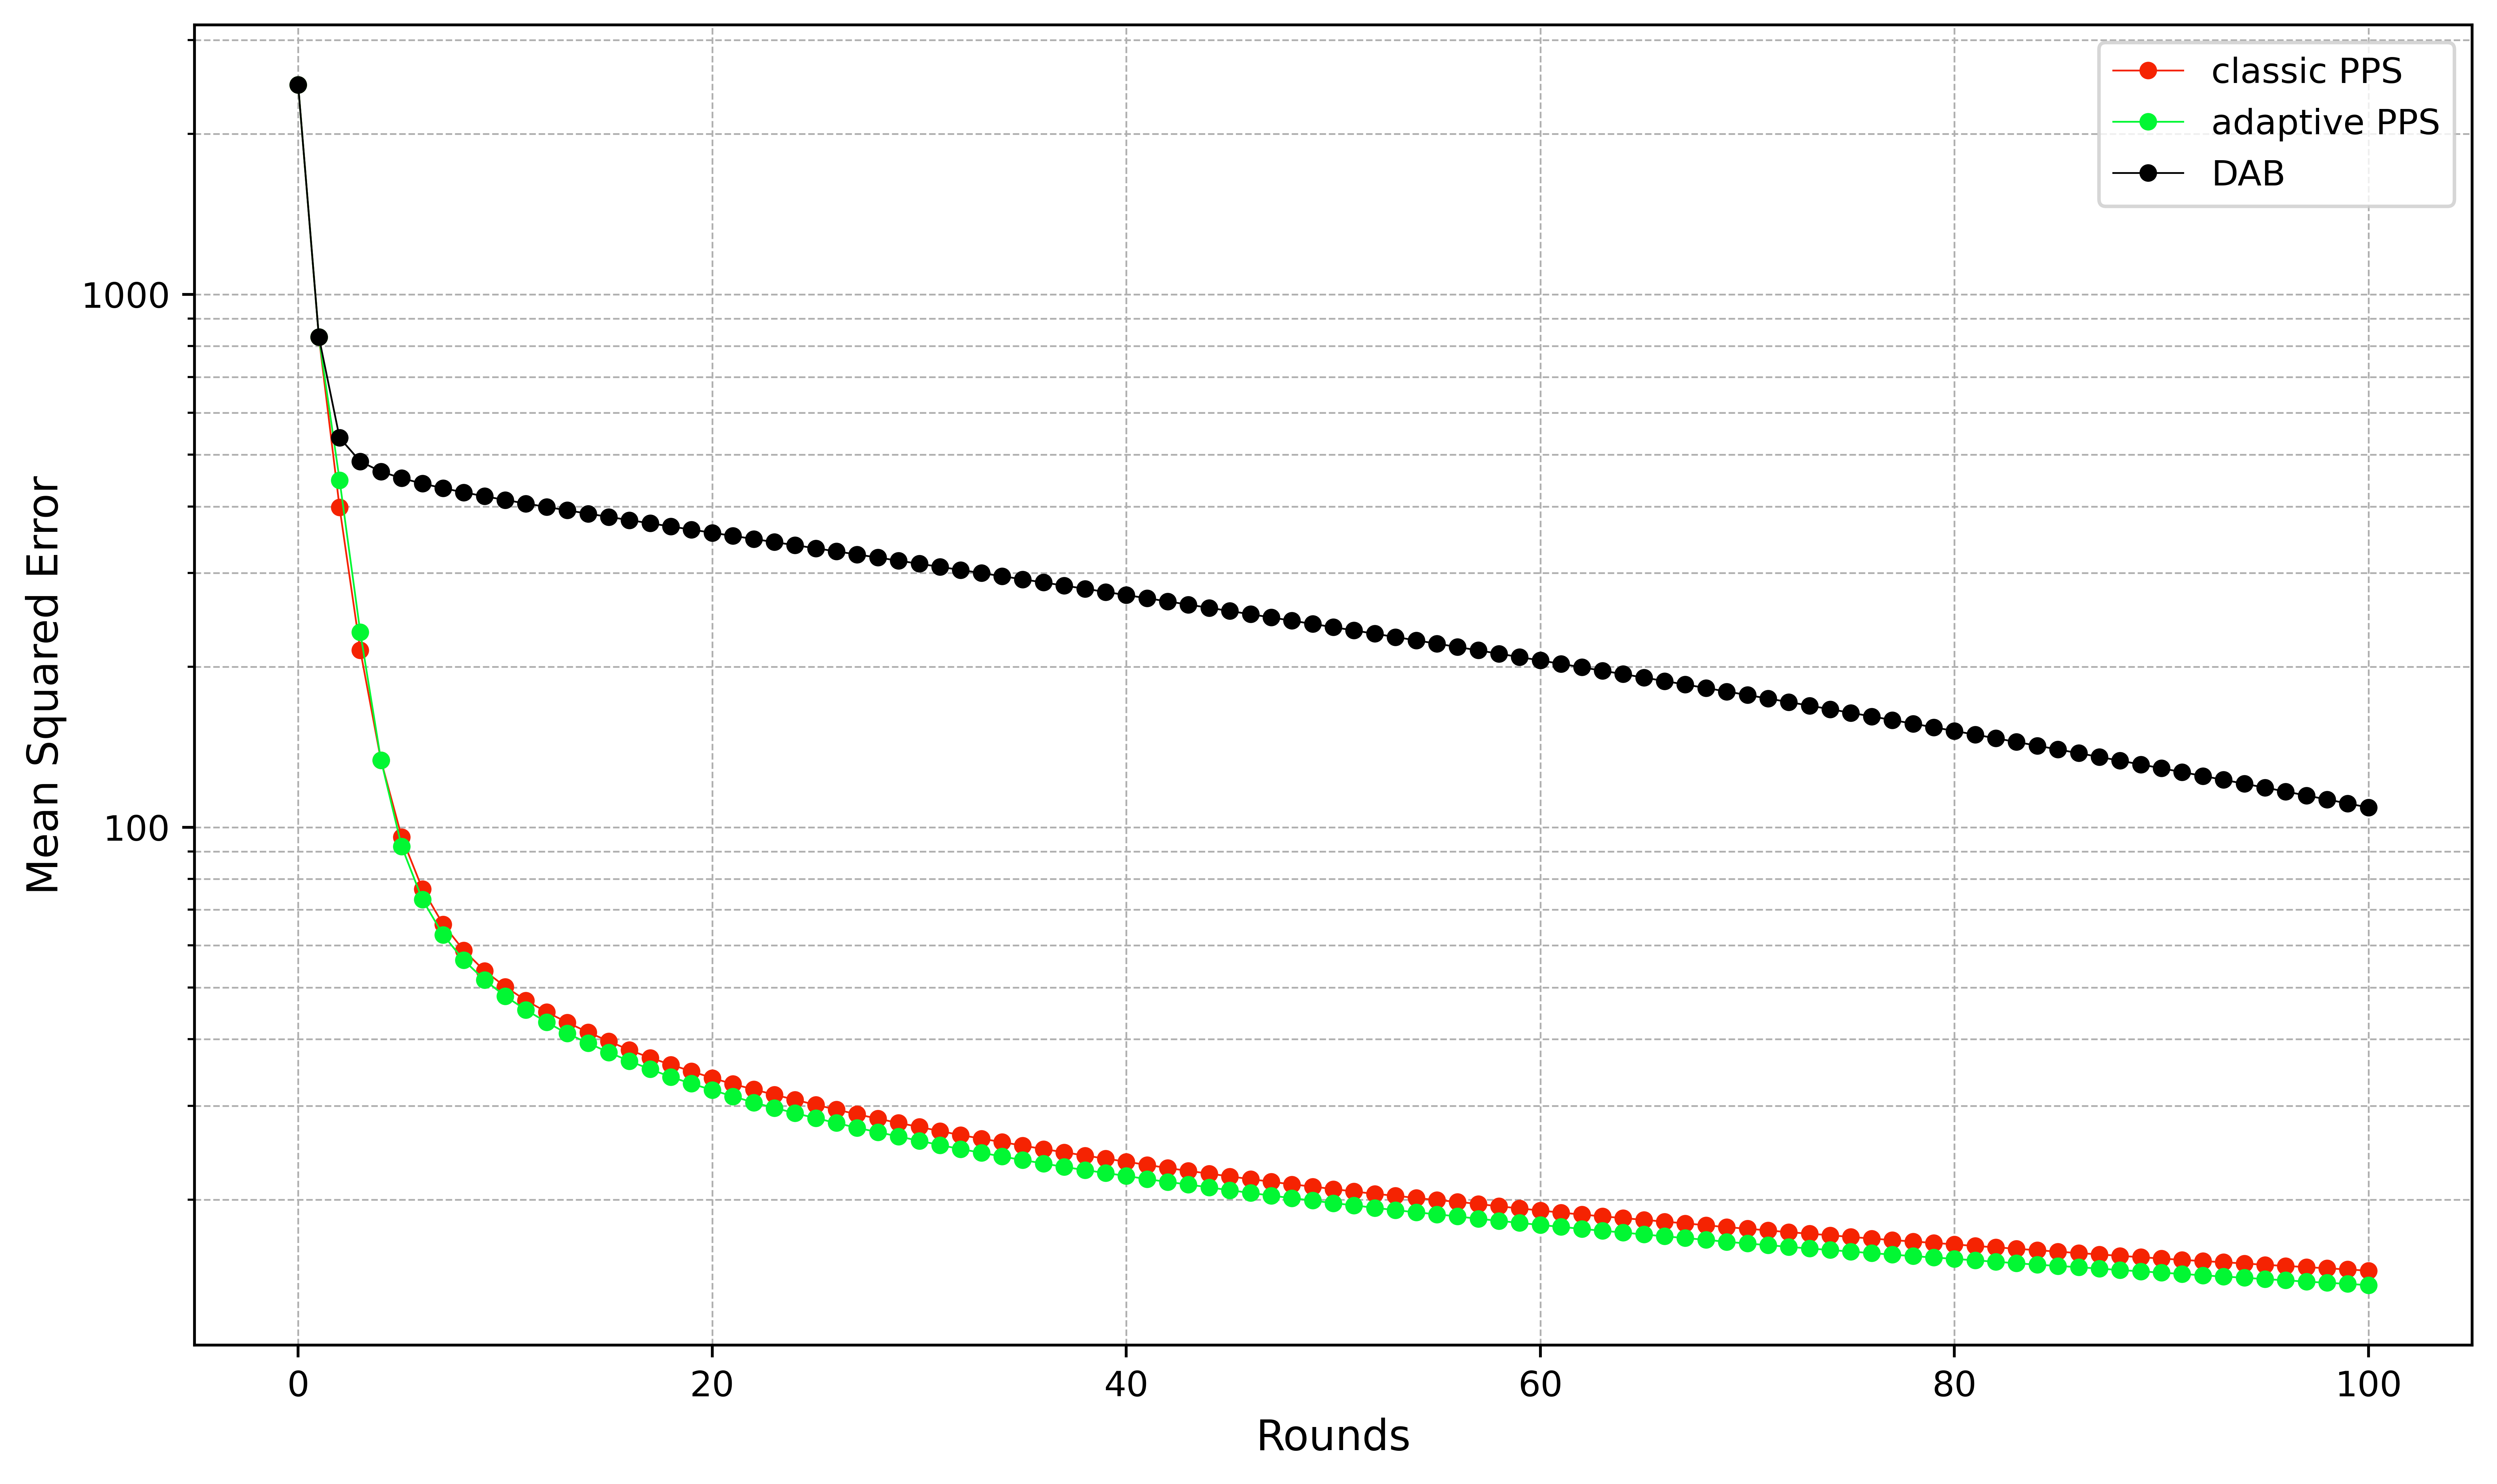
\includegraphics{figures/Simulation_outcomes/LollipopGraph/DAB_vs_PPS_LG_r100_n1024_averaged_log.png}}
%    \caption{Lollipop Graph: mean squared error per rounds (log-linear)}
%    \label{fig:lollipopgraphMSEperRoundLogLog}
%\end{figure}
%
%\begin{figure}[H]
%    \centering
%    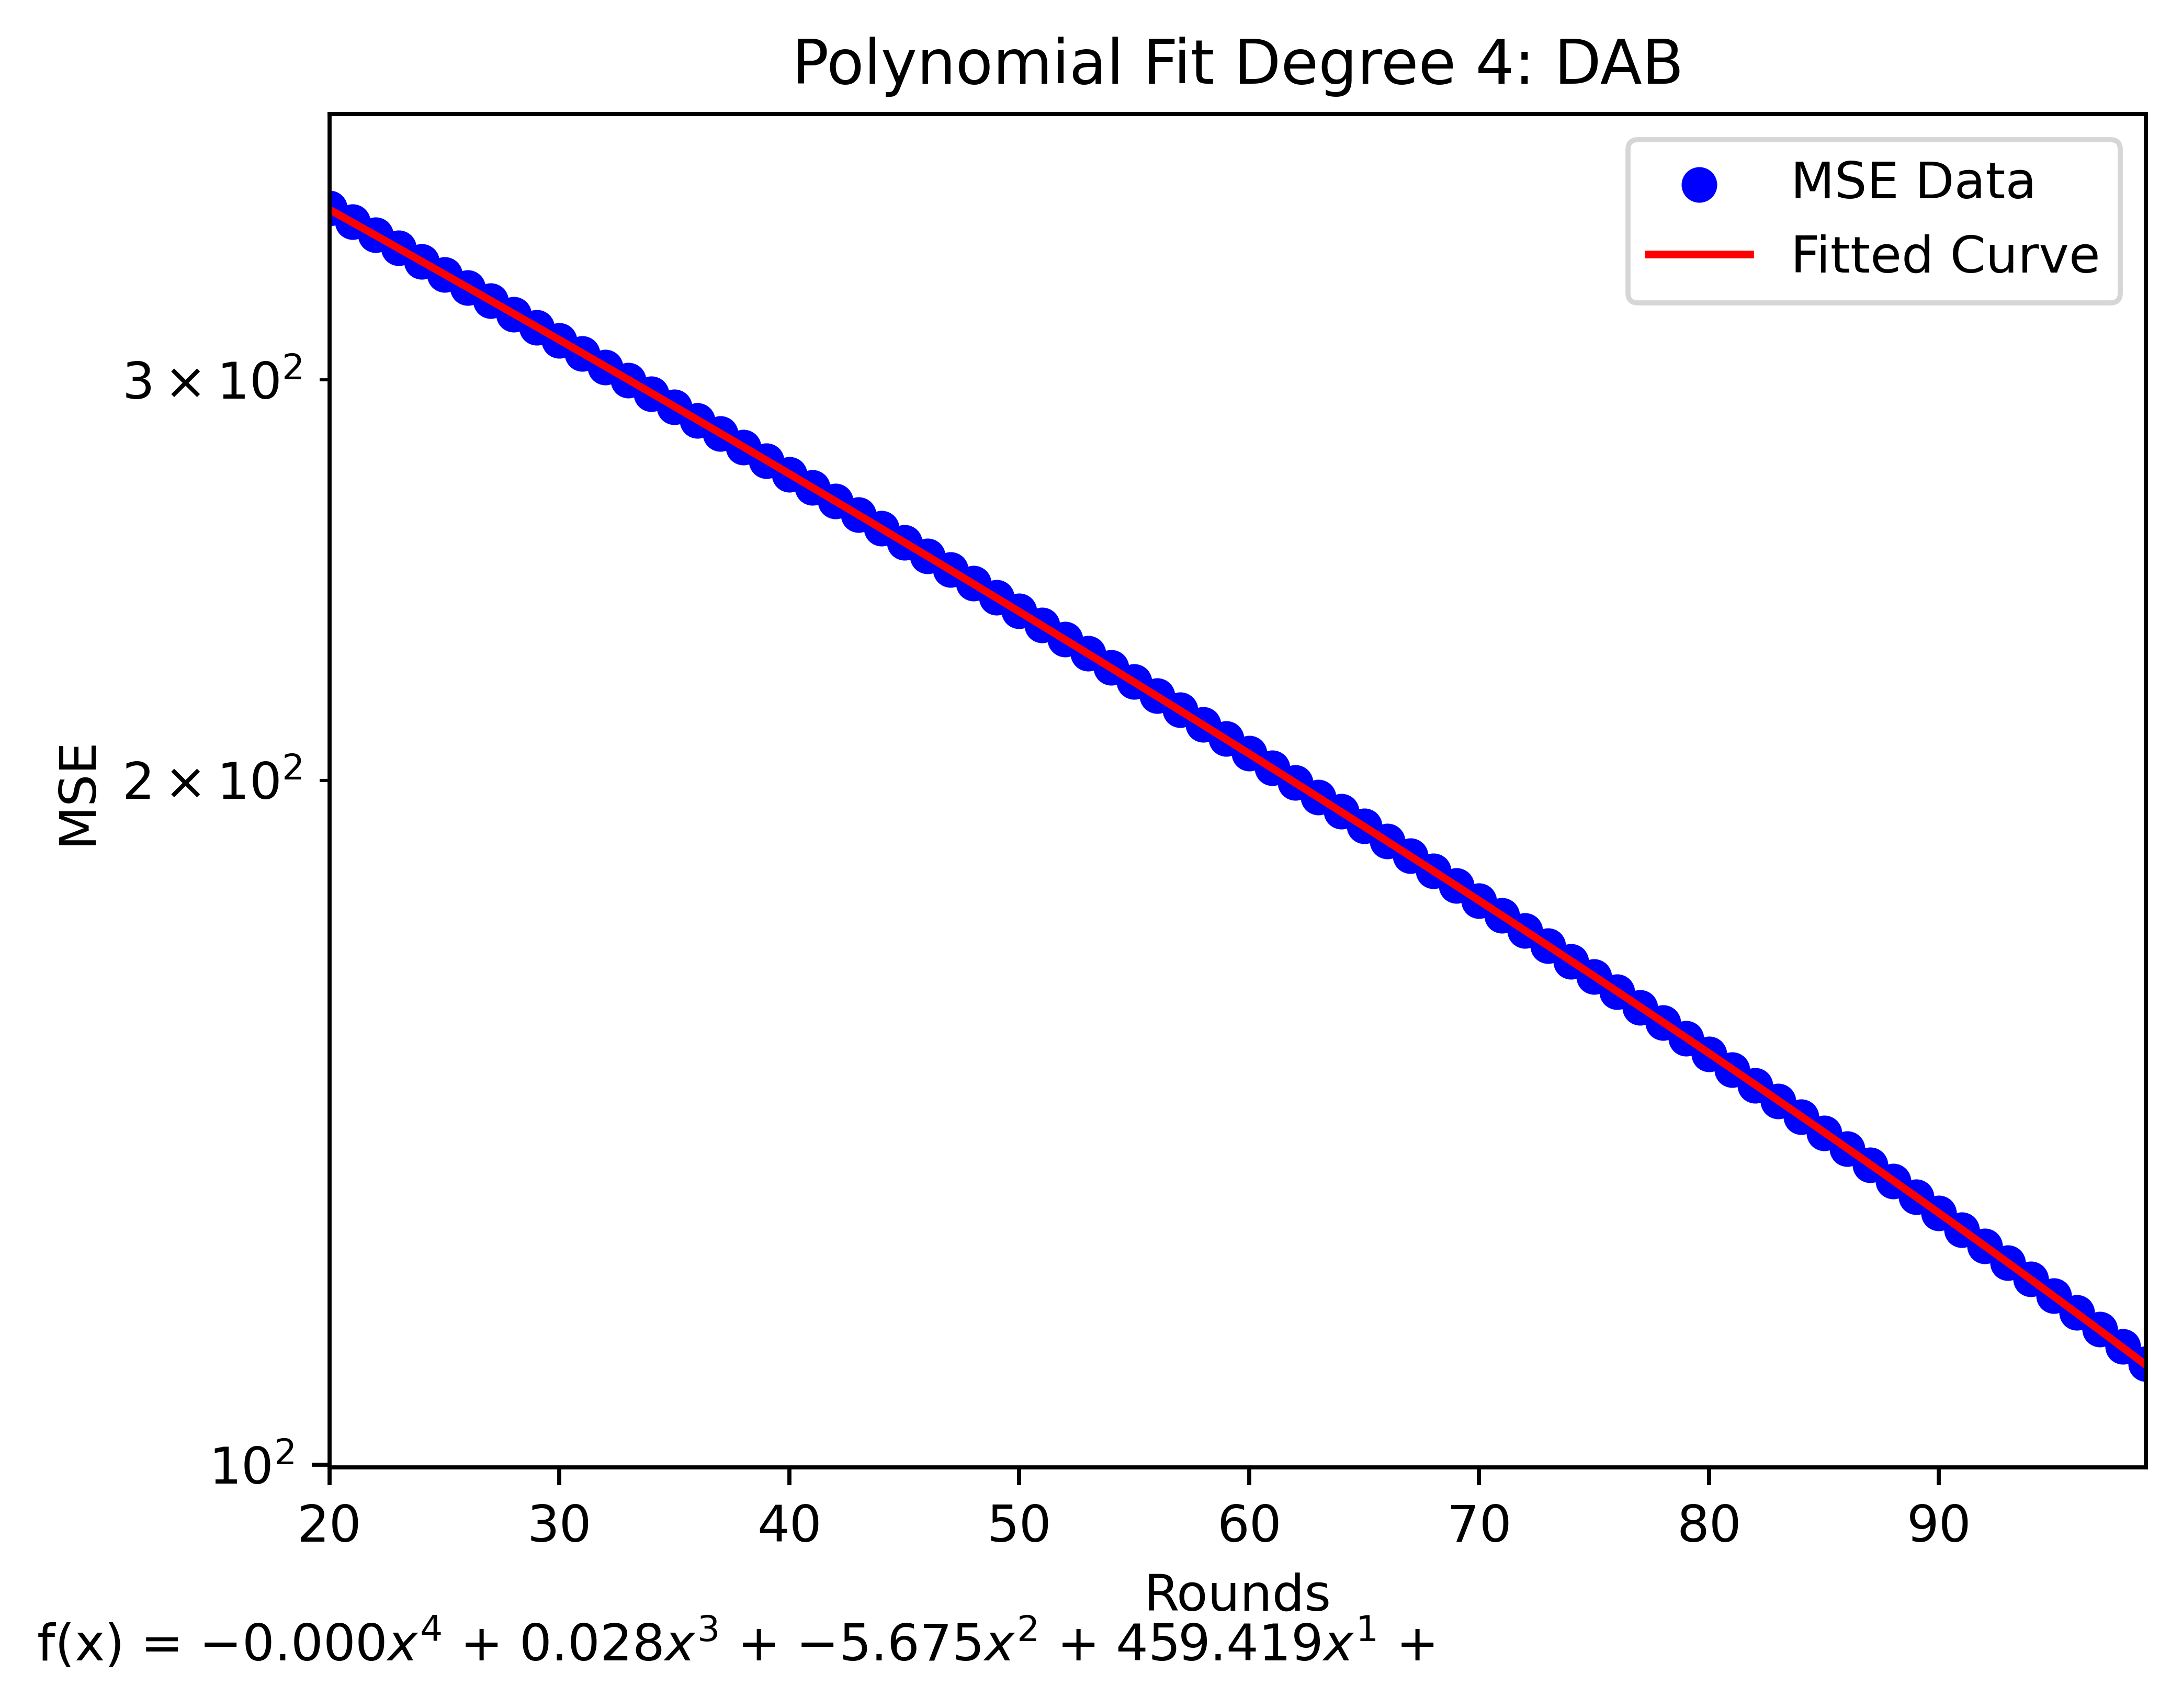
\includegraphics[width=\linewidth]{figures/Simulation_outcomes/LollipopGraph/DAB/DAB_modelfitting_rounds_99_model_2.png}
%    \caption{Polynomial Regression Fit: DAB}
%    \label{fig:dablollipopgraphModelFit}
%\end{figure}
%
%\begin{figure}[H]
%    \centering
%    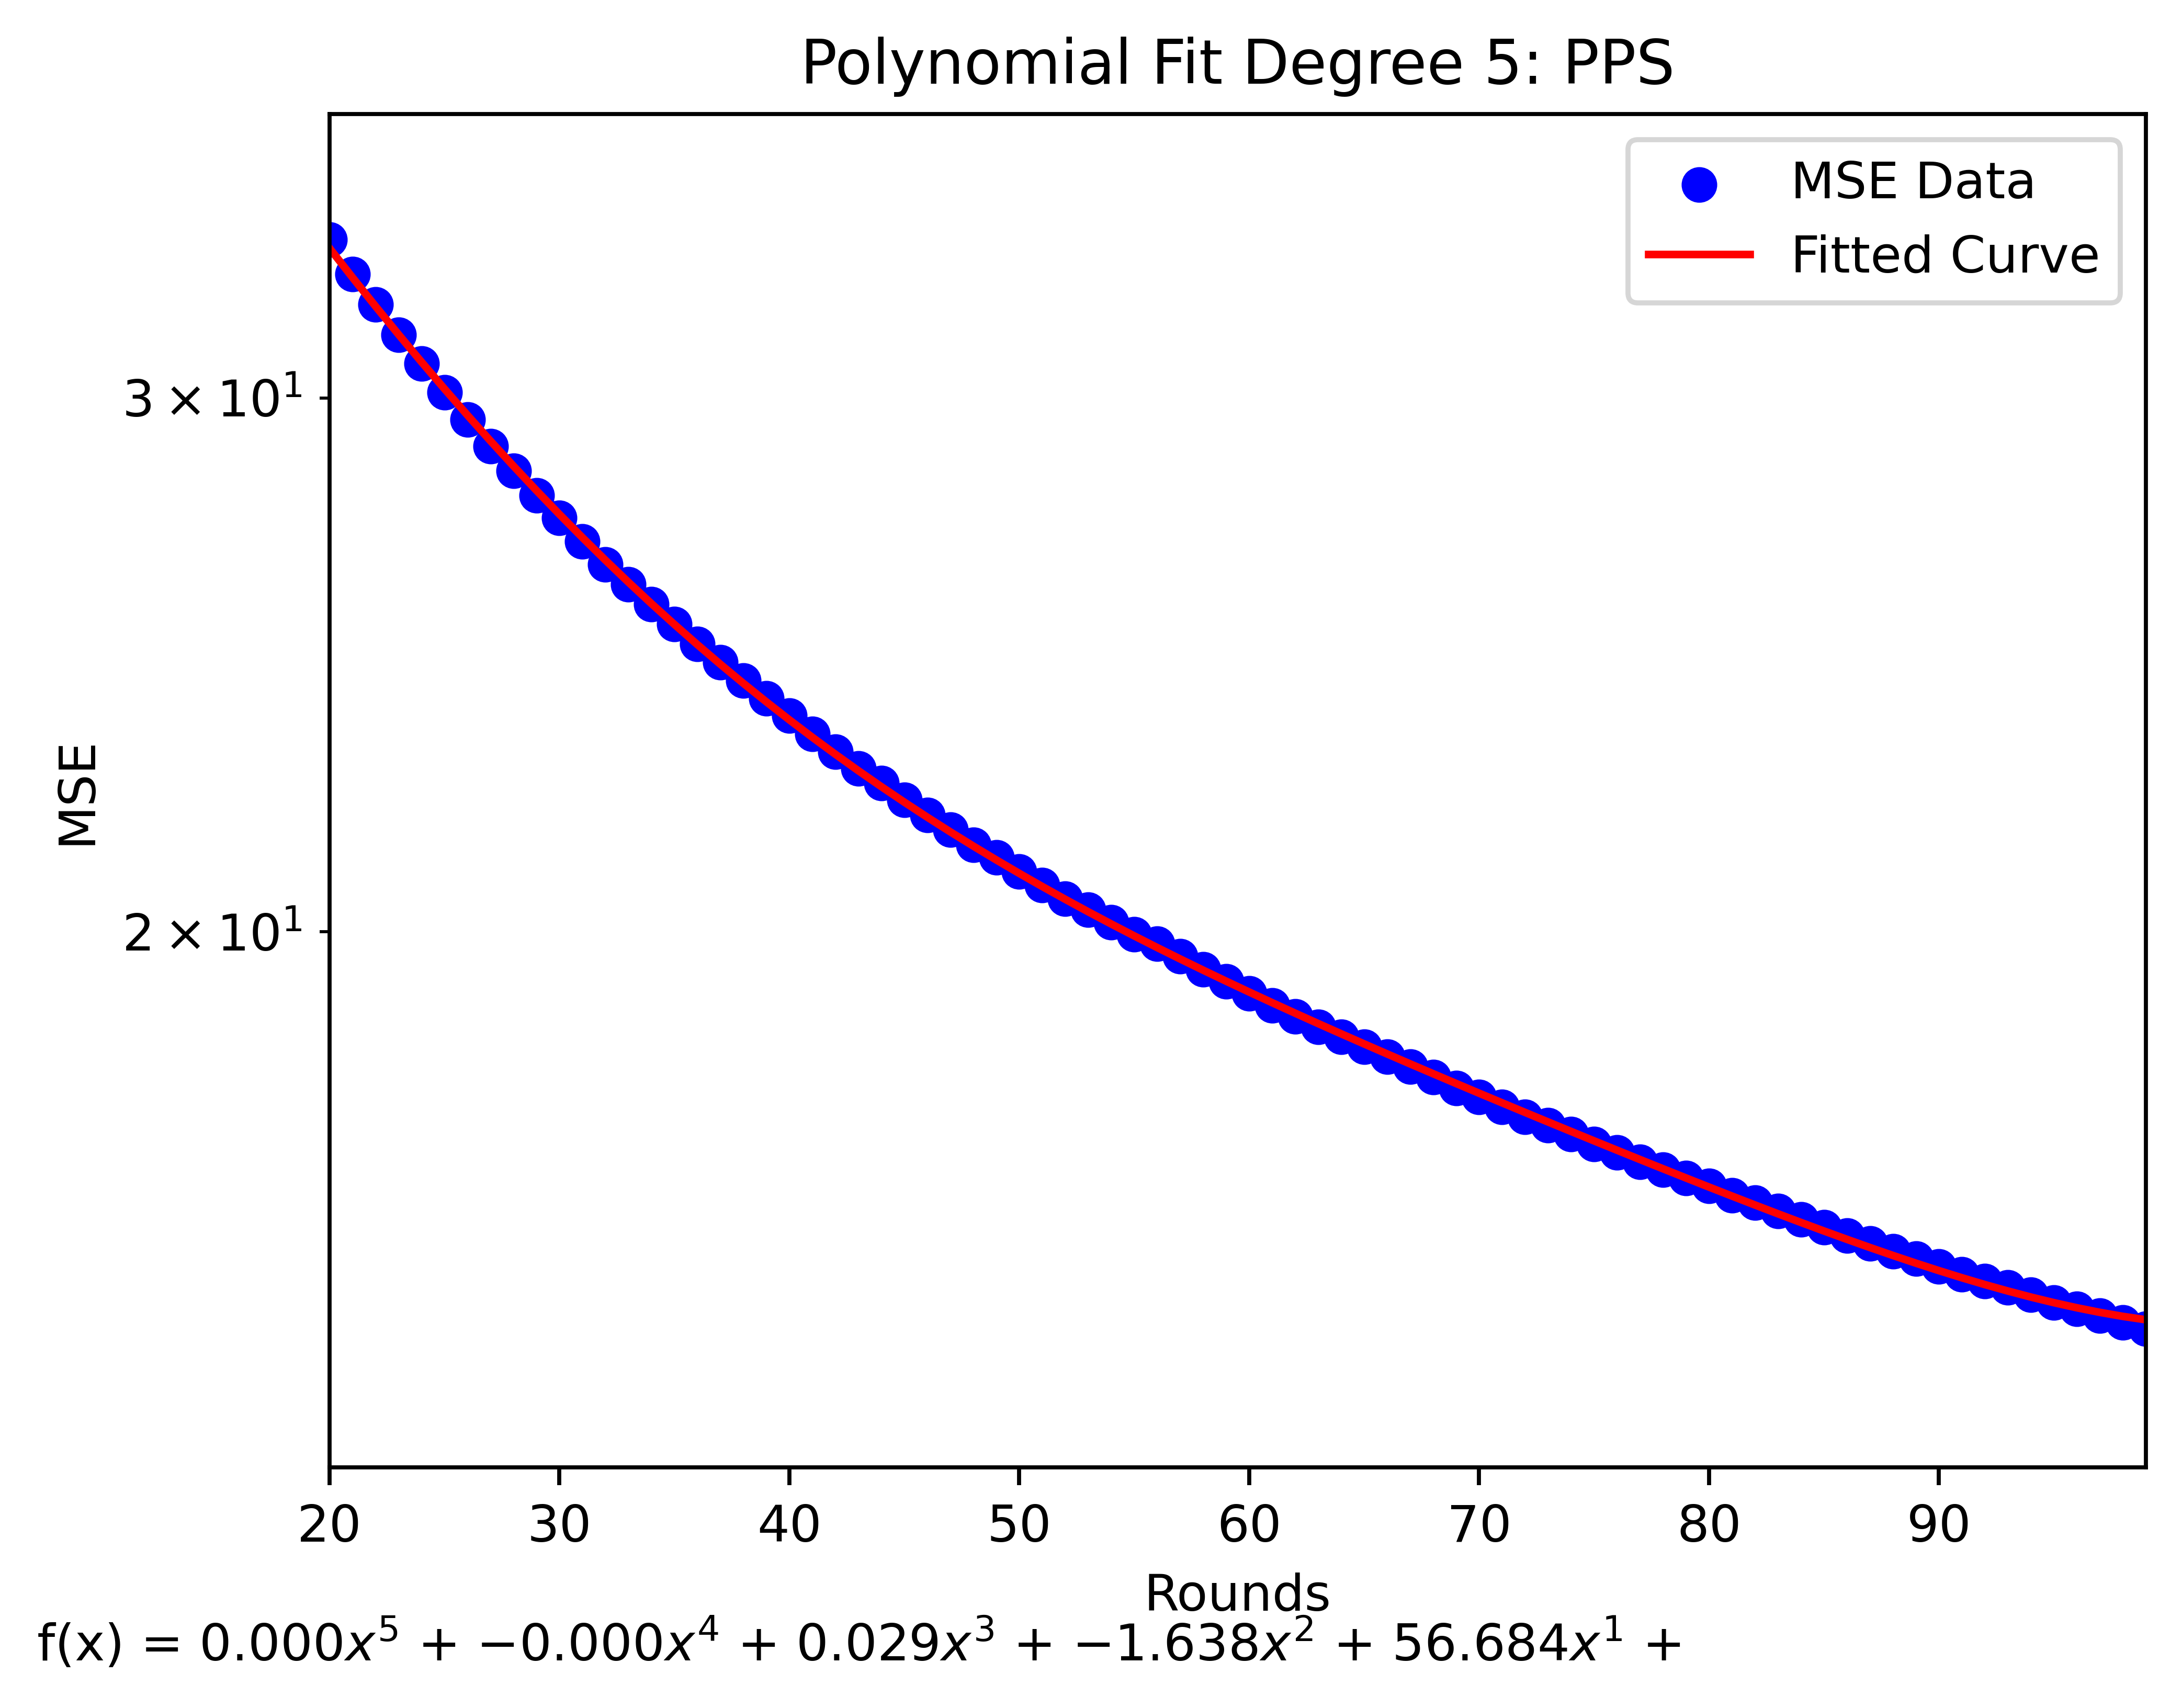
\includegraphics[width=\linewidth]{figures/Simulation_outcomes/LollipopGraph/PPS/PPS_modelfitting_rounds_99_model_2.png}
%    \caption{Polynomial Regression Fit: DAB}
%    \label{fig:ppslollipopgraphModelFit}
%\end{figure}
%
%\begin{figure}[H]
%    \centering
%    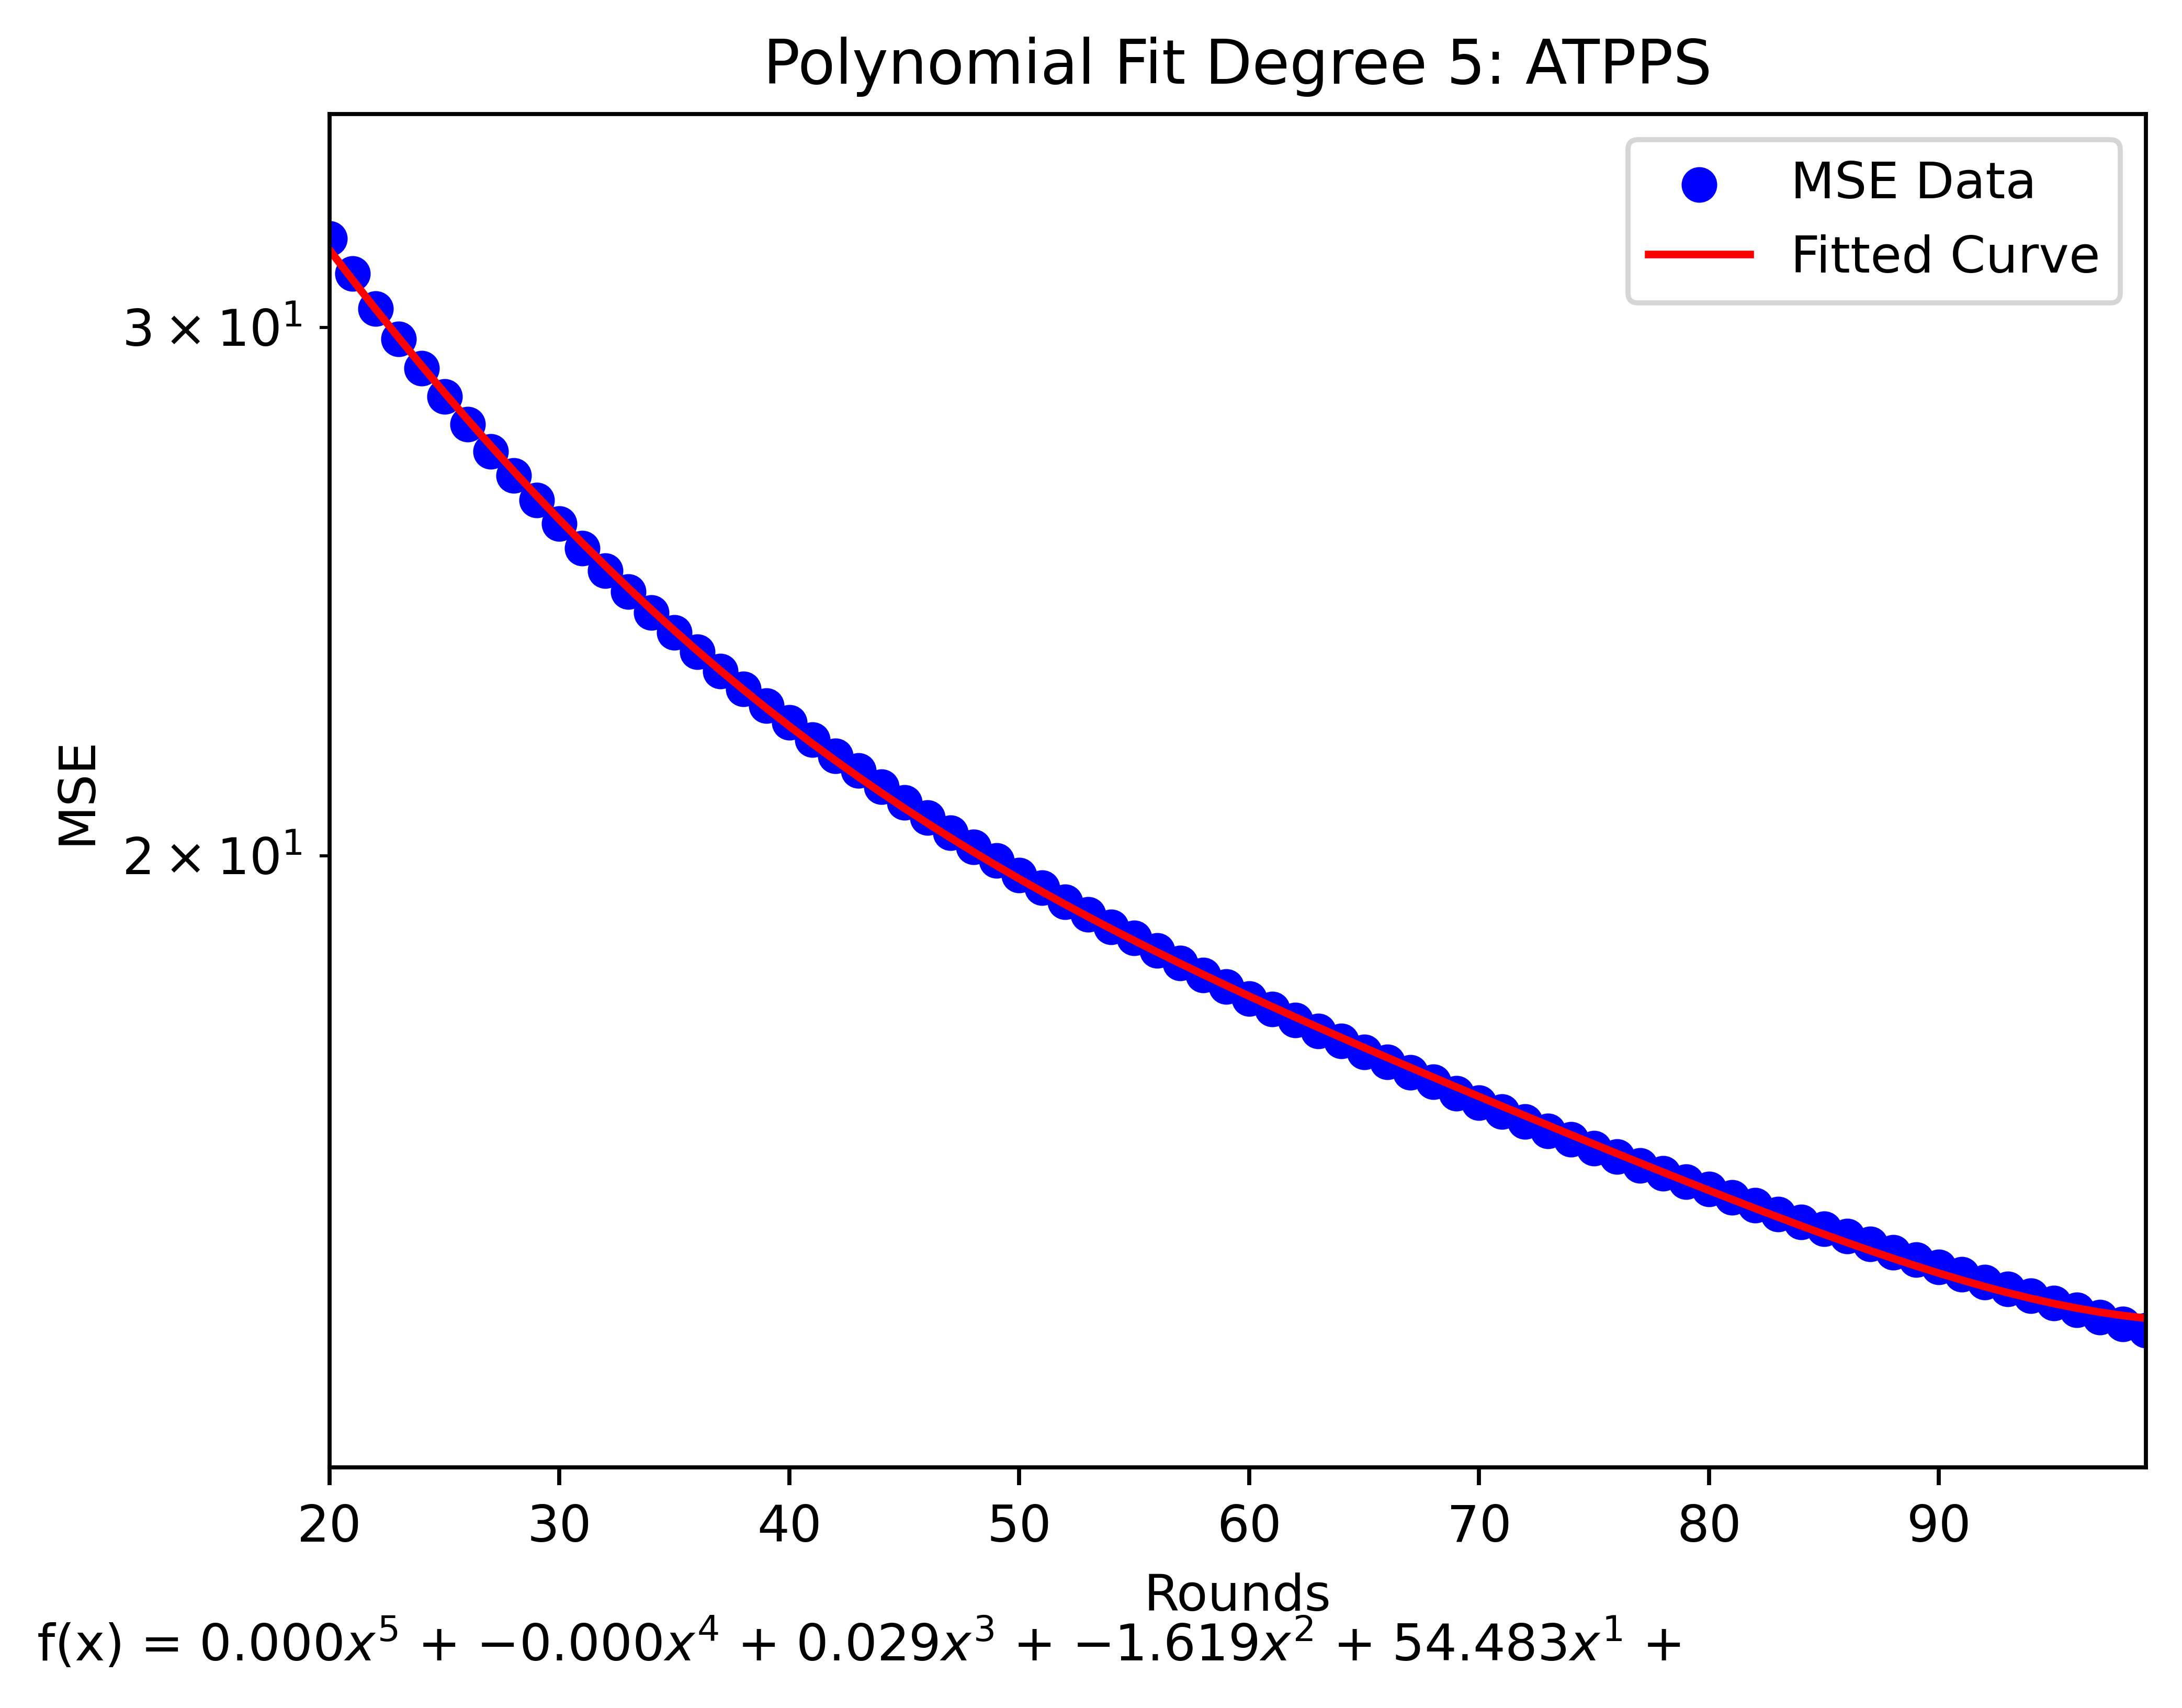
\includegraphics[width=\linewidth]{figures/Simulation_outcomes/LollipopGraph/ATPPS/ATPPS_modelfitting_rounds_99_model_2.png}
%    \caption{Polynomial Regression Fit: DAB}
%    \label{fig:atppslollipopgraphModelFit}
%\end{figure}
%
%\begin{figure}
%    \centering
%    \scalebox{0.8}{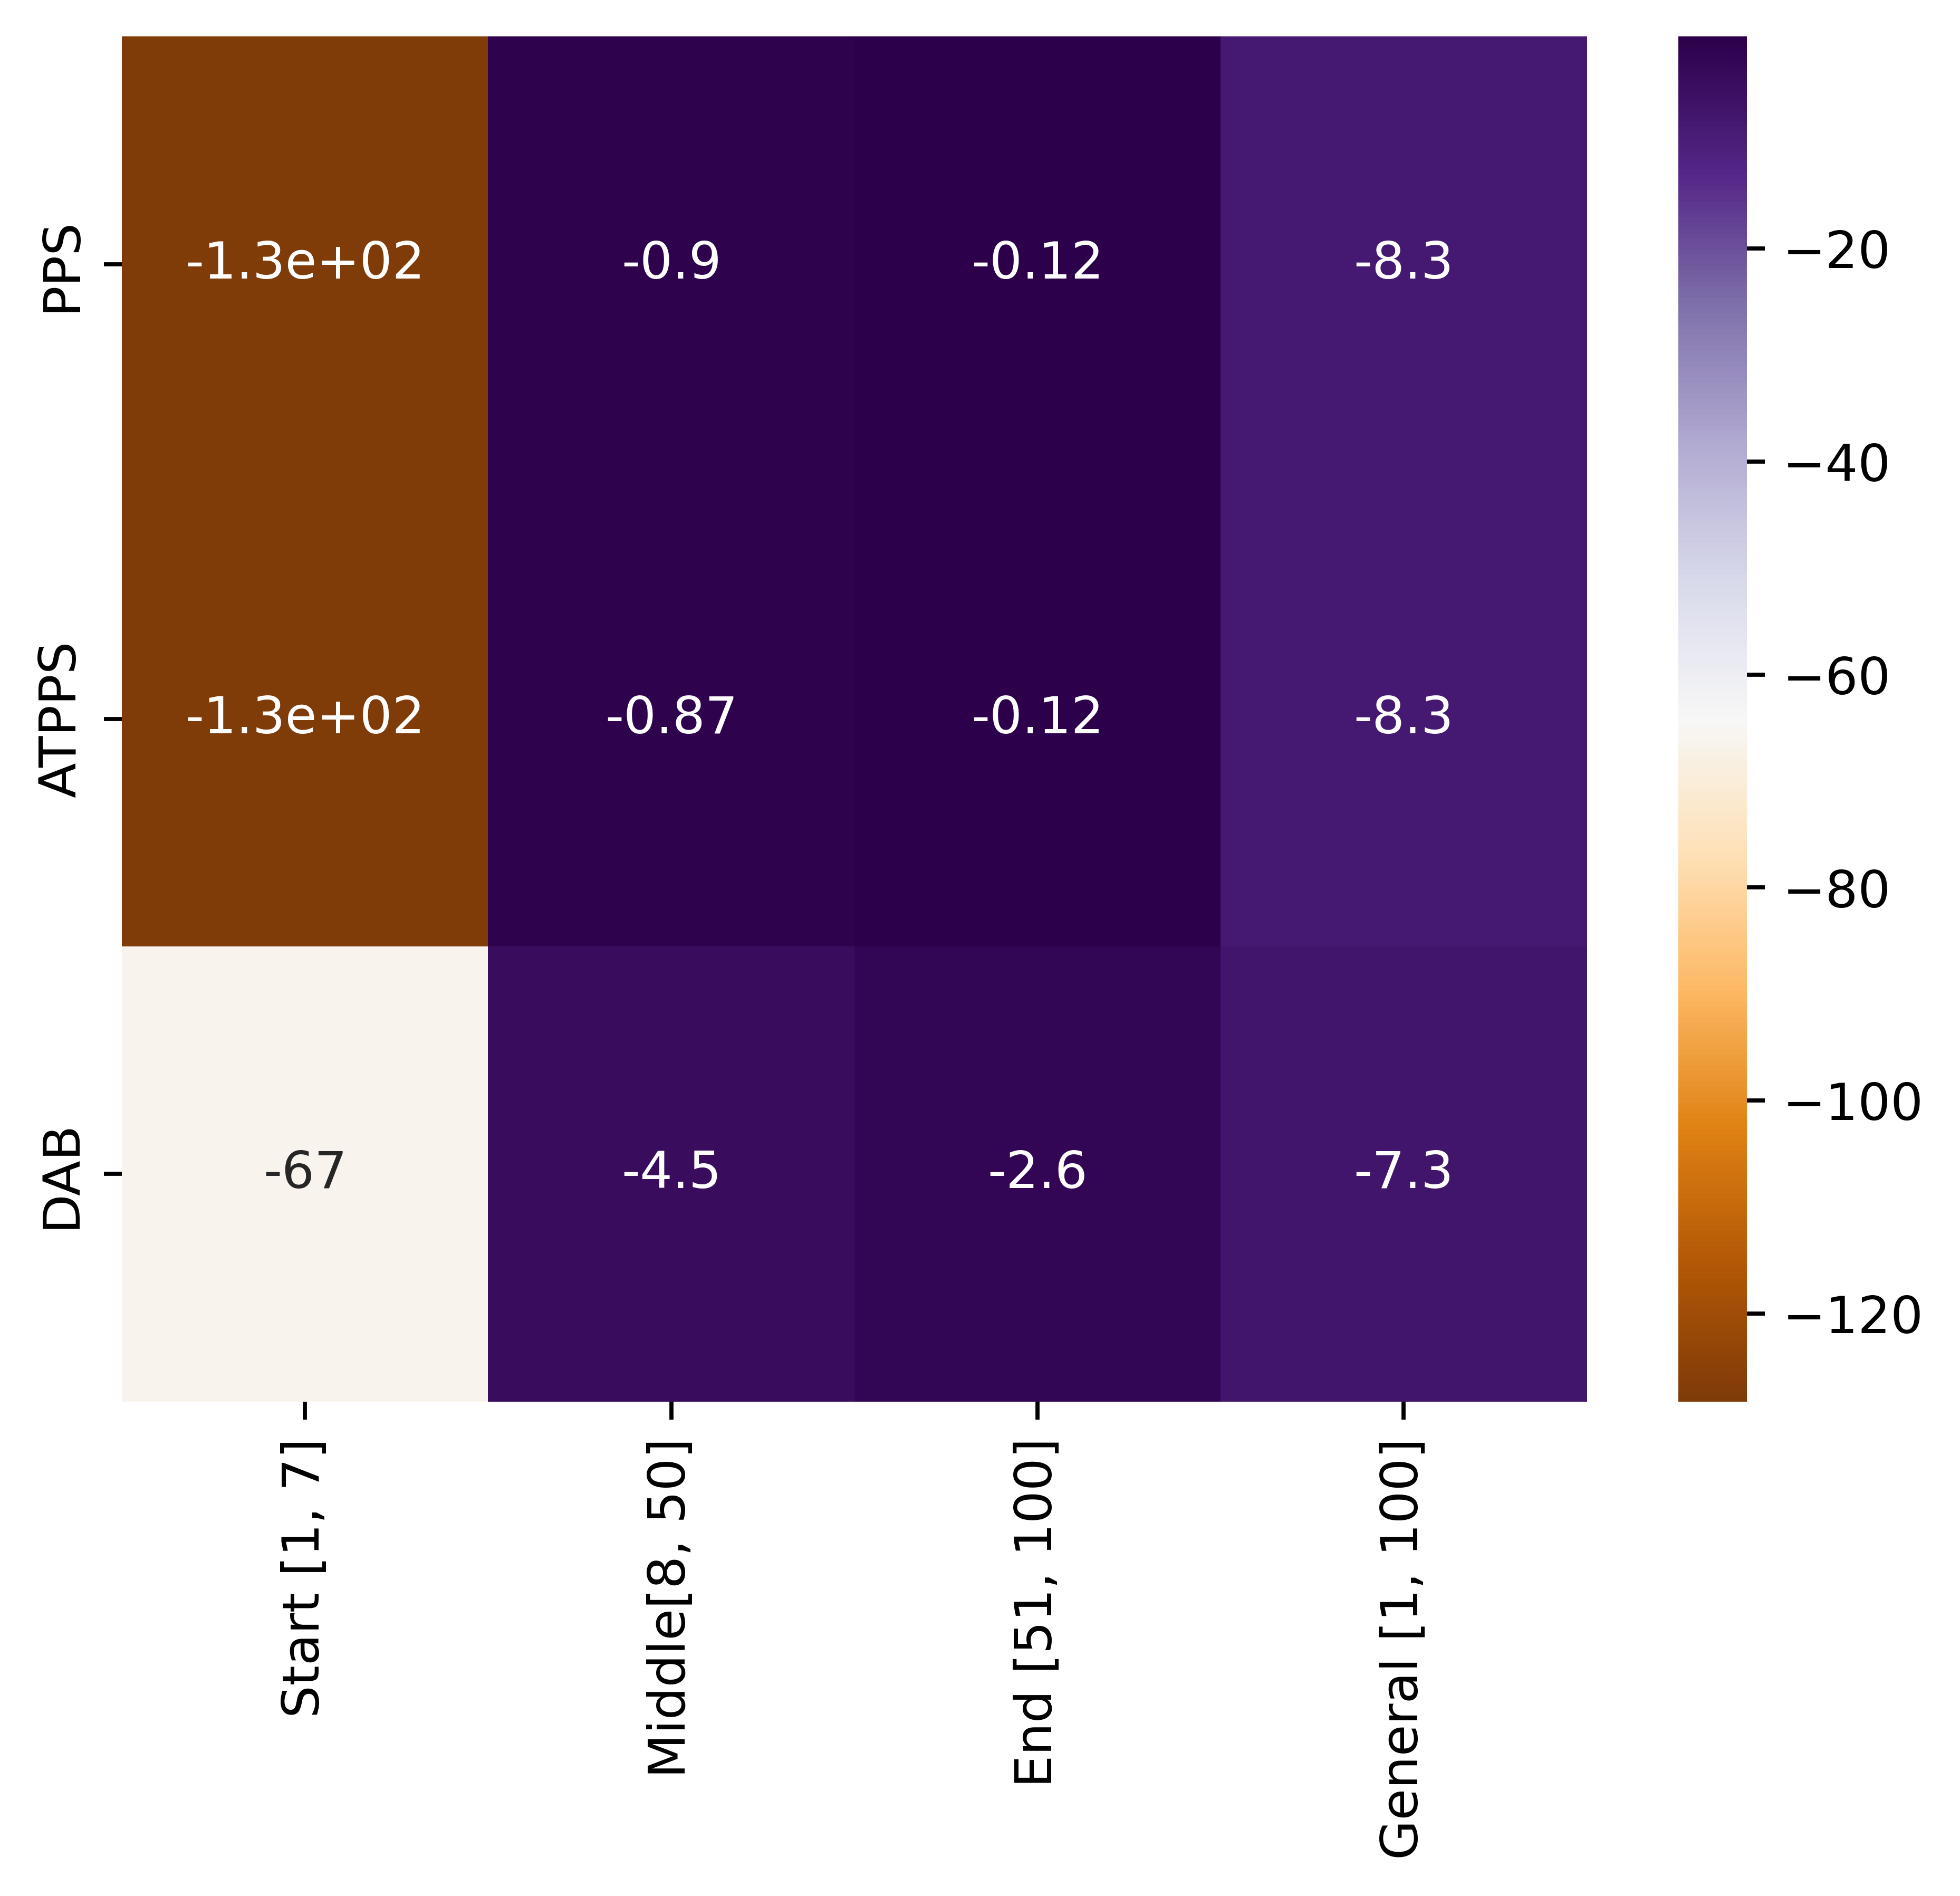
\includegraphics{figures/Simulation_outcomes/LollipopGraph/DAB_vs_PPS_vs_ATPPS_slopesheatmap_100rounds.png}}
%    \caption{Lollipop Graph: heat map of slopes per region}
%    \label{fig:lollipopslopes}
%\end{figure}